\documentclass[hyperref=colorlinks]{beamer}
\mode<presentation>
\usetheme{iclpt}
\setbeamertemplate{navigation symbols}{}
\setbeamertemplate{headline}{
\begin{beamercolorbox}[leftskip=.2cm,rightskip=.2cm,topskip=.2cm,ht=1.1cm,dp=0.1cm,wd=\textwidth]{institute in head/foot}
  
\includegraphics[height=1cm]{icl.pdf}
  \hfill
  
\includegraphics[height=1cm]{../Pics/CMS-Color.pdf}
\end{beamercolorbox}
}
\setbeamertemplate{footline}{
\begin{beamercolorbox}[ht=.55cm,dp=0.4cm,wd=\textwidth,leftskip=.3cm]{author in head/foot}%
  \begin{minipage}[c]{5cm}%
    \usebeamerfont{author in head/foot}
    \insertshortauthor 
    \insertshorttitle
    \end{minipage}\hfill%
  \insertframenumber{} / \pageref{lastframe}
  \hfill
  \begin{minipage}{6cm}
    \hfill
  \end{minipage}
\end{beamercolorbox}%
}

\usepackage{color}
\usepackage{tabularx,colortbl}
\usepackage{graphicx}
\usepackage{pdfpages}
\usepackage{feynmp}
\DeclareGraphicsRule{*}{mps}{*}{}

\title{\vspace{-0.2cm} VBF Higgs to Invisible - Update}
\subtitle{AN-14-243\vspace{-0.7cm}}
\author[P. Dunne]{\underline{P. Dunne} on behalf of the VBF H$\rightarrow$invisible analysis group} % A.M. Magnan and A. Nikitenko Joao Pela with \\ R. Aggleton, J. Brooke: Bristol \\ C.Asawangtrakuldee, Q.Li: Peking \\ P. Srimanobhas: Chulalongkorn \\ S. Kumar, K. Mazumdar: Mumbai}
\titlegraphic{
  \vspace{-0.7cm}
  %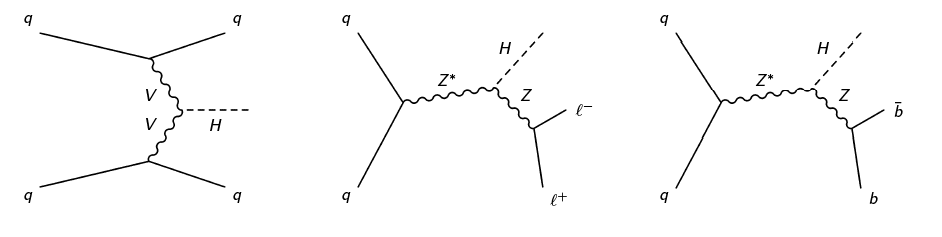
\includegraphics[width=\textwidth]{TalkPics/invcomb021213/feyndiags}
%% \begin{fmfgraph*}(100,70)
%%         \fmfleft{i1,i2}
%%         \fmfright{o1,o2,o3}
%%         \fmf{fermion}{i1,v1,o1}
%%         \fmf{fermion}{i2,v2,o3}
%%         \fmf{phantom,tension=4/5}{v1,v2}
%%         \fmffreeze
%%         \fmf{photon,label=$W,,Z$}{v1,v3}
%%         \fmf{photon,label=$W,,Z$}{v2,v3}
%%         \fmf{dashes}{v3,o2}
%%         \fmflabel{$q$}{i1}
%%         \fmflabel{$q$}{i2}
%%         \fmflabel{$q$}{o1}
%%         \fmflabel{$q$}{o3}
%%         \fmflabel{$H$}{o2}
%%       \end{fmfgraph*}
}
\date{}
\begin{document}
\begin{fmffile}{higgsexoupdatefeyndiags}

%TITLE PAGE
\section{Title}
\begin{frame}
  \titlepage
  
\end{frame}

%THEORY MOTIVATION
\begin{frame}
    \frametitle{Why Higgs to Invisible?}
    \vspace{-.2cm}
    \begin{columns}
      \column{.5\textwidth}
      \begin{block}{\scriptsize Experimental motivation}
        \scriptsize
        \begin{itemize}
        \item Current measurements of the 125 GeV Higgs boson are compatible with Standard Model (SM) expectations
        \item[-] large uncertainties can still accommodate significant beyond the SM (BSM) properties
        \item Additional Higgs bosons with exotic decays are not excluded
        \end{itemize}
      \end{block}
      \column{.45\textwidth}
      \hfill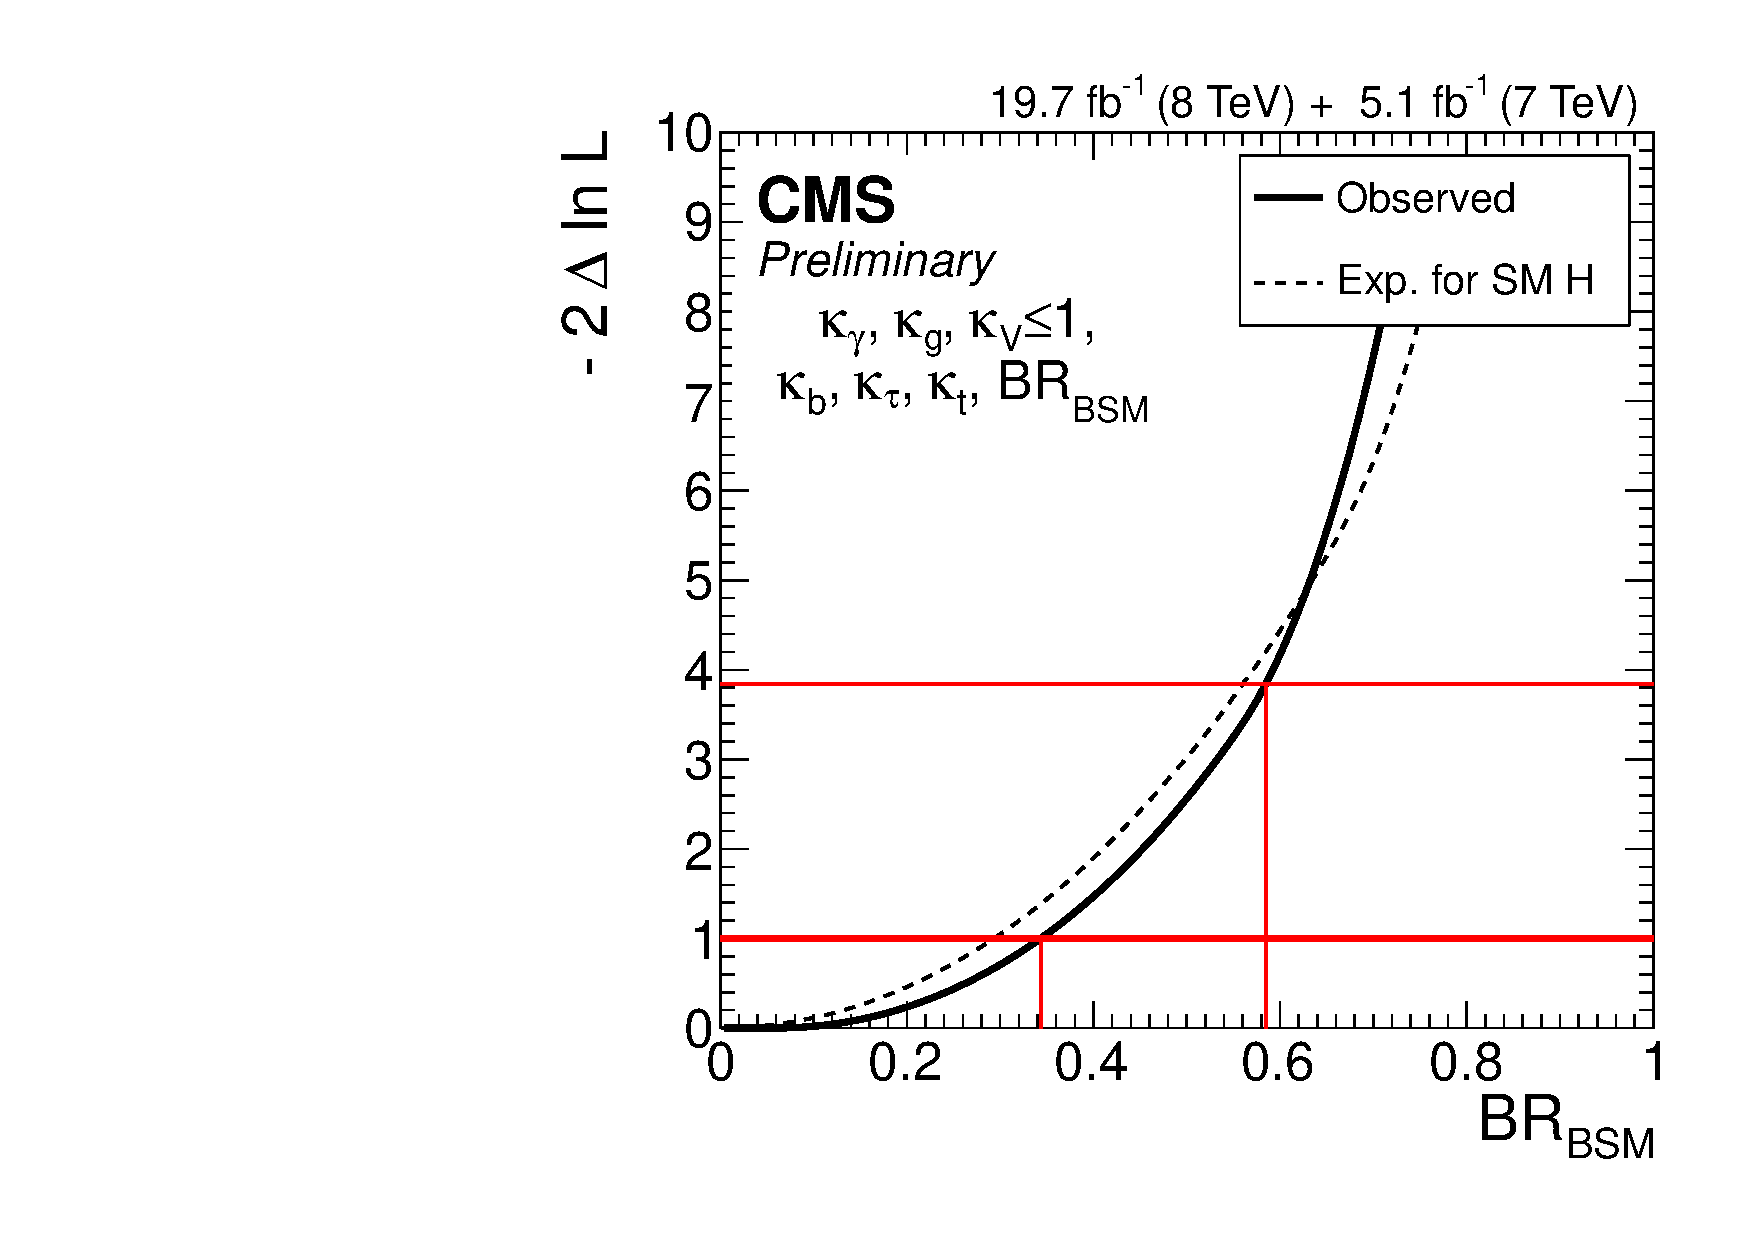
\includegraphics[height=.55\textheight]{TalkPics/panicpics/indirectbrbsm.pdf}
      \column{.05\textwidth}
    \end{columns}
    \begin{columns}
      \column{1.095\textwidth}
      \begin{block}{\scriptsize Theoretical motivation}
        \scriptsize
        \begin{itemize}
        \item Many BSM theories predict Higgs boson decays to invisible final states:
        \item[-] e.g. SUSY, extra dimensions, fourth-generation neutrinos
        \item These final state particles are often dark matter candidates
        \end{itemize}
      \end{block}
    \end{columns}

  \end{frame}

%OUTLINE
\begin{frame}
  \frametitle{Talk outline}
  \begin{columns}
    \column{.65\textwidth}
    \begin{block}{}
      \scriptsize
      \begin{itemize}
      \item For run 1 we had two sets of triggers
      \item[-] Prompt trigger used for current published result: HIG-13-30
      \item[-] Parked triggers analysis progress presented today
      \end{itemize}
    \end{block}
    \begin{block}{\footnotesize Overview}
      \scriptsize
      \begin{itemize}
      \item Reminder of prompt analysis
      \item Why we chose our new analysis strategy
      \item Details of parked analysis
      \item[-] Emphasis on changes from established prompt analysis
      \item Brief look at some other analysis techniques we are investigating
      \end{itemize}
    \end{block}
    \column{.45\textwidth}
    \vspace{0.7cm}

    \begin{fmfgraph*}(100,70)                                                                                                                              
        \fmfleft{i1,i2}                                                                                                                                   
        \fmfright{o1,o2,o3}                                                                                                                               
        \fmf{fermion}{i1,v1,o1}                                                                                                                           
        \fmf{fermion}{i2,v2,o3}                                                                                                                           
        \fmf{phantom,tension=4/5}{v1,v2}                                                                                                                  
        \fmffreeze                                                                                                                                        
        \fmf{photon,label=$W,,Z$}{v1,v3}                                                                                                                  
        \fmf{photon,label=$W,,Z$}{v2,v3}                                                                                                                  
        \fmf{dashes}{v3,o2}                                                                                                                               
        \fmflabel{$q$}{i1}                                                                                                                                
        \fmflabel{$q$}{i2}                                                                                                                                
        \fmflabel{$q$}{o1}                                                                                                                                
        \fmflabel{$q$}{o3}                                                                                                                                
        \fmflabel{$H$}{o2}                                                                                                                                
      \end{fmfgraph*}

    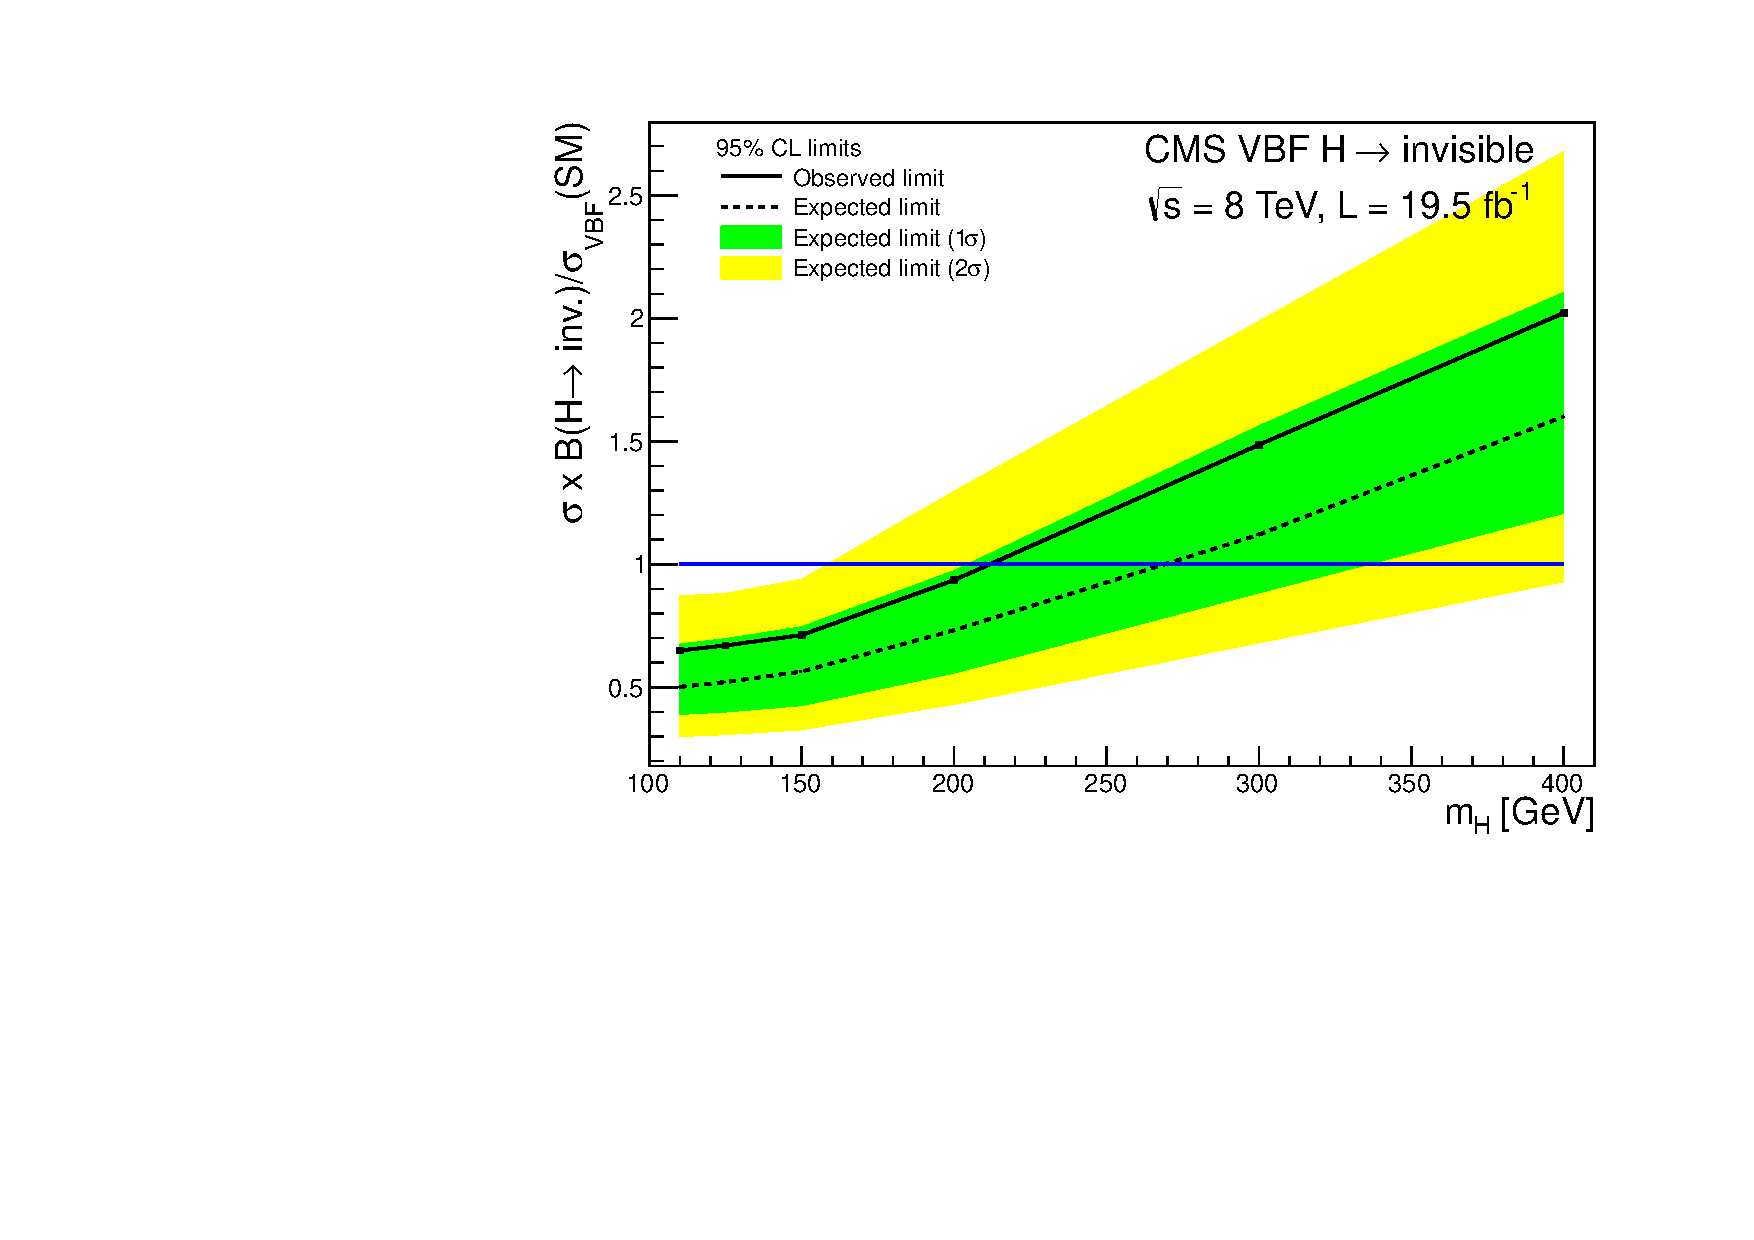
\includegraphics[width=\textwidth]{TalkPics/hig1330approval/vbflimit.pdf}
    \end{columns}
\end{frame}

\begin{frame}
  \frametitle{Prompt Analysis}
  \begin{columns}
    \column{.5\textwidth}
    \begin{block}{}
      \scriptsize
      \begin{itemize}
      \item Single bin counting experiment
      \item[-] Signal region chosen to eliminate QCD and be above trigger turn ons
      \item Major backgrounds use data driven estimates:
      \item $Z\rightarrow\nu\nu$,$W\rightarrow\ell\nu$, QCD
      \item Minor backgrounds taken from MC:
      \item VV, W$\gamma$, $t\bar{t}$, single top
      \item Expected limit 49\% at $m_{H}=125$ GeV
      \end{itemize}
    \end{block}
    \column{.5\textwidth}
    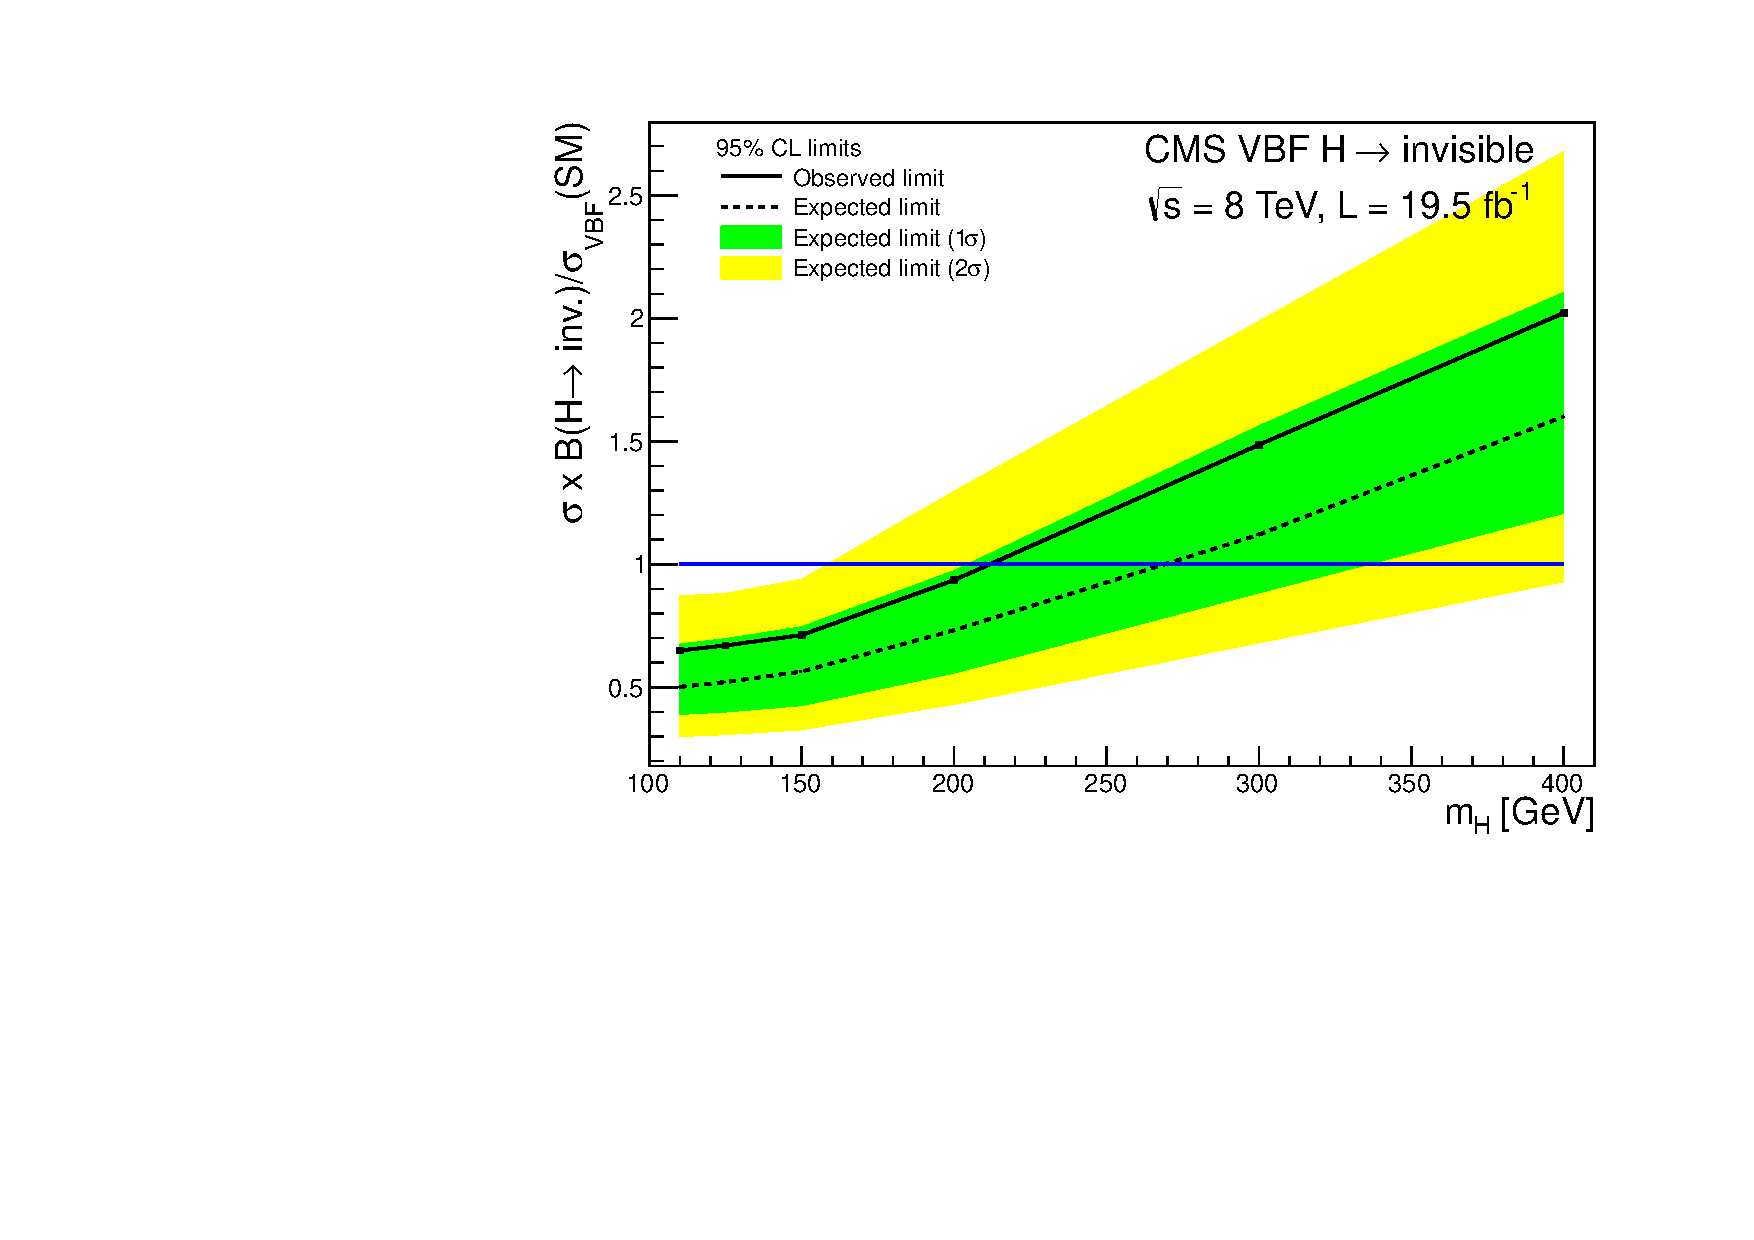
\includegraphics[width=\textwidth]{TalkPics/hig1330approval/vbflimit.pdf}
  \end{columns}
  \begin{columns}
    \column{1.05\textwidth}
  \begin{block}{\scriptsize Data driven background estimation}
    \begin{columns}
      \column{.35\textwidth}
      \scriptsize
     W: $N_{S}=N_{S}^{MC}\frac{N_{C}^{Data}-N_{C}^{Bkg}}{N_{C}^{MC}}$
     \column{.55\textwidth}
     \scriptsize  
   Z: $N_{S}^{Z\rightarrow\nu\nu}=\left(N_{C}^{Data}-N_{C}^{bkg}\right) \cdot\frac{\sigma\left(Z\rightarrow\nu\nu\right)}{\sigma\left(Z\rightarrow\mu\mu\right)}\cdot \frac{\epsilon_{S}^{ZMC}}{\epsilon_{C}^{ZMC}}$
       \end{columns}
  \end{block}
  \end{columns}
\end{frame}

\begin{frame}
  \frametitle{Parked Triggers}
  \begin{block}{}
      \scriptsize
    \begin{itemize}
    \item Use already analysed prompt trigger for run A
    \item One parked trigger for runs B and C, another for run D
    \item All parked and prompt triggers are seeded by L1ETM40
    \item Parked triggers have looser HLT thresholds
    \item This allows us to look at new regions of phase space and different analysis techniques
    \end{itemize}
  \end{block}
  \begin{block}{}
    \scriptsize
    \centering
    \begin{tabular}{|l|c|c|c|}
      \hline
      Run period & MET cut & dijet $p_{T}$ cut & dijet mass cut \\
      \hline
      A & METnoMuons$>$65 GeV & DiPFJet40 & MJJ800 \\
      B\&C & N/A & DiJet35 & MJJ700 \\
      D & N/A & DiJet30 & MJJ700 \\
      \hline
    \end{tabular}
  \end{block}
\end{frame}

%FRAMEWORK STRATEGY AND SYNC
\begin{frame}
  \frametitle{Software framework strategy}
  \begin{block}{\scriptsize Prompt analysis}
    \scriptsize
    \begin{itemize}
    \item Two frameworks: Analyses A and B
    \item independent ntuples and analysis code
    \end{itemize}
  \end{block}
  \begin{block}{\scriptsize Parked analysis}
      \scriptsize
      \begin{itemize}
      \item Insufficient manpower to maintain and develop two frameworks
      \item Moved to one fully developed framework rather than two underdeveloped ones
      \item[-] New framework uses analysis B ntuples
      \item Synchronised yields in signal and control regions between new framework and old analyses A and B
      \item Repeated expected limit calculation from HIG-13-030 analysis with the new framework and parked data
      \item[-] Agrees with HIG-13-030 to within 2\%, which is good given rereco, and change of global tag and triggers
      \end{itemize}
  \end{block}
\end{frame}


%DIFFERENT OPTIONS AND WHY WE CHOSE WHAT WE DID
\begin{frame}
  \frametitle{Analysis strategy}
  \begin{block}{\scriptsize Initial plan}
    \scriptsize
    \begin{itemize}{}
    \item Define a loose pre-selection and model QCD shape
    \item Several options for analysis strategy:
    \item[-] Rectangular cuts and counting experiment
    \item[-] Rectangular cuts and shape experiment
    \item[-] MVA and counting experiment
    \item[-] MVA and shape experiment
    \end{itemize}
  \end{block}
  \begin{block}{\scriptsize Final plan for parked data}
    \begin{itemize}
      \scriptsize
    \item Unable to model QCD shape - details later
    \item Altered signal region cuts to remove QCD
    \item Remaining backgrounds very signal like in variables studied so far
    \item[-] Opted for cut and count analysis
    \end{itemize}
  \end{block}
\end{frame}

%CHECK LIST UP TO DATE
\begin{frame}
  \frametitle{Changes since prompt analysis}
  \begin{block}{\scriptsize Trigger}
    \scriptsize
    \begin{itemize}
    \item Parked trigger efficiency has been measured including variable correlation
    \item[-] This allows the trigger turn on region to be used
      \end{itemize}
    \end{block}
  \begin{block}{\scriptsize Signal region}
    \scriptsize
    \begin{itemize}
    \item The signal region has been reoptimised for the looser parked triggers
    \item[-] New region uses new variable has higher signal efficiency with less QCD
    \end{itemize}
  \end{block}
\begin{block}{\scriptsize Background estimation}
  \scriptsize
  \begin{itemize}
    \item A top control region has been added
    \item Minor modifications made to $W\rightarrow\tau\nu$ background estimation method
    \item QCD background estimation method changed
    \item W$\gamma$ contribution found to be modelled already by our $W\rightarrow\ell\nu$ Monte Carlo
    \end{itemize}
  \end{block}
\end{frame}

%TRIGGER EFFICIENCY
\begin{frame}
  \frametitle{Trigger efficiency}
  \begin{columns}
    \column{.55\textwidth}
    \begin{block}{}
      \scriptsize
      \begin{itemize}
      \item The variables used in prompt and parked triggers are highly correlated:
      \item[-] dijet mass, METnoMU, jet 2 $p_{T}$
      \item In the prompt analysis we neglected correlations and cut to ensure trigger was $>95\%$ efficient
      \item For the parked analysis we use a 2D binning in dijet mass and jet 2 $p_{T}$
      \item[-] MJJ: 0,600,800,900,1000,5000
      \item[-] Jet 2 $p_{T}$: 30,40,50,60,1000
      \item In each bin we fit the METnoMU trigger turn on using an error function
      \item We then combine the turn ons from runs A, BC and D weighted by luminosity and apply this to MC events

      \end{itemize}
    \end{block}
    \column{.5\textwidth}
    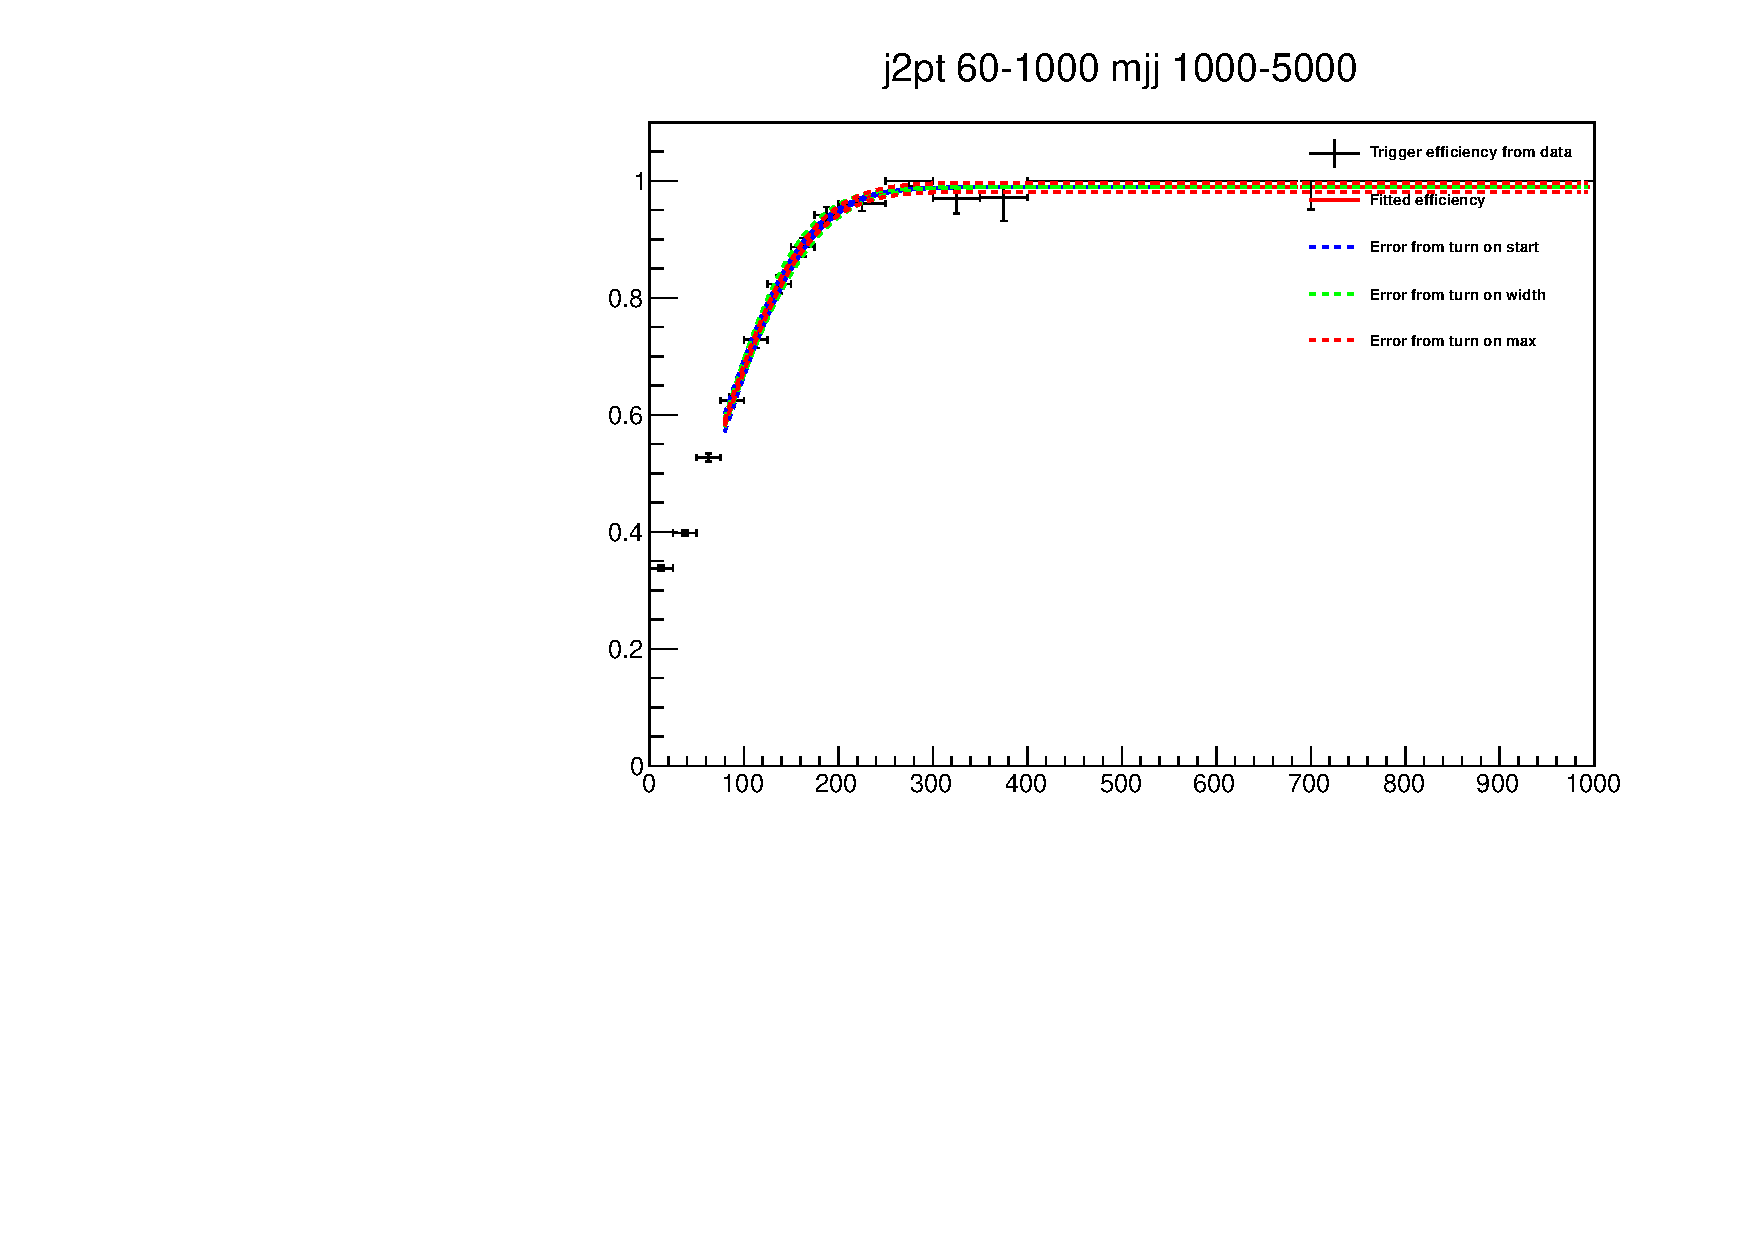
\includegraphics[width=1.1\textwidth]{TalkPics/higgsexo031114/trigfitplots/hData_MET_1D_45D.pdf}
    \vspace{-.2cm}

    \hfill \scriptsize METnoMU/GeV
  \end{columns}
\end{frame}

\begin{frame}
  \frametitle{QCD issues}
  \begin{block}{}
    \scriptsize Several methods tried to model QCD
  \end{block}
  \begin{block}{\scriptsize Standard MC}
    \scriptsize
    \begin{itemize}
    \item[-] doesn't have enough events
    \end{itemize}
  \end{block}
  \begin{block}{\scriptsize Private VBF enriched QCD MC sample}
    \scriptsize
    \begin{itemize}
    \item[-] Can only enrich in events with real met
    \item[-] Can't model met from mismeasurement
    \end{itemize}
  \end{block}
  \begin{block}{\scriptsize Data-driven shape using different jet pairs in the event}
    \scriptsize
    \begin{itemize}
    \item[-] Jet kinematics are very biased
    \item[-] Ordering in $p_{T}$ and angle have been tried
    \item[-] Reweighting individual distributions to fix others has been tried
    \end{itemize}
  \end{block}
\end{frame}

\begin{frame}
  \frametitle{Preselection choice}
  \vspace{-.4cm}
  \begin{columns}
    \column{1.05\textwidth}
  \begin{block}{}
    \scriptsize
    \begin{itemize}
    \item Trigger turn ons and detector acceptance impose the following cuts:
    \item[-] $\eta_{j1} \cdot \eta_{j2}<0,\, \eta_{j1,2}<4.7,\, \text{jet\,1}\, p_{T}>50 \,\text{GeV},\, \Delta\eta_{jj}>3.6,$\\$\, \text{jet\,2}\, p_{T}>40 \,\text{GeV},\text{METnomu}>90\,\text{GeV},\, M_{jj}>800 \,\text{GeV}$
    \item As in the prompt analysis we also veto events with 'veto' electrons or muons
    \item Poor data-MC agreement from QCD contamination motivates the following additional cuts:
    \item $\frac{METnomu}{\sigma_{METnomu}}>3.0,\,\text{Min}\Delta\phi(all\,jets\,p_{T}>30\,GeV,METnomu)>1.0,\,M_{jj}>1000\,\text{GeV}$
    \end{itemize}
  \end{block}
  \end{columns}
  \begin{columns}
    \column{1.15\textwidth}
  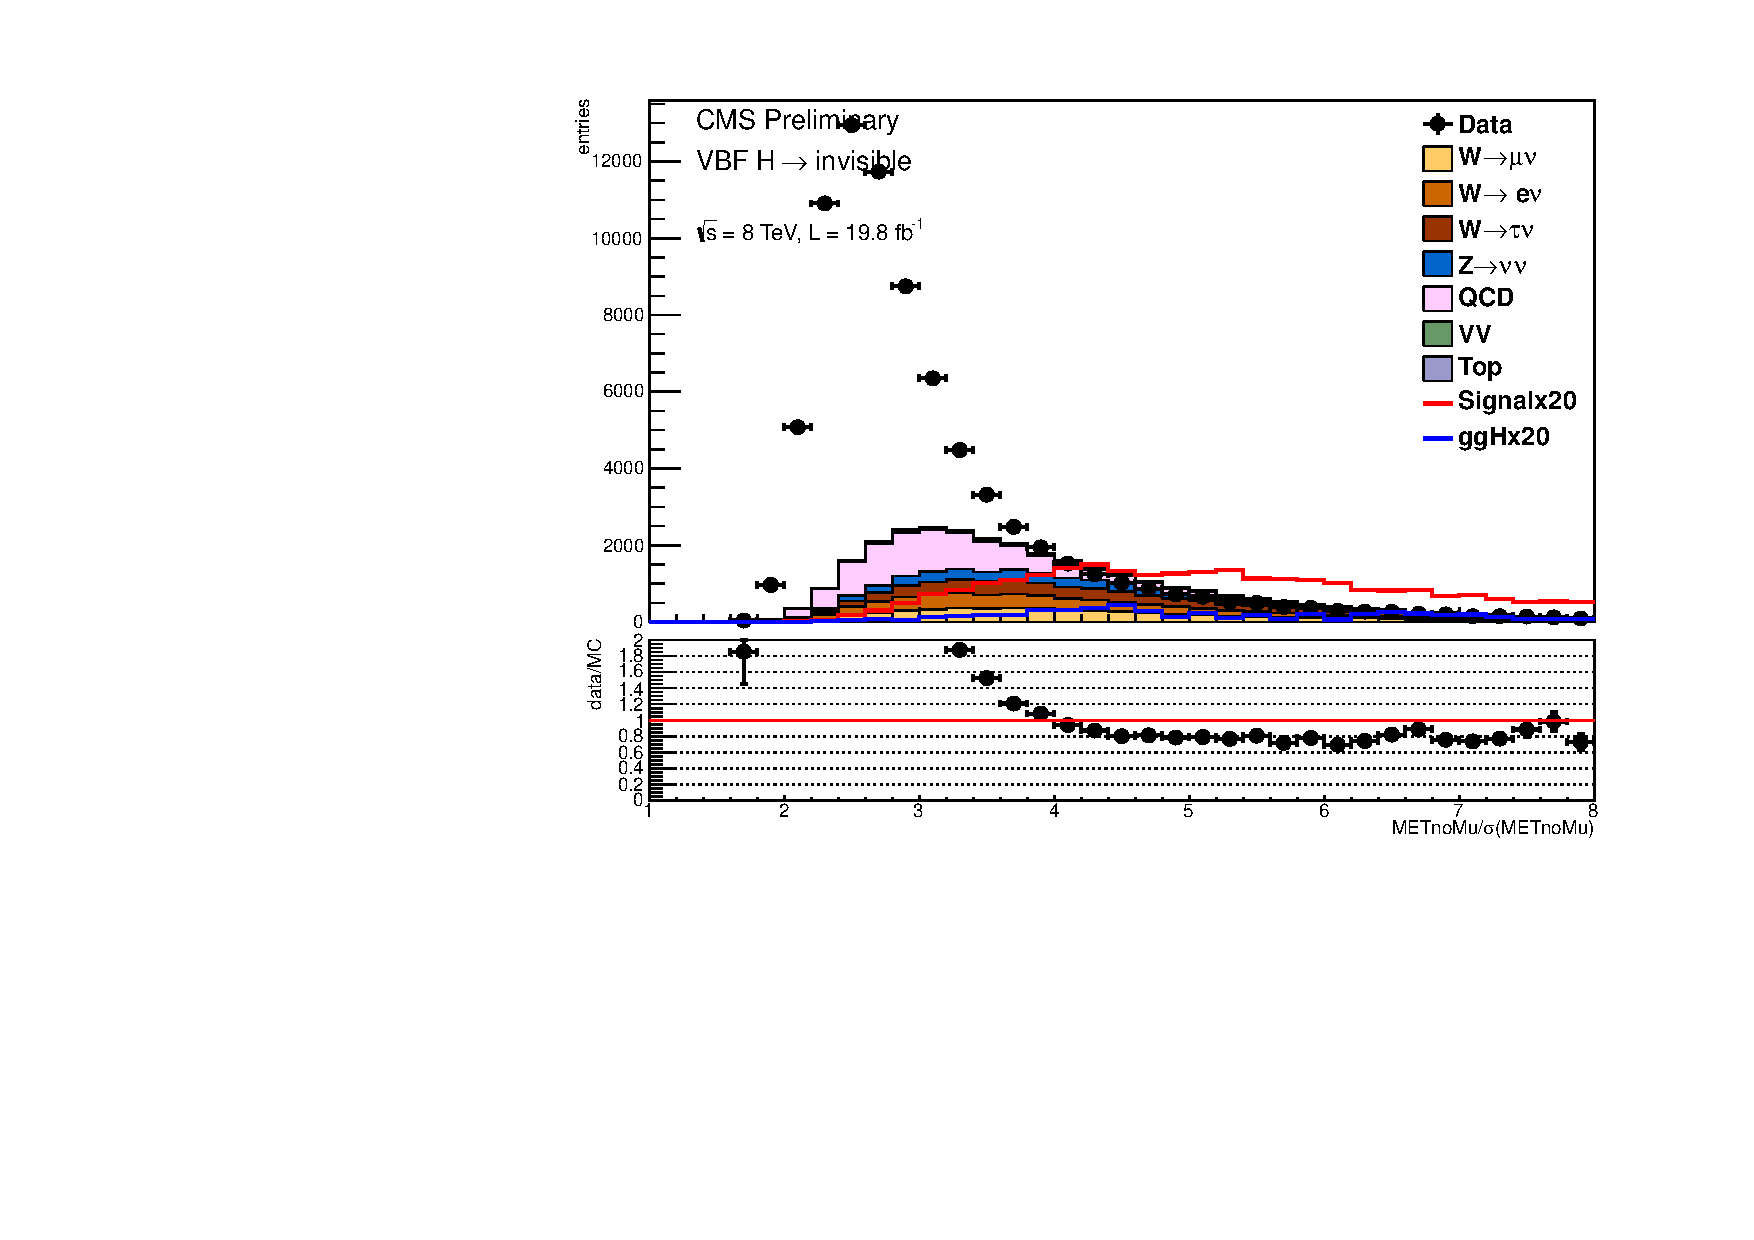
\includegraphics[width=.34\textwidth]{TalkPics/higgsexo031114/nopreselnunu_metnomu_significance.pdf}
  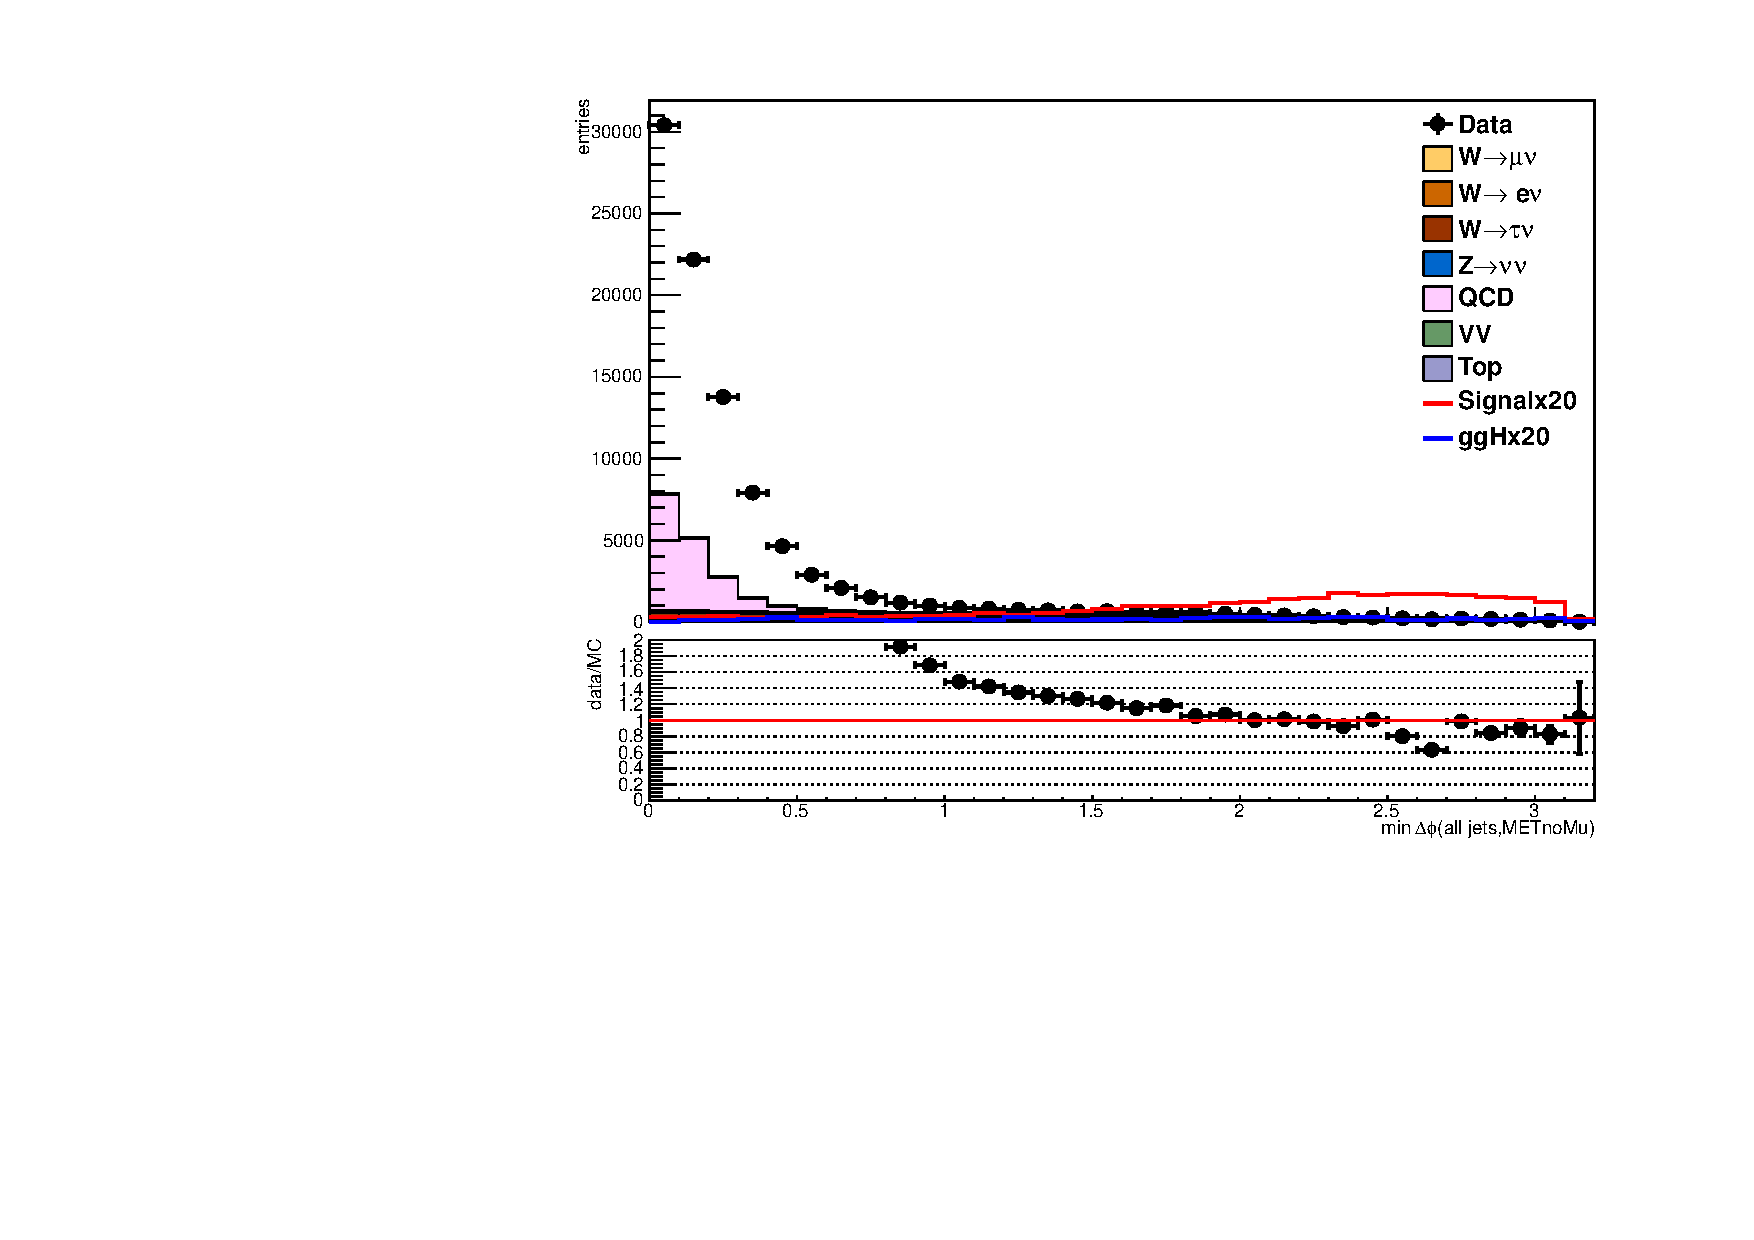
\includegraphics[width=.34\textwidth]{TalkPics/higgsexo031114/metsigpreselnunu_alljetsmetnomu_mindphi.pdf}
  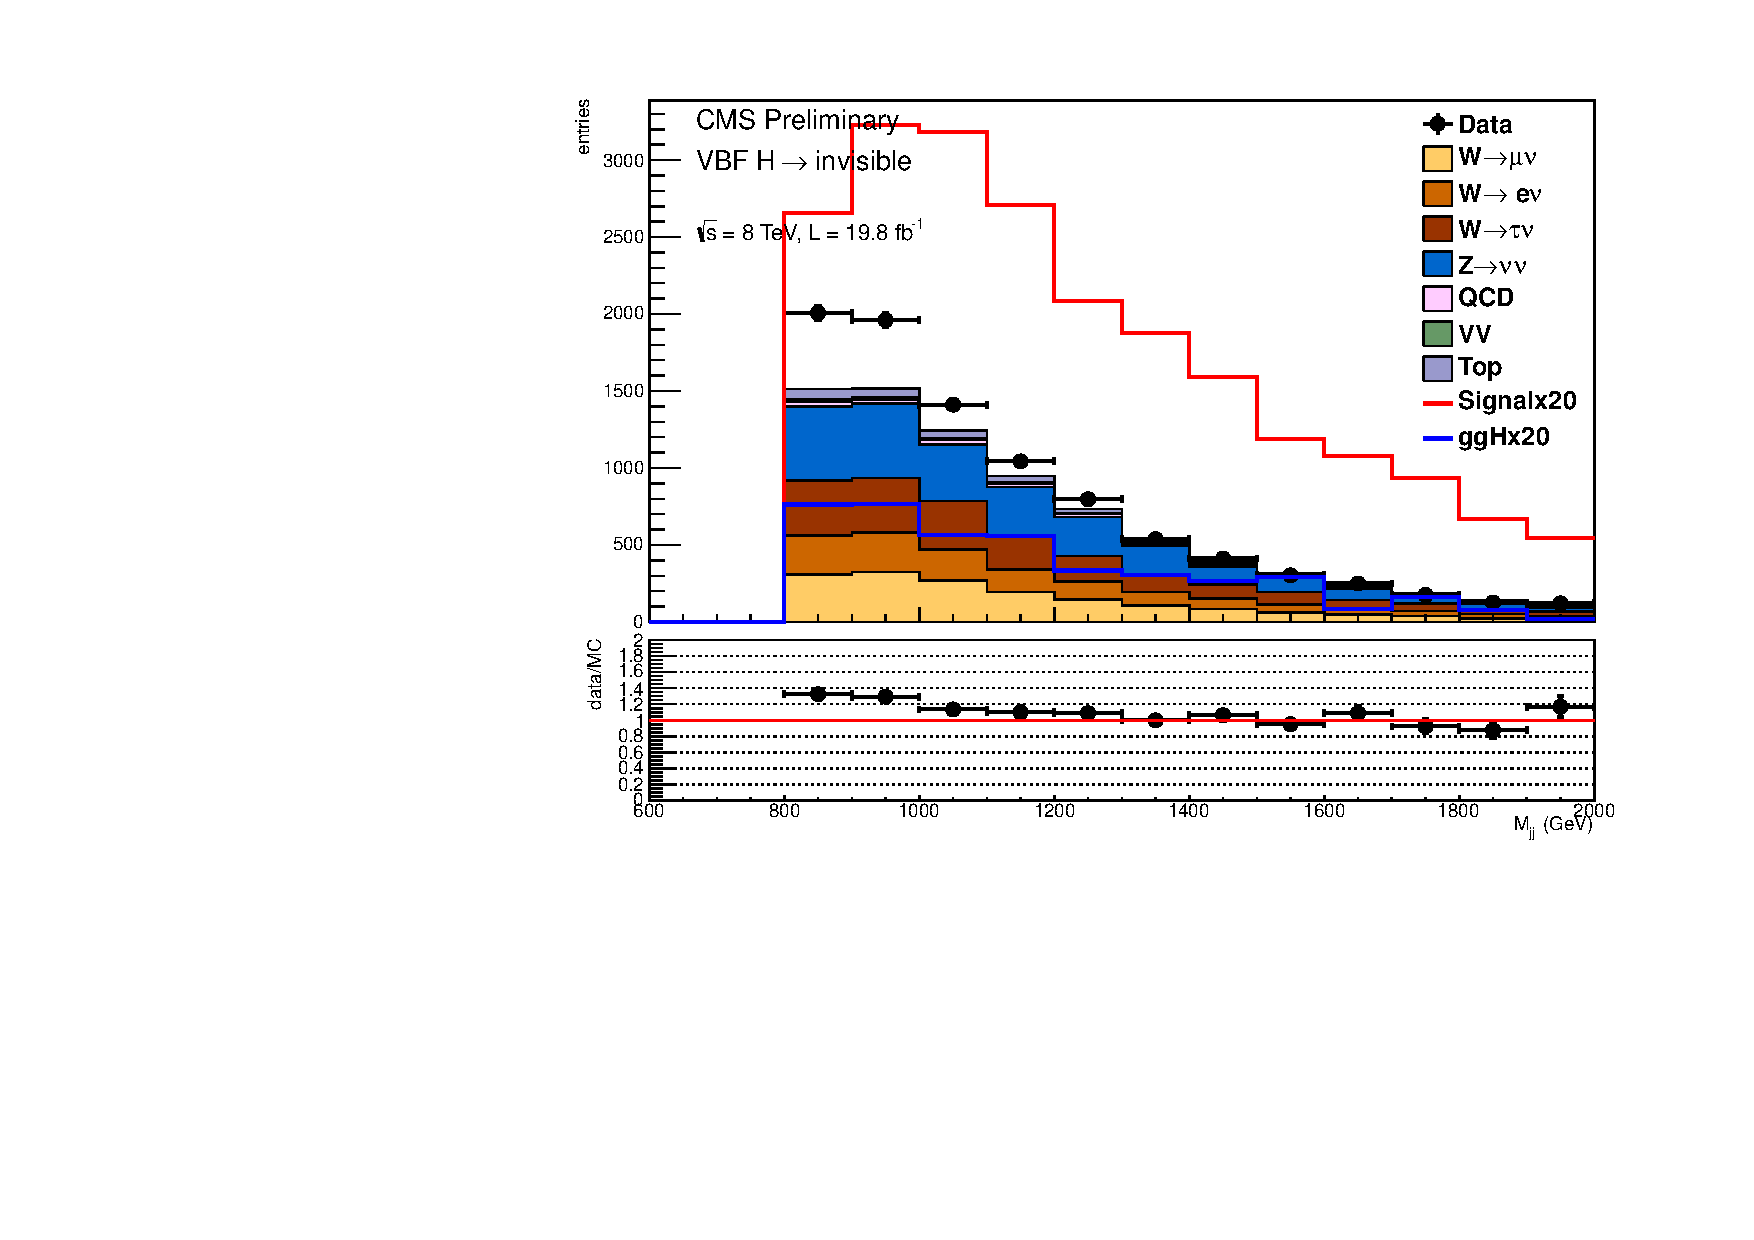
\includegraphics[width=.34\textwidth]{TalkPics/higgsexo031114/mjj800nunu_dijet_M.pdf}
  \end{columns}
\end{frame}

%SIGNAL SELECTION TAKE AN PLOTS
\begin{frame}
  \frametitle{Signal region selection}
   \begin{columns}
     \column{.55\textwidth}
     \begin{block}{}
       \scriptsize
       \begin{itemize}
       \item Can't model QCD shape so alter cuts to remove most QCD
       \item[-] Can then tolerate a larger uncertainty on QCD estimation
       \item[-] QCD in plots is vbf enriched MC doesn't model all QCD
       \item Agreement in control regions is good for $\frac{METnoMU}{\sigma_{METnoMU}}>4$ and $\text{Min}\Delta\phi(all\,jets,METnomu)>2.0$
       \item Signal contribution also large for some regions of parameter space
       \item We blind the data in this region and use it as a basis for signal region optimisation
       \end{itemize}
    \end{block}
    \column{.5\textwidth}
    \vspace{-.25cm}

    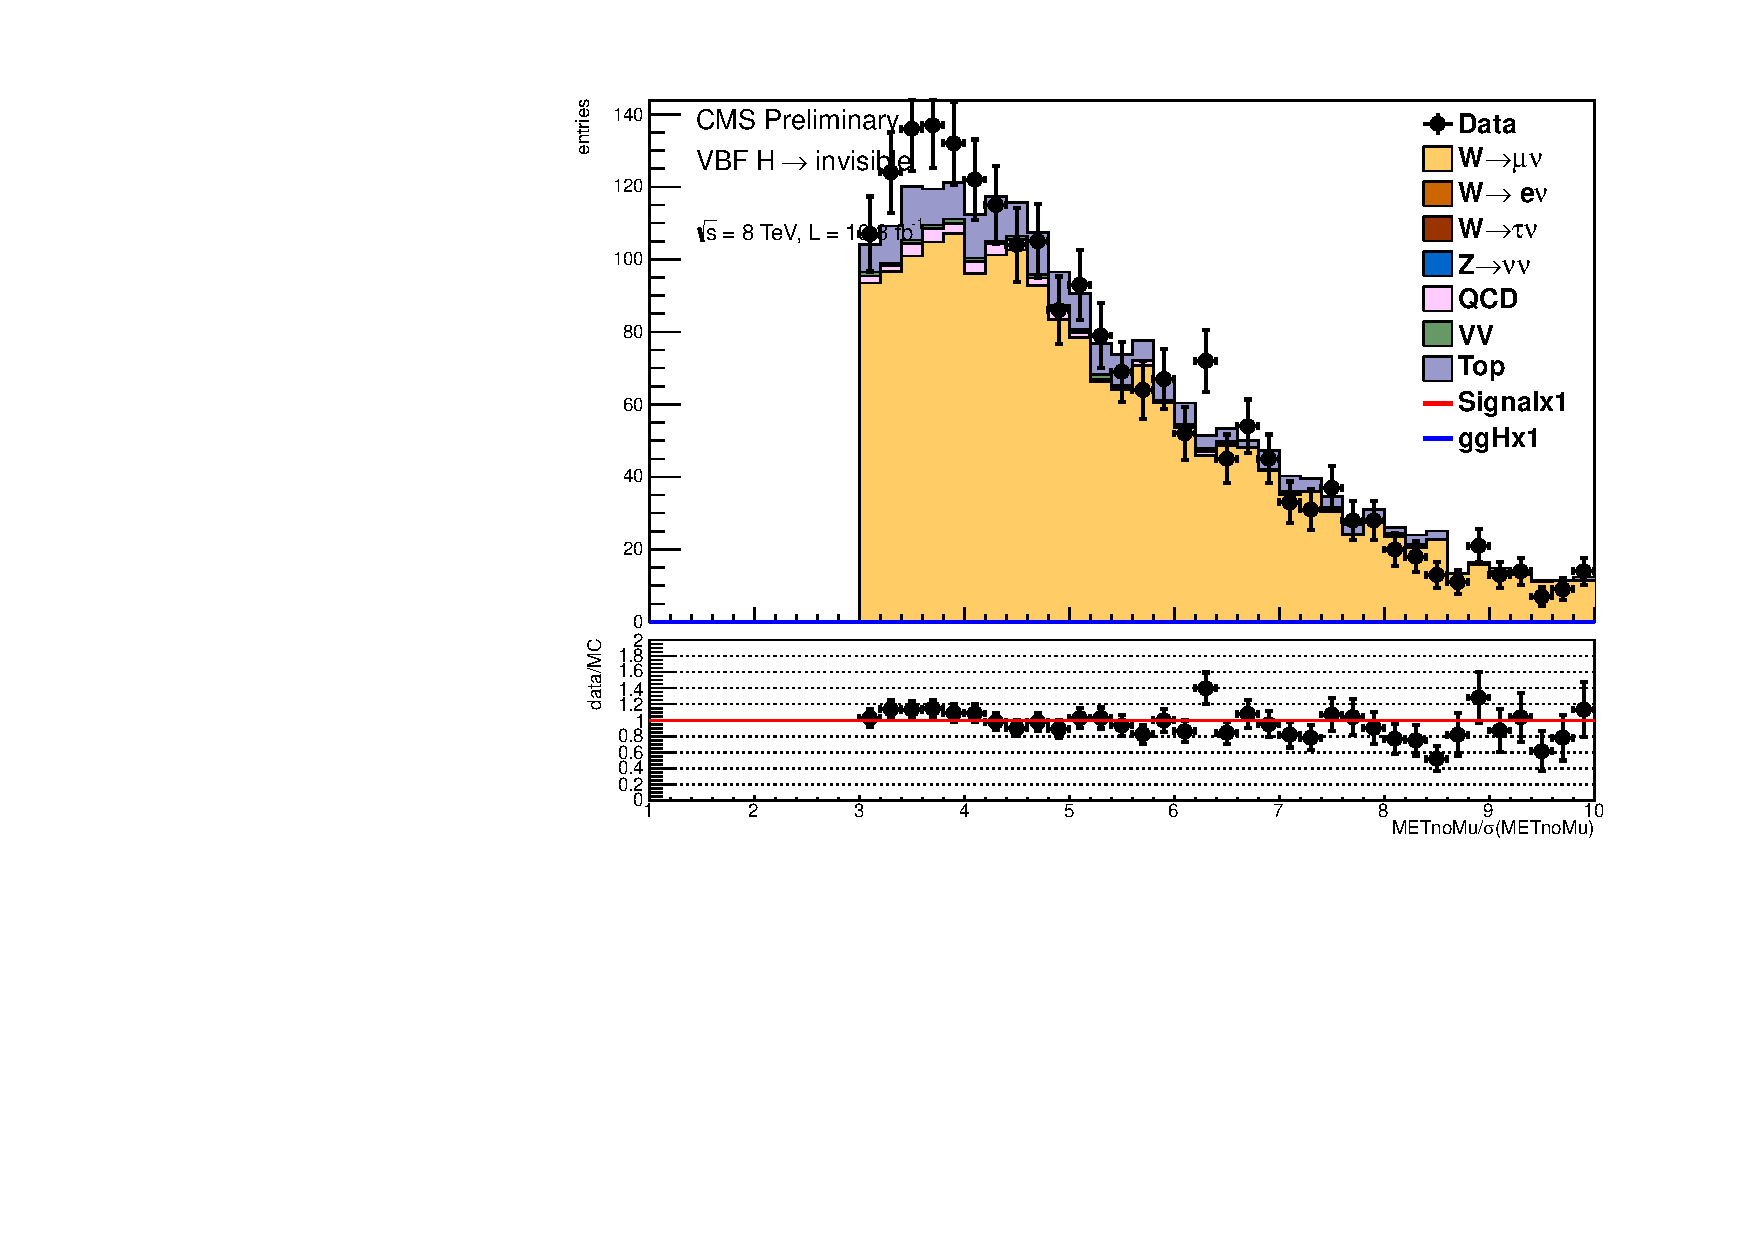
\includegraphics[clip=true,trim=0 0 0 20,width=.95\textwidth]{TalkPics/higgsexo031114/output_presel/munu_metnomu_significance.pdf}
    \vspace{-.05cm}
    

    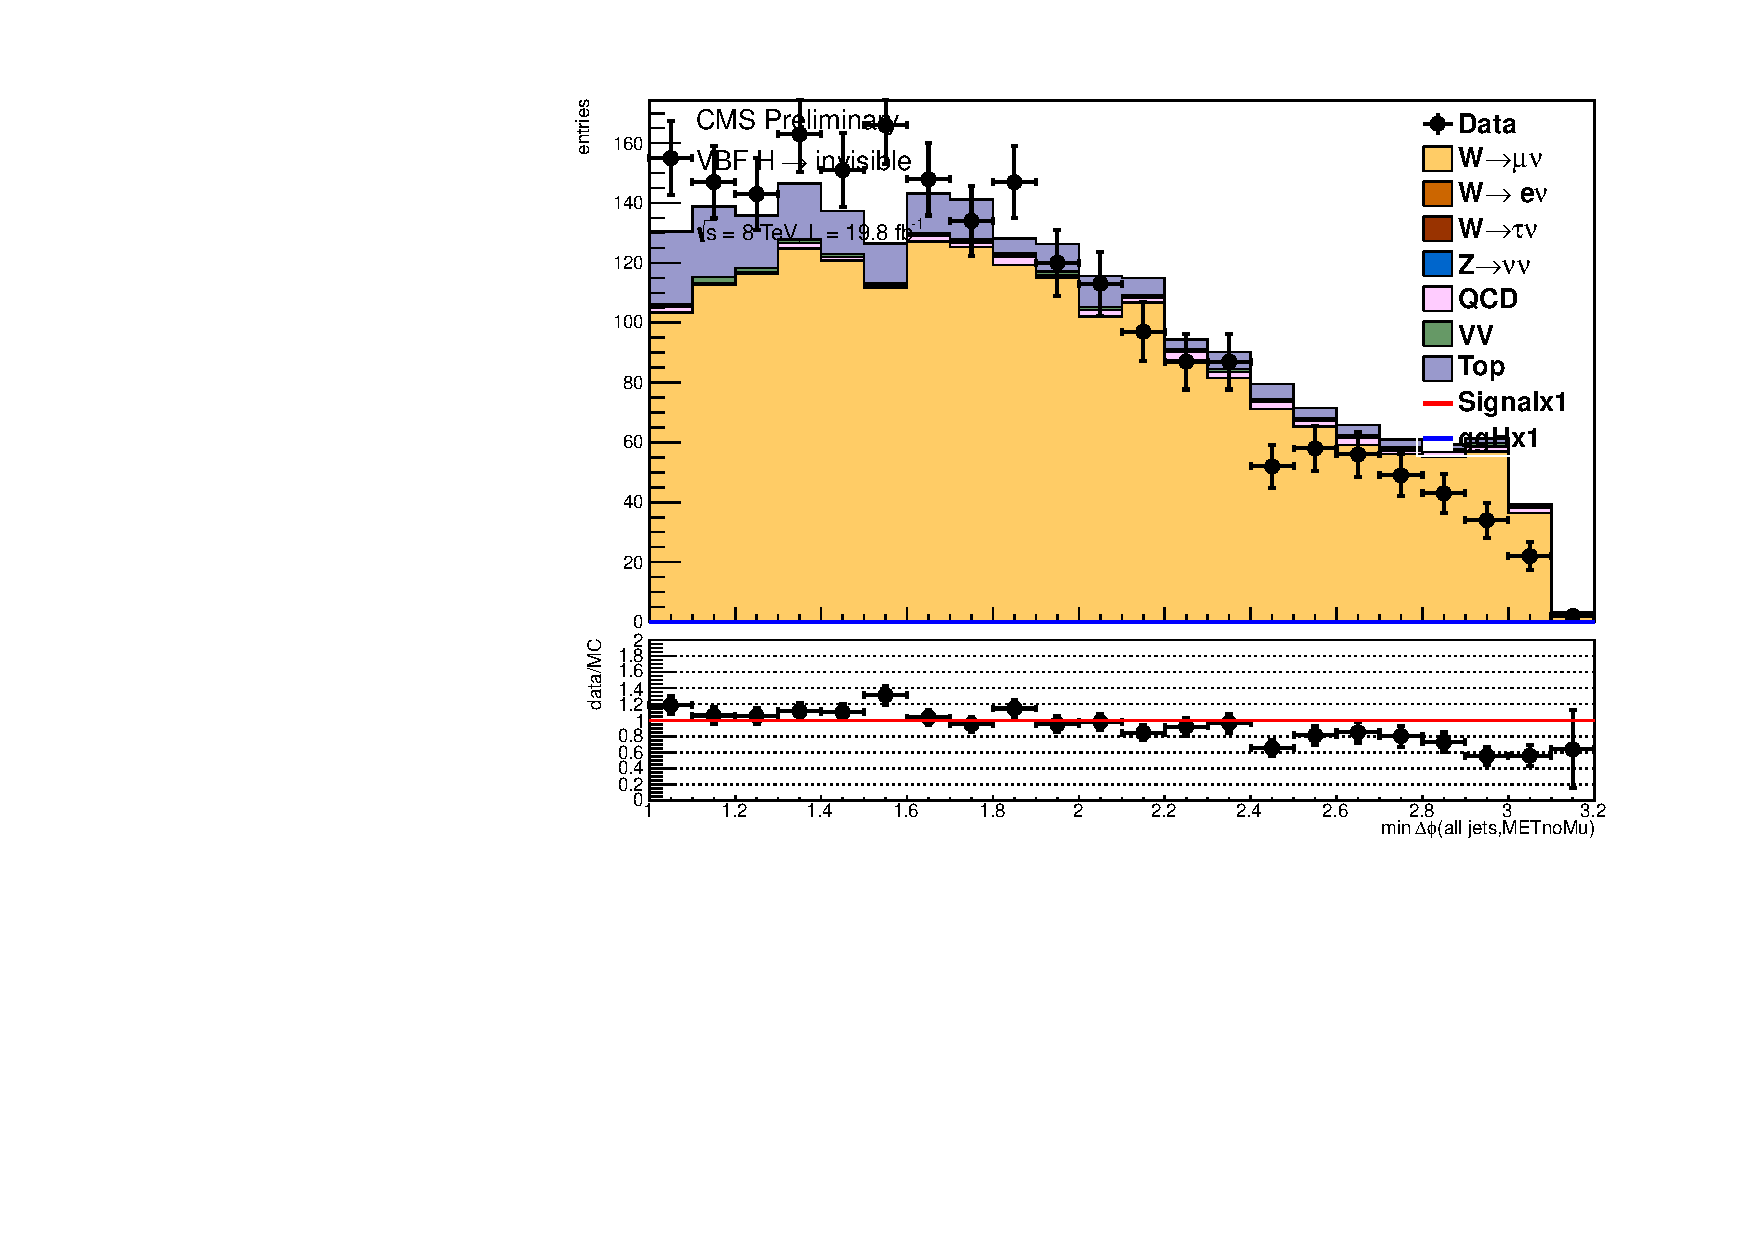
\includegraphics[clip=true,trim=0 0 0 20,width=.95\textwidth]{TalkPics/higgsexo031114/output_presel/munu_alljetsmetnomu_mindphi.pdf}
  \end{columns}
\end{frame}

\begin{frame}
  \frametitle{Signal region selection}
   \begin{columns}
     \column{.55\textwidth}
     \begin{block}{}
       \scriptsize
       \begin{itemize}
       \item We optimise by choosing the cut values with the best 95\% C.L. expected limit
       \item[-] Limit calculation details later
       \item We scanned through jet 2 $p_{T}$, dijet mass and $\text{Min}\Delta\phi(all\,jets\,,METnomu)$
       \item Best limit was found for:
       \item[-] No additional jet 2 $p_{T}$ cut
       \item[-] $\frac{METnoMU}{\sigma_{METnoMU}}>4$
       \item[-] $\text{Min}\Delta\phi(all\,jets,METnomu)>2.5$
       \item Discrepancy outside signal region is from QCD
       \item This was used as our ``signal region''
       \end{itemize}
    \end{block}
    \column{.5\textwidth}
    \vspace{-.25cm}

    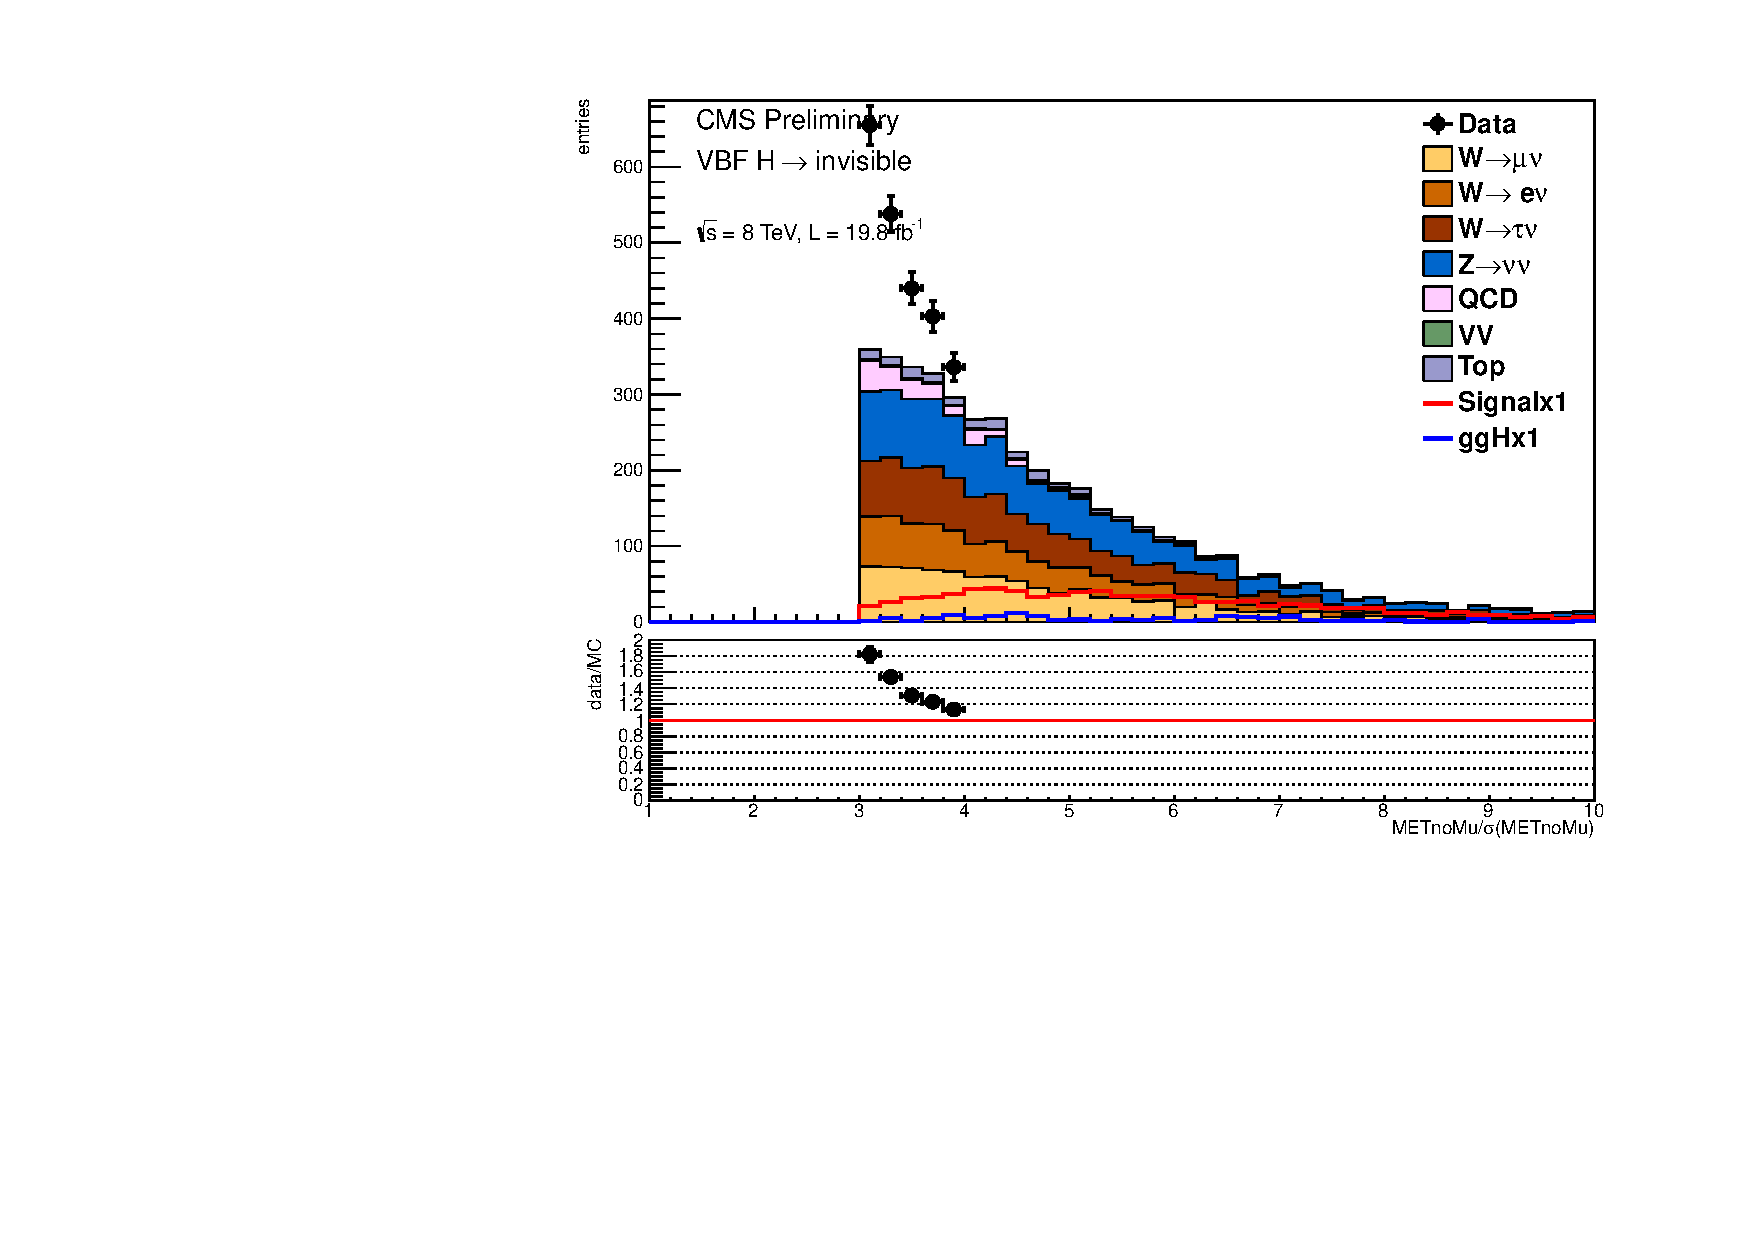
\includegraphics[clip=true,trim=0 0 0 20,width=.95\textwidth]{TalkPics/higgsexo031114/output_presel/nunu_metnomu_significance.pdf}
    \vspace{-.05cm}
    

    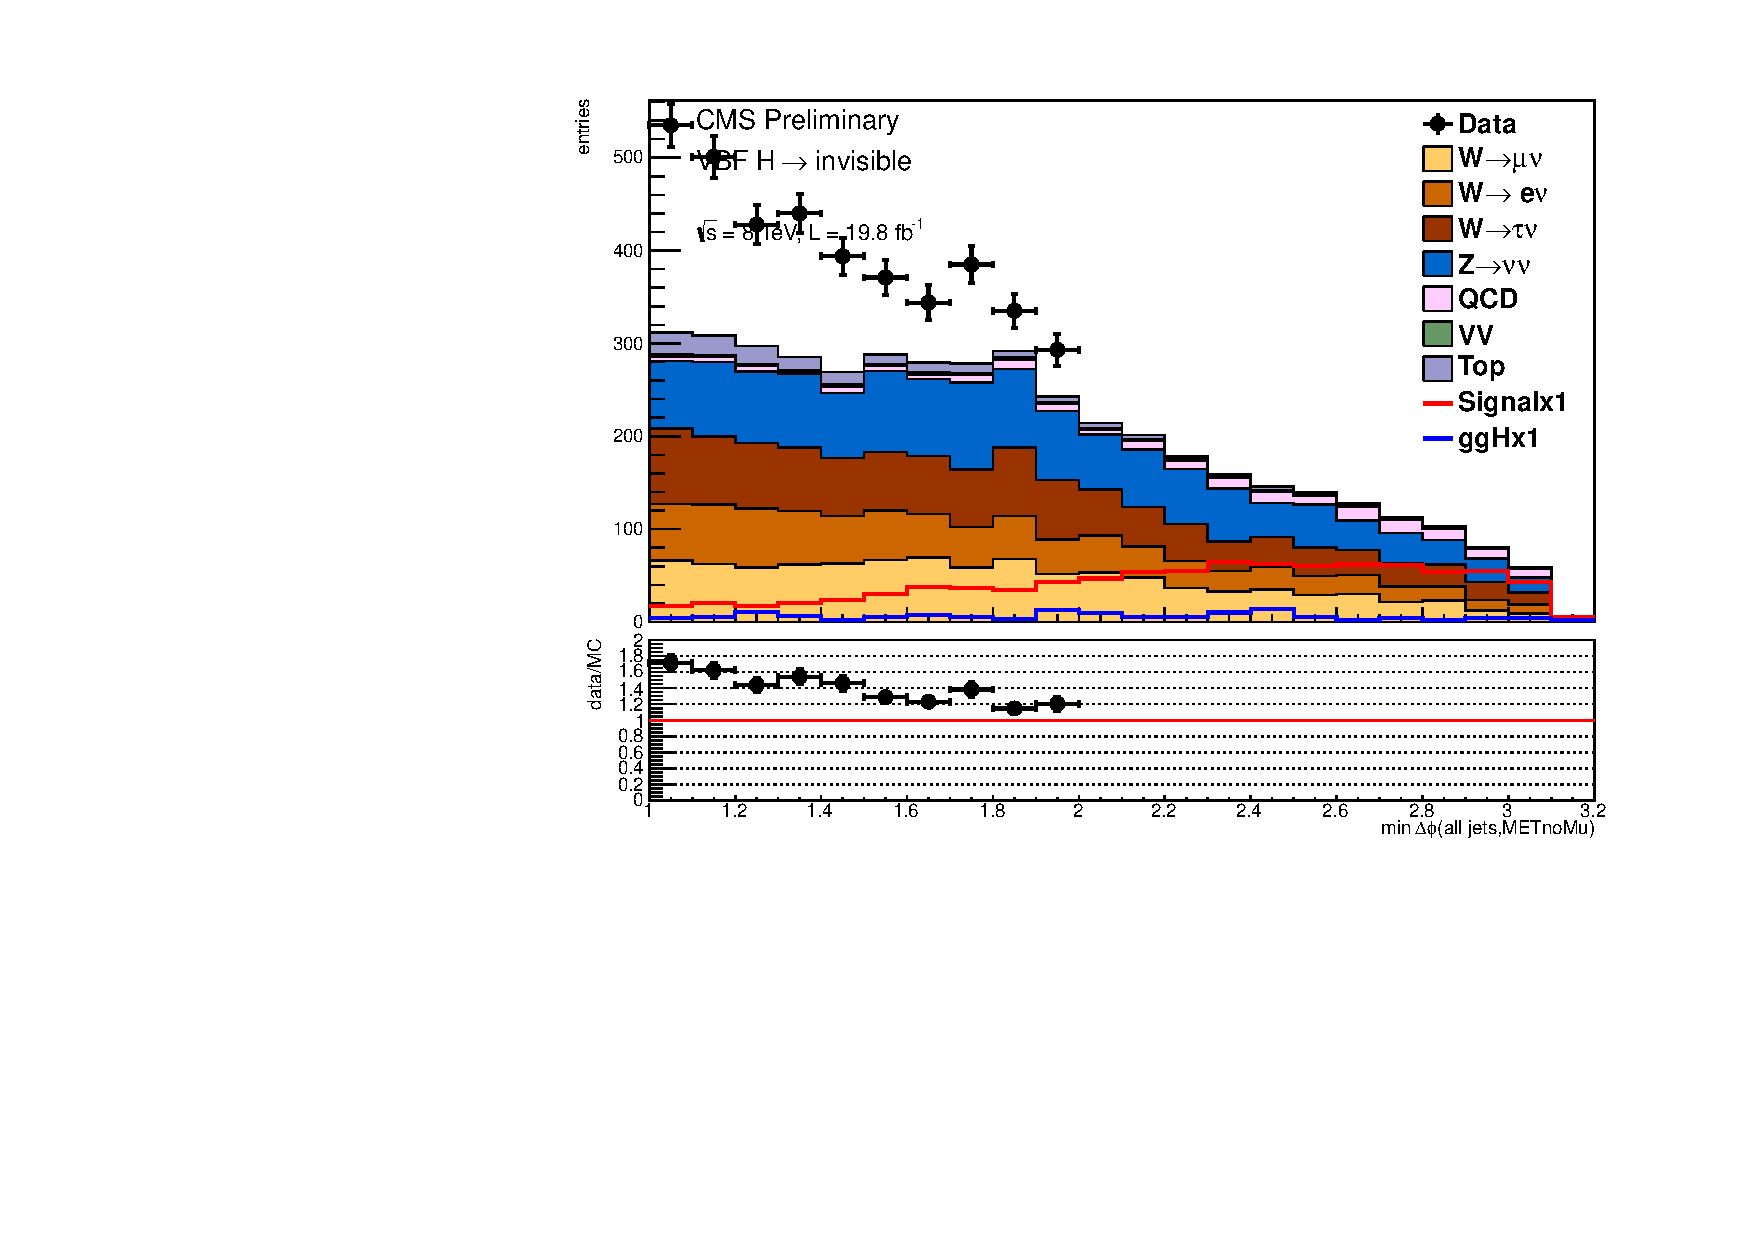
\includegraphics[clip=true,trim=0 0 0 20,width=.95\textwidth]{TalkPics/higgsexo031114/output_presel/nunu_alljetsmetnomu_mindphi.pdf}
  \end{columns}
\end{frame}

%TOP CONTROL REGION
\begin{frame}
  \frametitle{Top control region}
  \begin{columns}
    \column{.55\textwidth}
    \begin{block}{}
      \scriptsize
      \begin{itemize}
      \item Top contribution to V+jets control regions is non-negligible
      \item[-] up to 16\% in $W\rightarrow\tau\nu$
      \item Use method used for W backgrounds in prompt analysis
      \item Region: signal region with lepton veto replaced with requirement for 1 tight muon and 1 tight electron
      \item[-] Very few events in $e\mu$ region so also removed $\text{Min}\Delta\phi(all\,jets,\,METnomu)$ cut
      \end{itemize}
      \begin{tabular}{|l|c|}
        \hline
        $N_{C}^{data}$ & $28\pm 5.3 (\text{stat.})$\\
        $N_{C}^{bkg}$ & $0.6\pm 0.2 (\text{MC stat.})$  \\
        $N_{S}^{top\,MC}$ & $9.6\pm 1.8 (\text{MC stat.})$ \\
        $N_{C}^{top\,MC}$ & $42.6\pm 5.2 (\text{MC stat.})$   \\
        \hline
        $N_{S}^{top}$ & \textcolor{red}{$6.1\pm 1.2 (\text{stat.}) \pm 1.4 (\text{MC stat.})$} \\
        \hline
\end{tabular}
    \end{block}
    \column{.5\textwidth}
    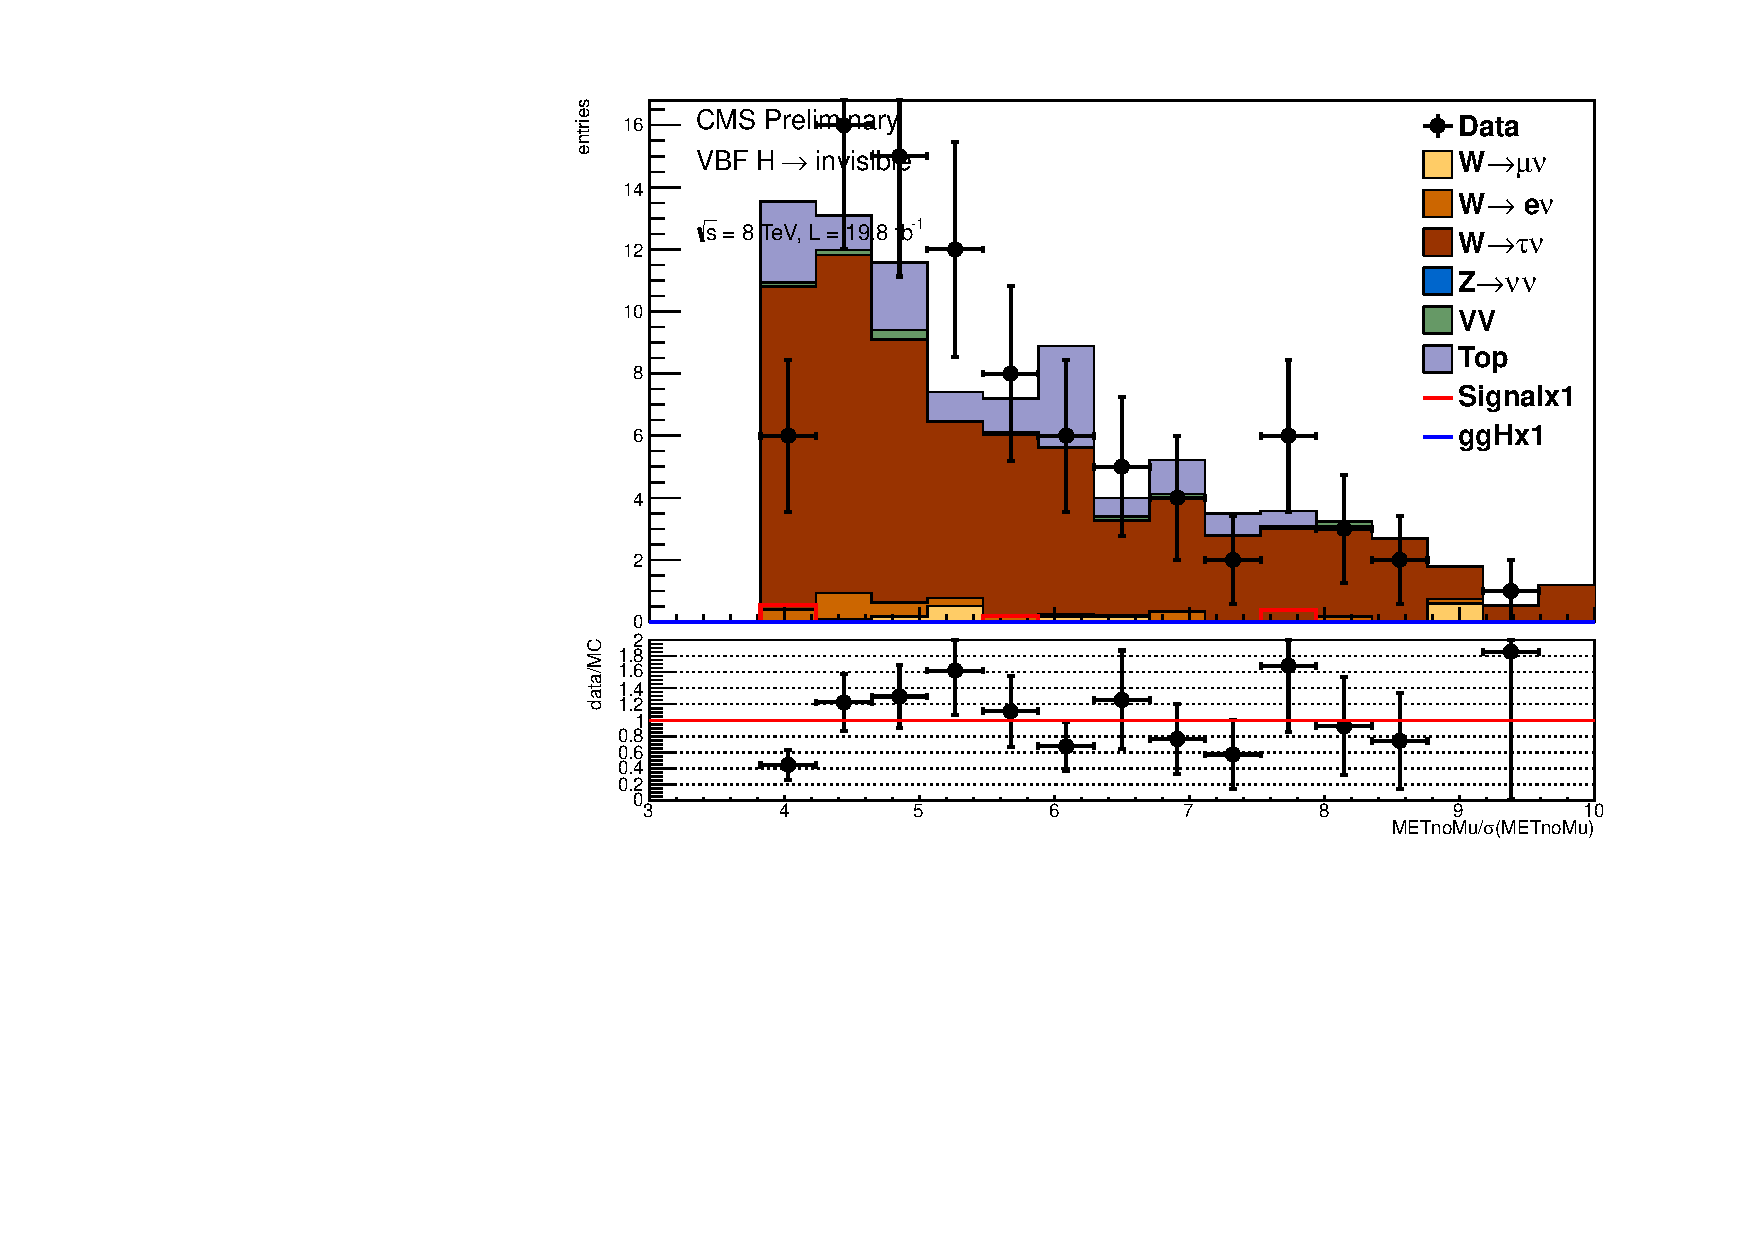
\includegraphics[clip=true,trim=0 100 0 0,width=\textwidth]{TalkPics/higgsexo031114/output_sigreg/taunu_metnomu_significance.pdf}
    \vspace{-.3cm}

    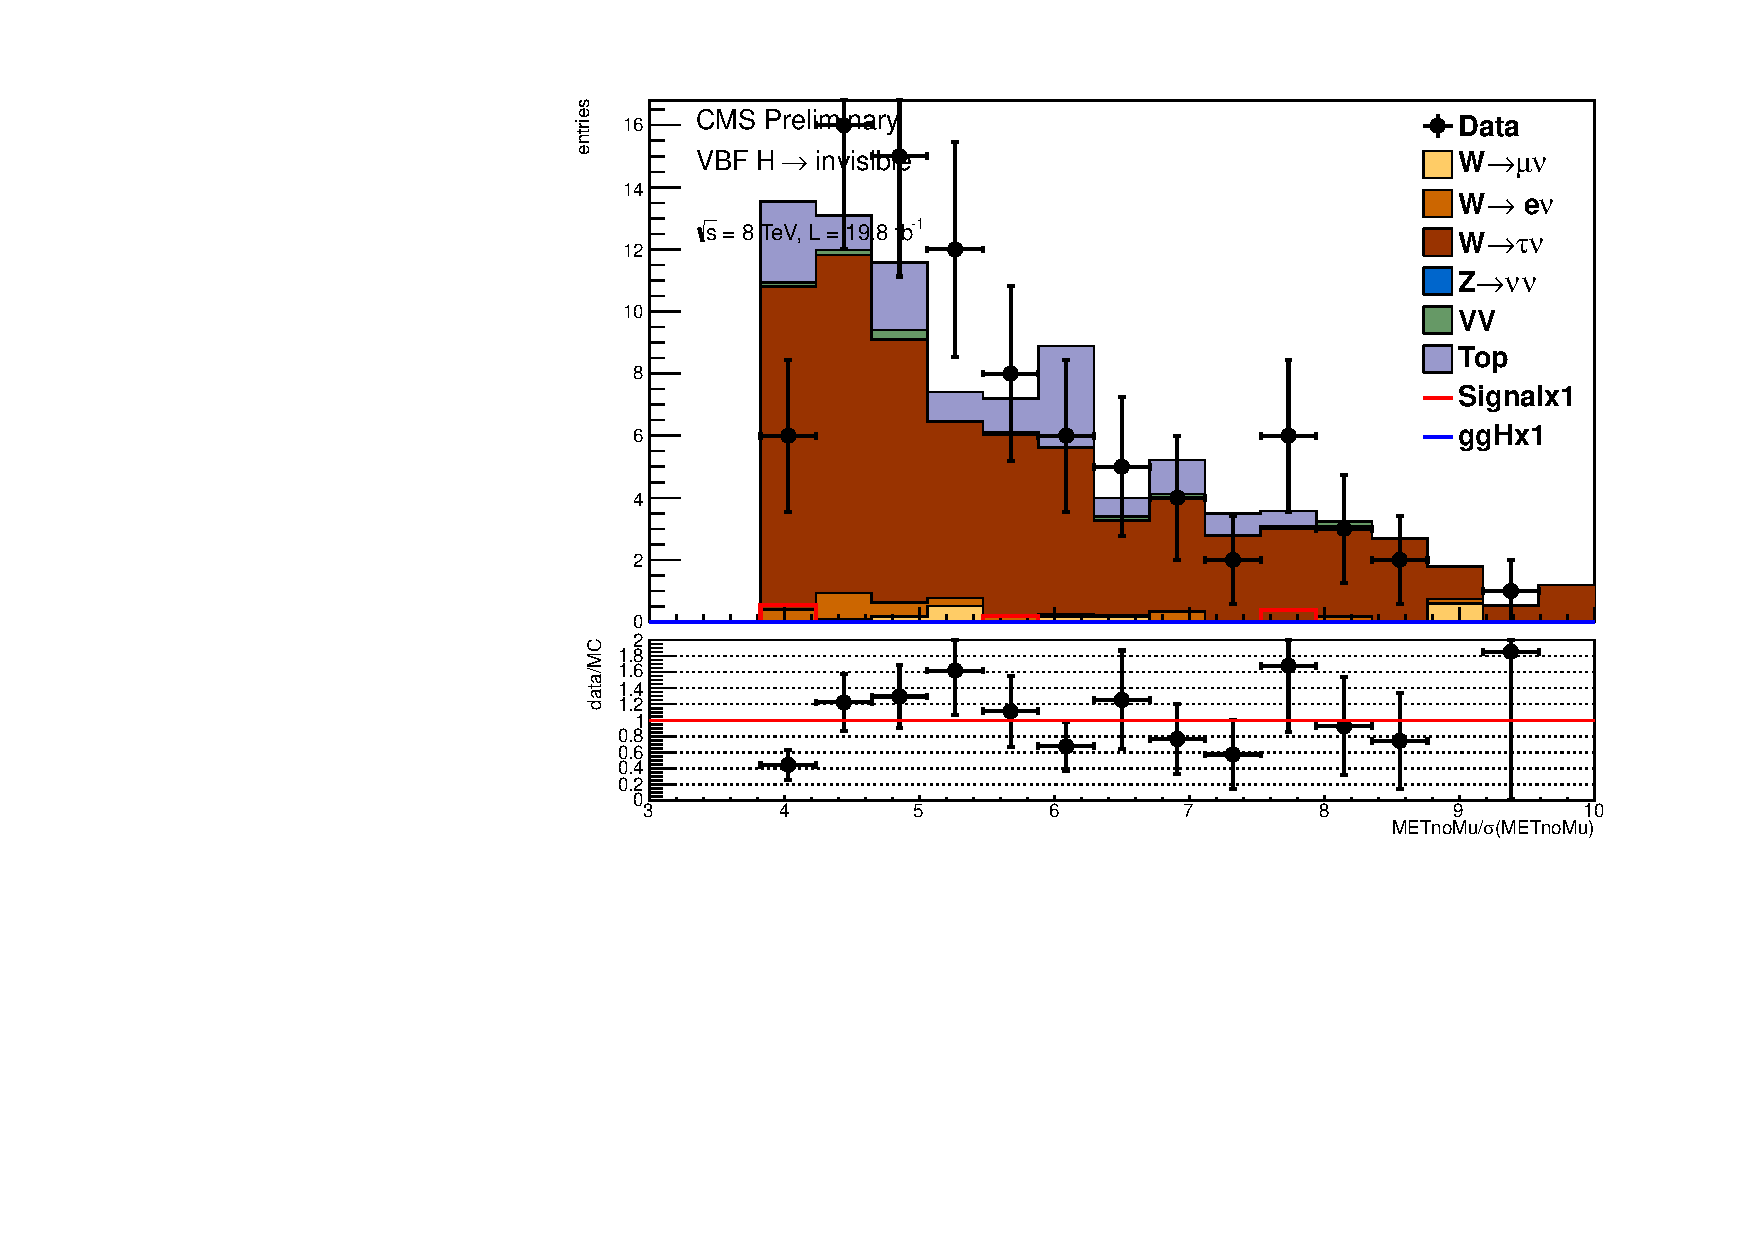
\includegraphics[clip=true,trim=0 0 0 360,width=\textwidth]{TalkPics/higgsexo031114/output_sigreg/taunu_metnomu_significance.pdf}

    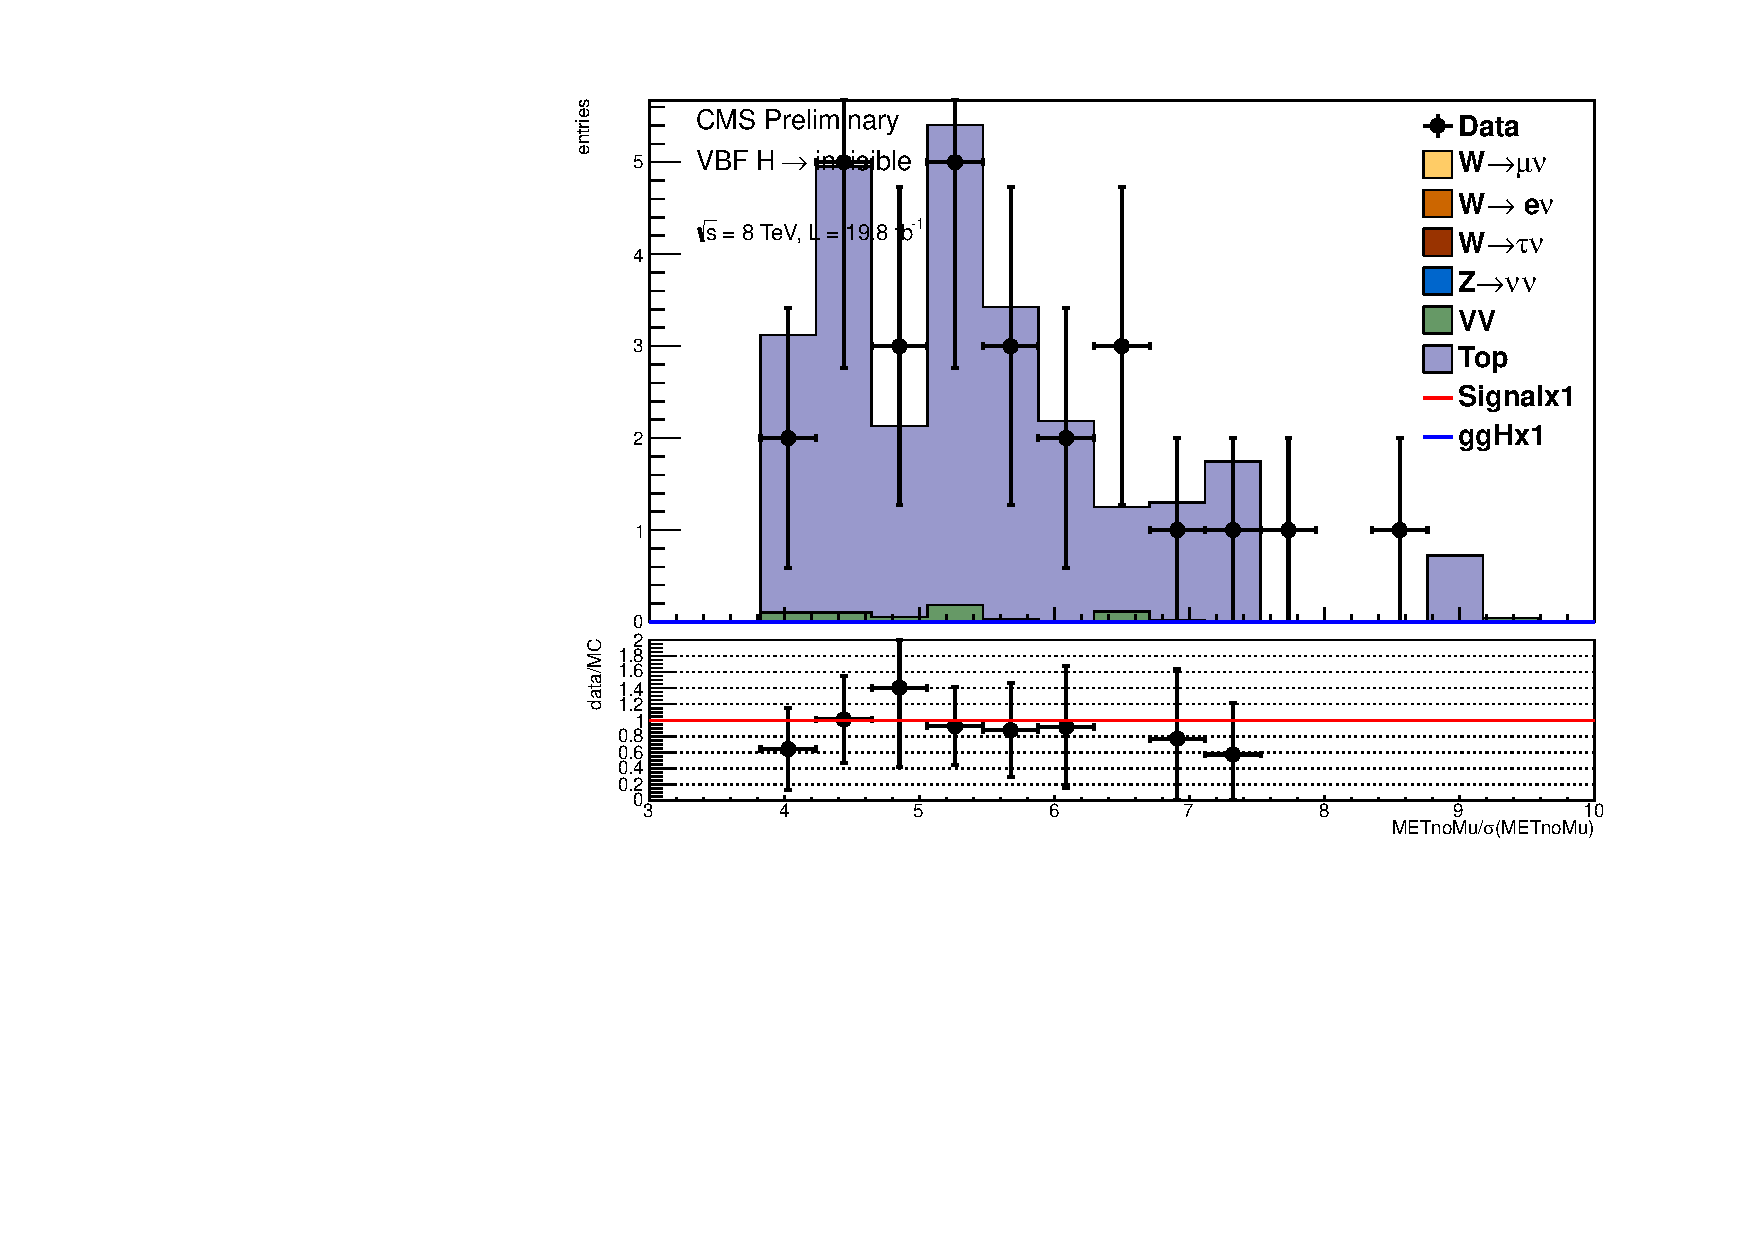
\includegraphics[width=\textwidth]{TalkPics/higgsexo031114/output_sigreg/top_metnomu_significance.pdf}
  \end{columns}
\end{frame}

\begin{frame}
  \frametitle{$W\rightarrow\tau\nu$ control region}
  \begin{columns}
    \column{.55\textwidth}
    \vspace{-.2cm}
    \begin{block}{}
      \scriptsize
      \begin{itemize}
      \item For other W+jets backgrounds control region is:
      \item[-] signal region with lepton veto replaced with a requirement for a single lepton
      \item For $W\rightarrow\tau\nu$ there are not enough events in this region: 2 events for $N_{C}^{Data}$
      \item[-] In prompt analysis we removed the central jet veto (CJV)
      \item CJV no longer used, so we remove the $\text{Min}\Delta\phi(all\,jets,\,METnomu)$ cut
      \item This leads to QCD contaminatin so we require:
      \item[-] $\text{Min}\Delta\phi(leading\,2\,jets,\,METnomu)>1.0$
      \item[-] We also add an $m_{T}>20$ GeV cut on the lepton-MET system to remove QCD contamination
      \end{itemize}
    \end{block}
    \column{.5\textwidth}
    \vspace{-.1cm}

    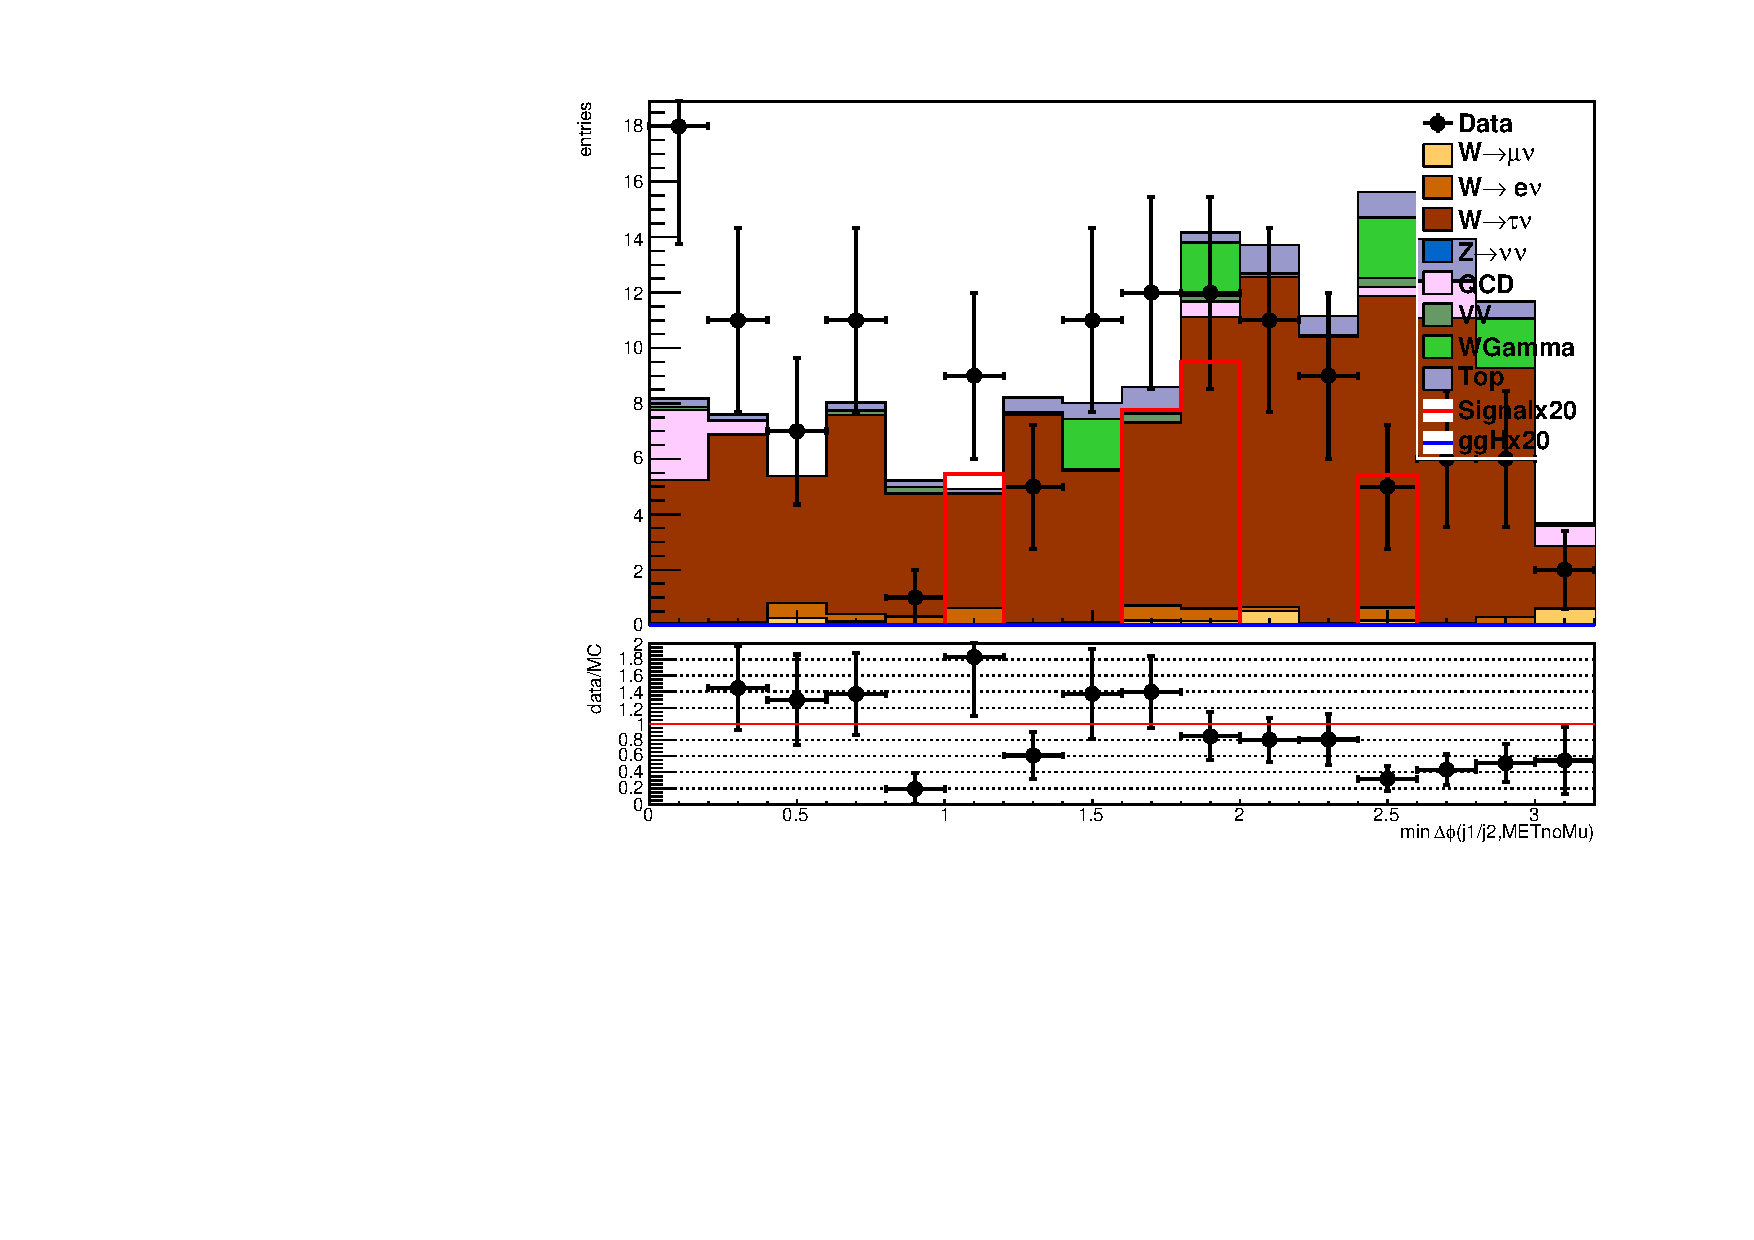
\includegraphics[clip=true,trim=0 0 0 20,width=.95\textwidth]{TalkPics/limits131014/leadingjetmetdphiforam.pdf}
    
    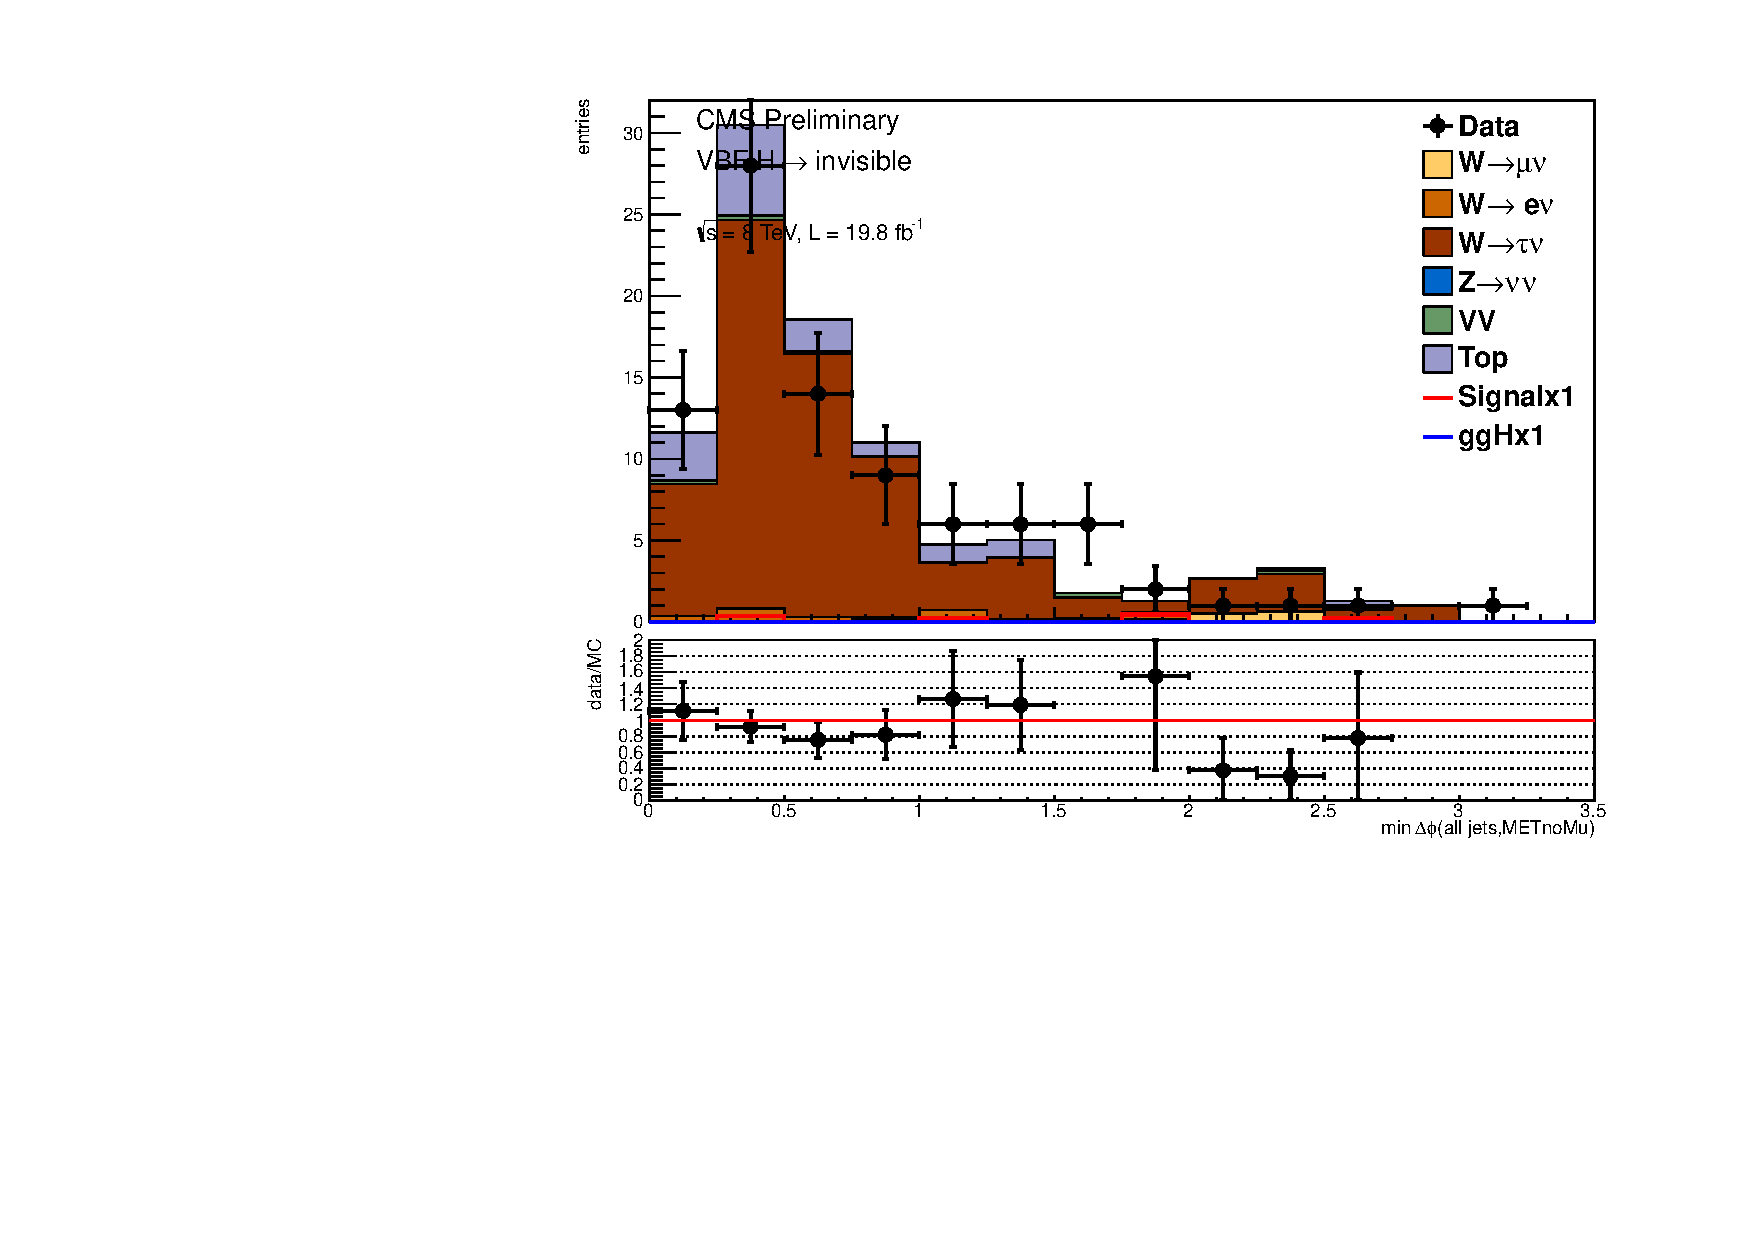
\includegraphics[clip=true,trim=0 0 0 20,width=.95\textwidth]{TalkPics/higgsexo031114/output_sigreg/taunu_alljetsmetnomu_mindphi.pdf}
  \end{columns}
\end{frame}

\begin{frame}
  \frametitle{$W\rightarrow\tau\nu$ control region}
  \begin{columns}
    \column{.55\textwidth}
    \begin{block}{}
      \scriptsize
      \begin{itemize}
      \item Estimate error from difference between control region and signal region cuts
      \item $W\rightarrow\mu\nu$ has enough events to see data driven weight variation with $\text{Min}\Delta\phi(all\,jets,\,METnomu)$ cut 
      \item[-] weight changes by 20\% when loosening cut from 2.5 to 1.0
      \item[-] We add a 20\% systematic on the $W\rightarrow\tau\nu$ background
      \end{itemize}
      \begin{tabular}{|l|c|c|}
        \hline
        $N_{C}^{data}$ & $88 \pm 9.4  (stat.)$\\
        $N_{C}^{bkg}$ & $15.2 \pm 4.8 (MC stat.)$  \\
        $N_{S}^{MC}$ & $176.1\pm 10.5  (MC stat.)$ \\
        $N_{C}^{MC}$ & $133.9 \pm 8.0 (MC stat.)$   \\
        \hline
        $N_{S}^{W}$ & \textcolor{red}{$95.7 \pm 12.3 (stat.) \pm 10.2 (MC stat.)$}  \\
        \hline
      \end{tabular}
    \end{block}
    \column{.5\textwidth}
    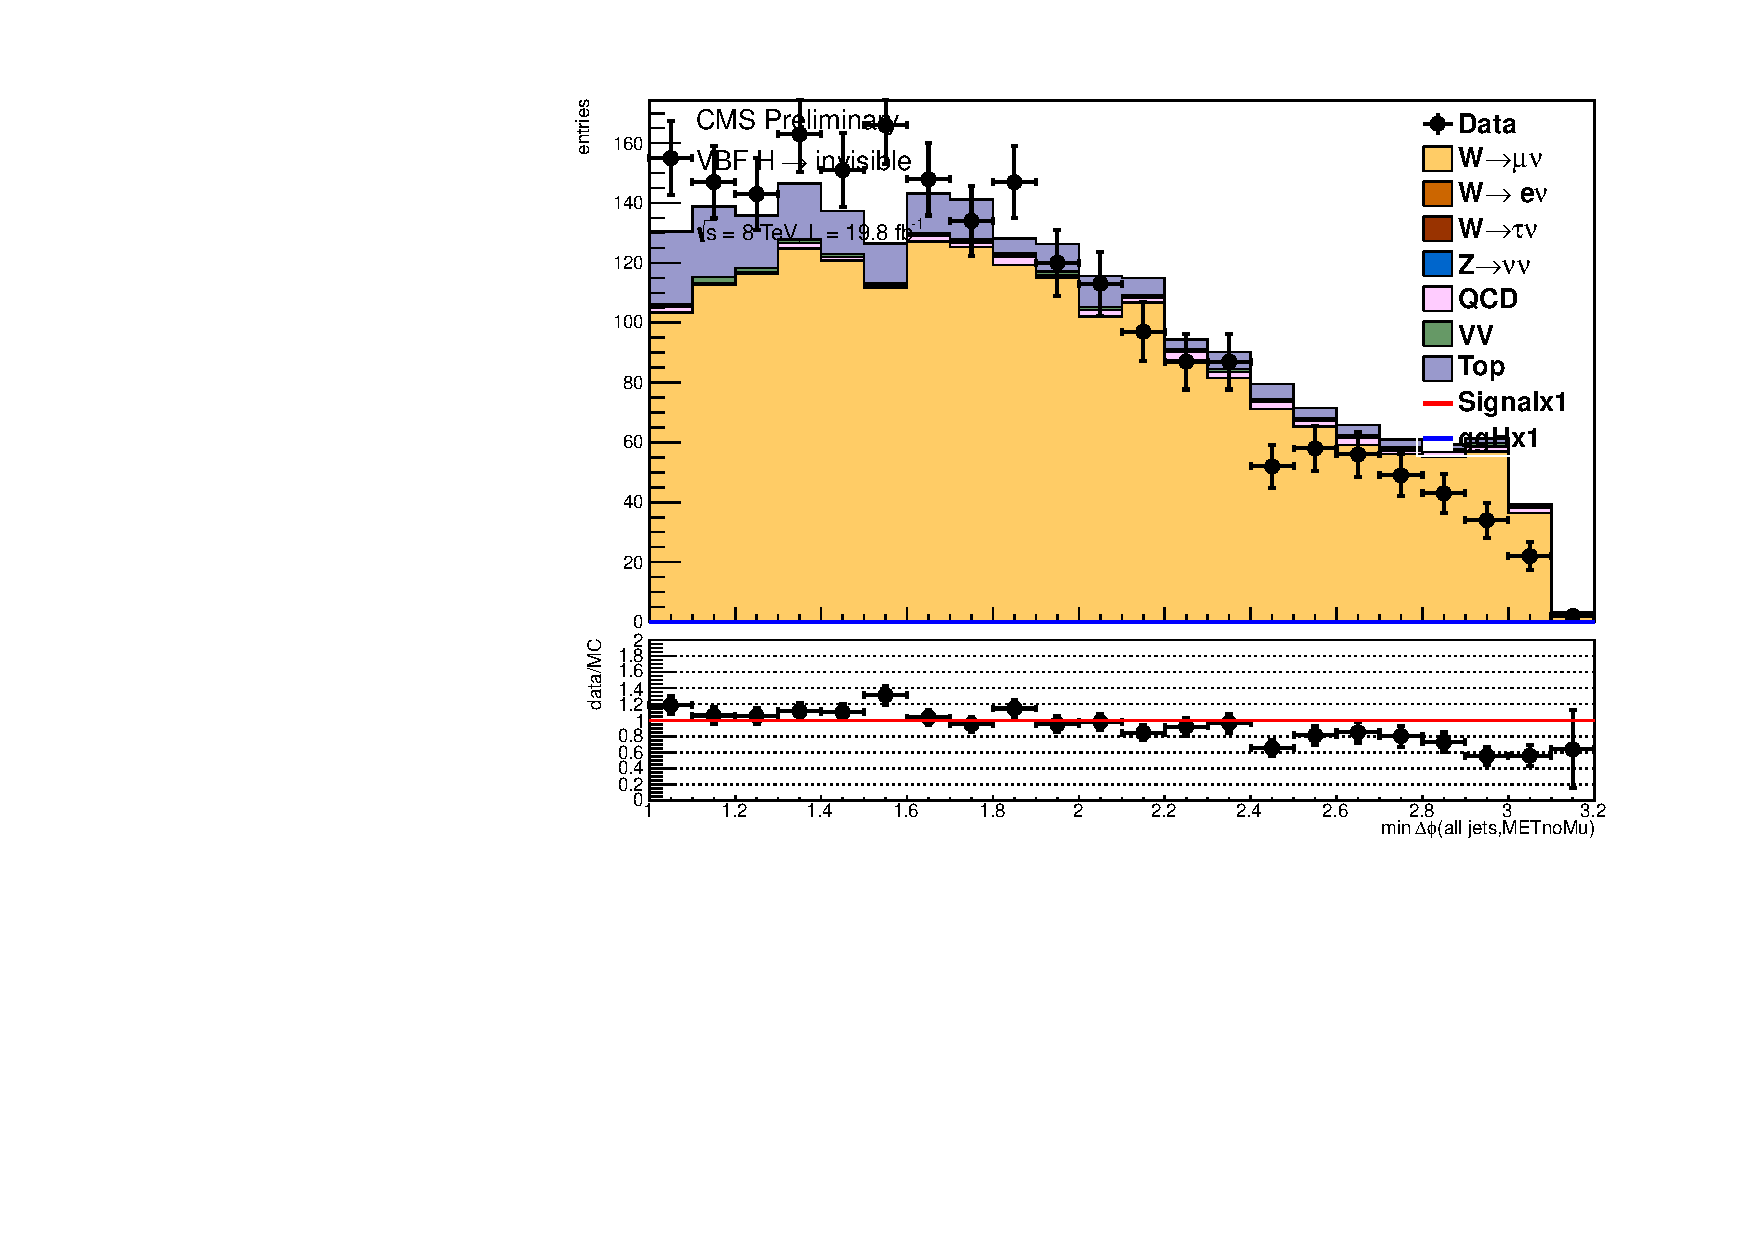
\includegraphics[clip=true,trim=0 0 0 20,width=.95\textwidth]{TalkPics/higgsexo031114/output_presel/munu_alljetsmetnomu_mindphi.pdf}

    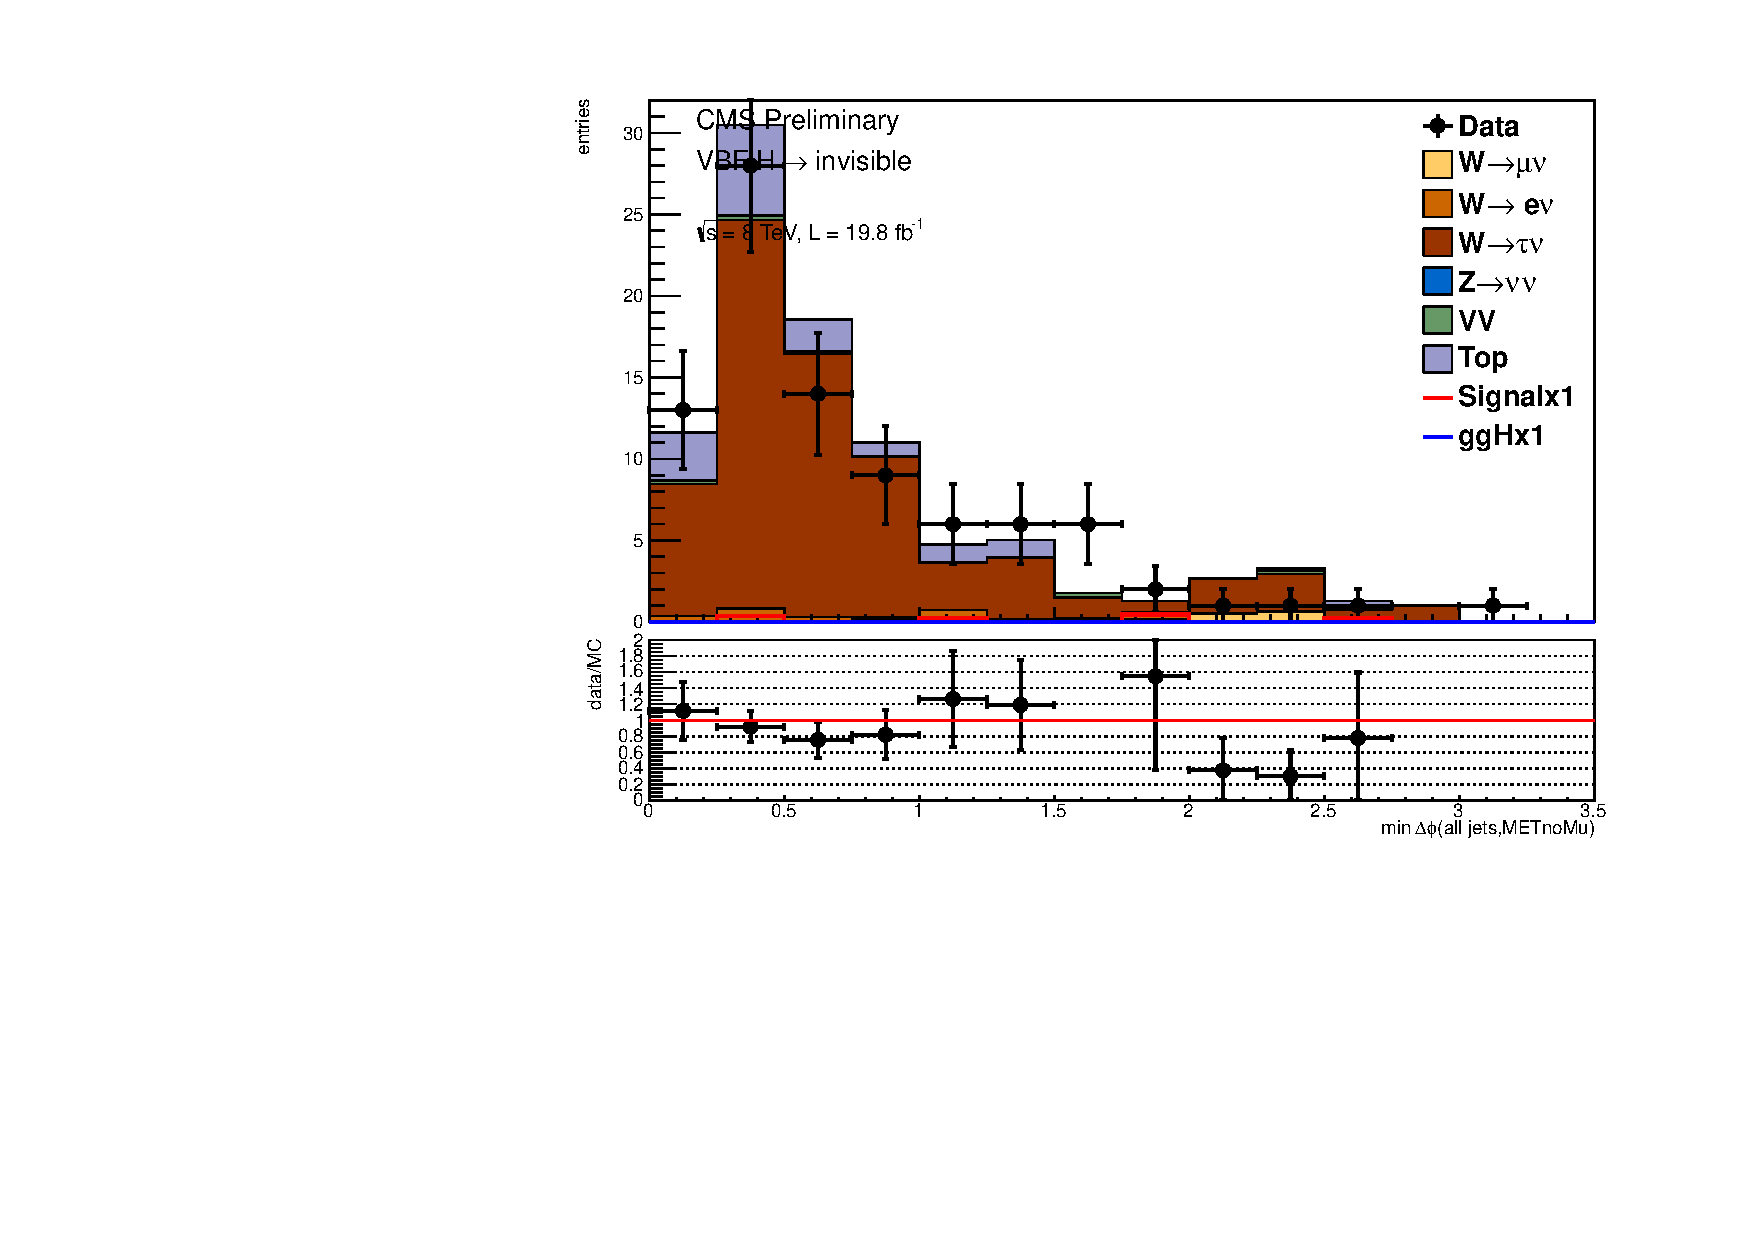
\includegraphics[clip=true,trim=0 0 0 20,width=.95\textwidth]{TalkPics/higgsexo031114/output_sigreg/taunu_alljetsmetnomu_mindphi.pdf}
  \end{columns}
\end{frame}


\begin{frame}
  \frametitle{QCD background estimation: Shape region choice}
   \begin{columns}
     \column{.55\textwidth}
     \begin{block}{}
       \scriptsize
       \begin{itemize}
       \item Try modelling QCD shape in preselection region 
       \item All QCD MC in region with low $\text{Min}\Delta\phi(all\,jets,\,METnomu)$
       \item Try inverted region with:
       \item[-] $\text{Min}\Delta\phi(all\,jets,\,METnomu)<1.0$
       \item[-] $\text{Min}\Delta\phi(leading\,jets,\,METnomu)>1.0$ 
       \item Has good shape agreement with enriched QCD MC
       \item Use shape taken from requiring:
       \item[-] $\text{Min}\Delta\phi(all\,jets,\,METnomu)<1.0$
       \item And replacing $\text{Min}\Delta\phi(all\,jets,\,METnomu)$ with $\text{Min}\Delta\phi(leading\,jets,\,METnomu)$
       \end{itemize}
     \end{block}
     \column{.5\textwidth}
     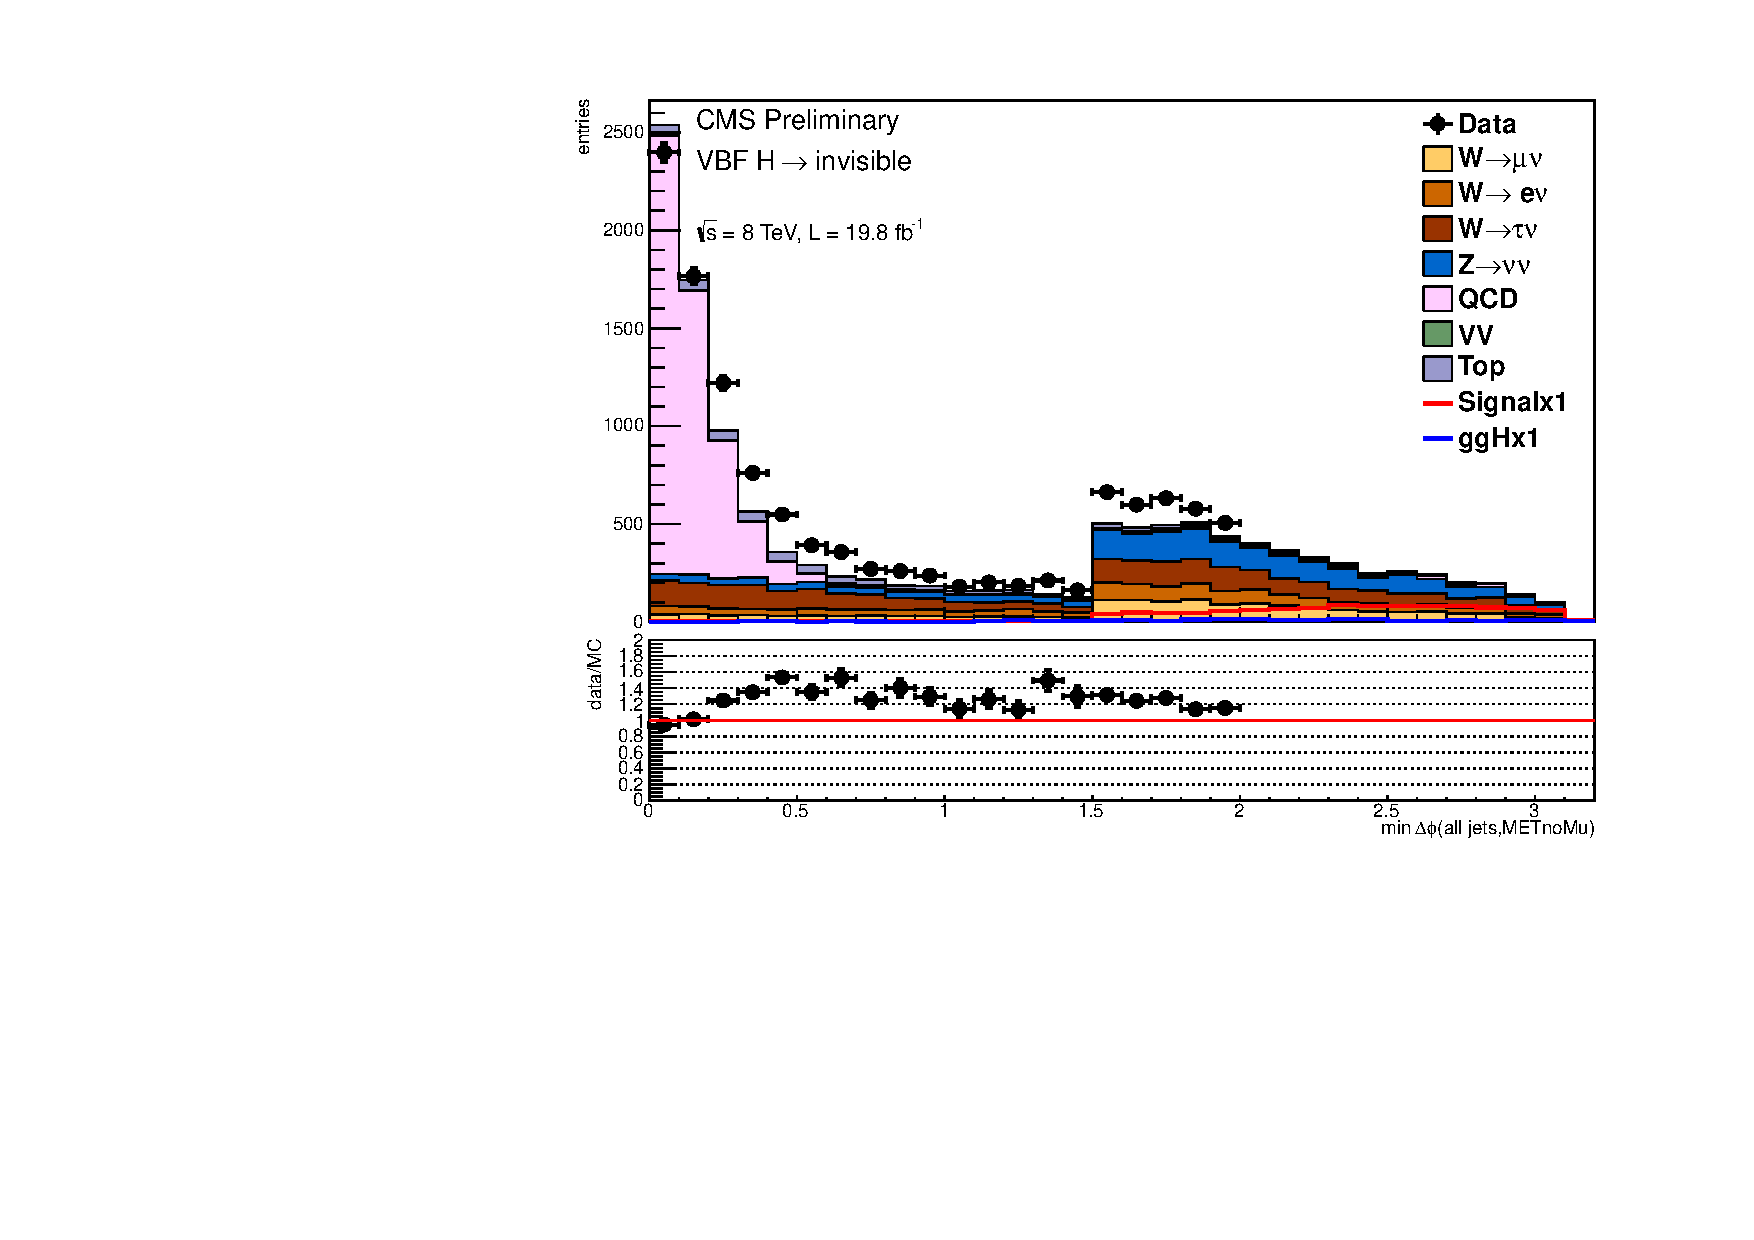
\includegraphics[clip=true,trim=0 0 0 20,width=.95\textwidth]{TalkPics/higgsexo031114/output_amqcd/nunu_alljetsmetnomu_mindphi.pdf}
     
     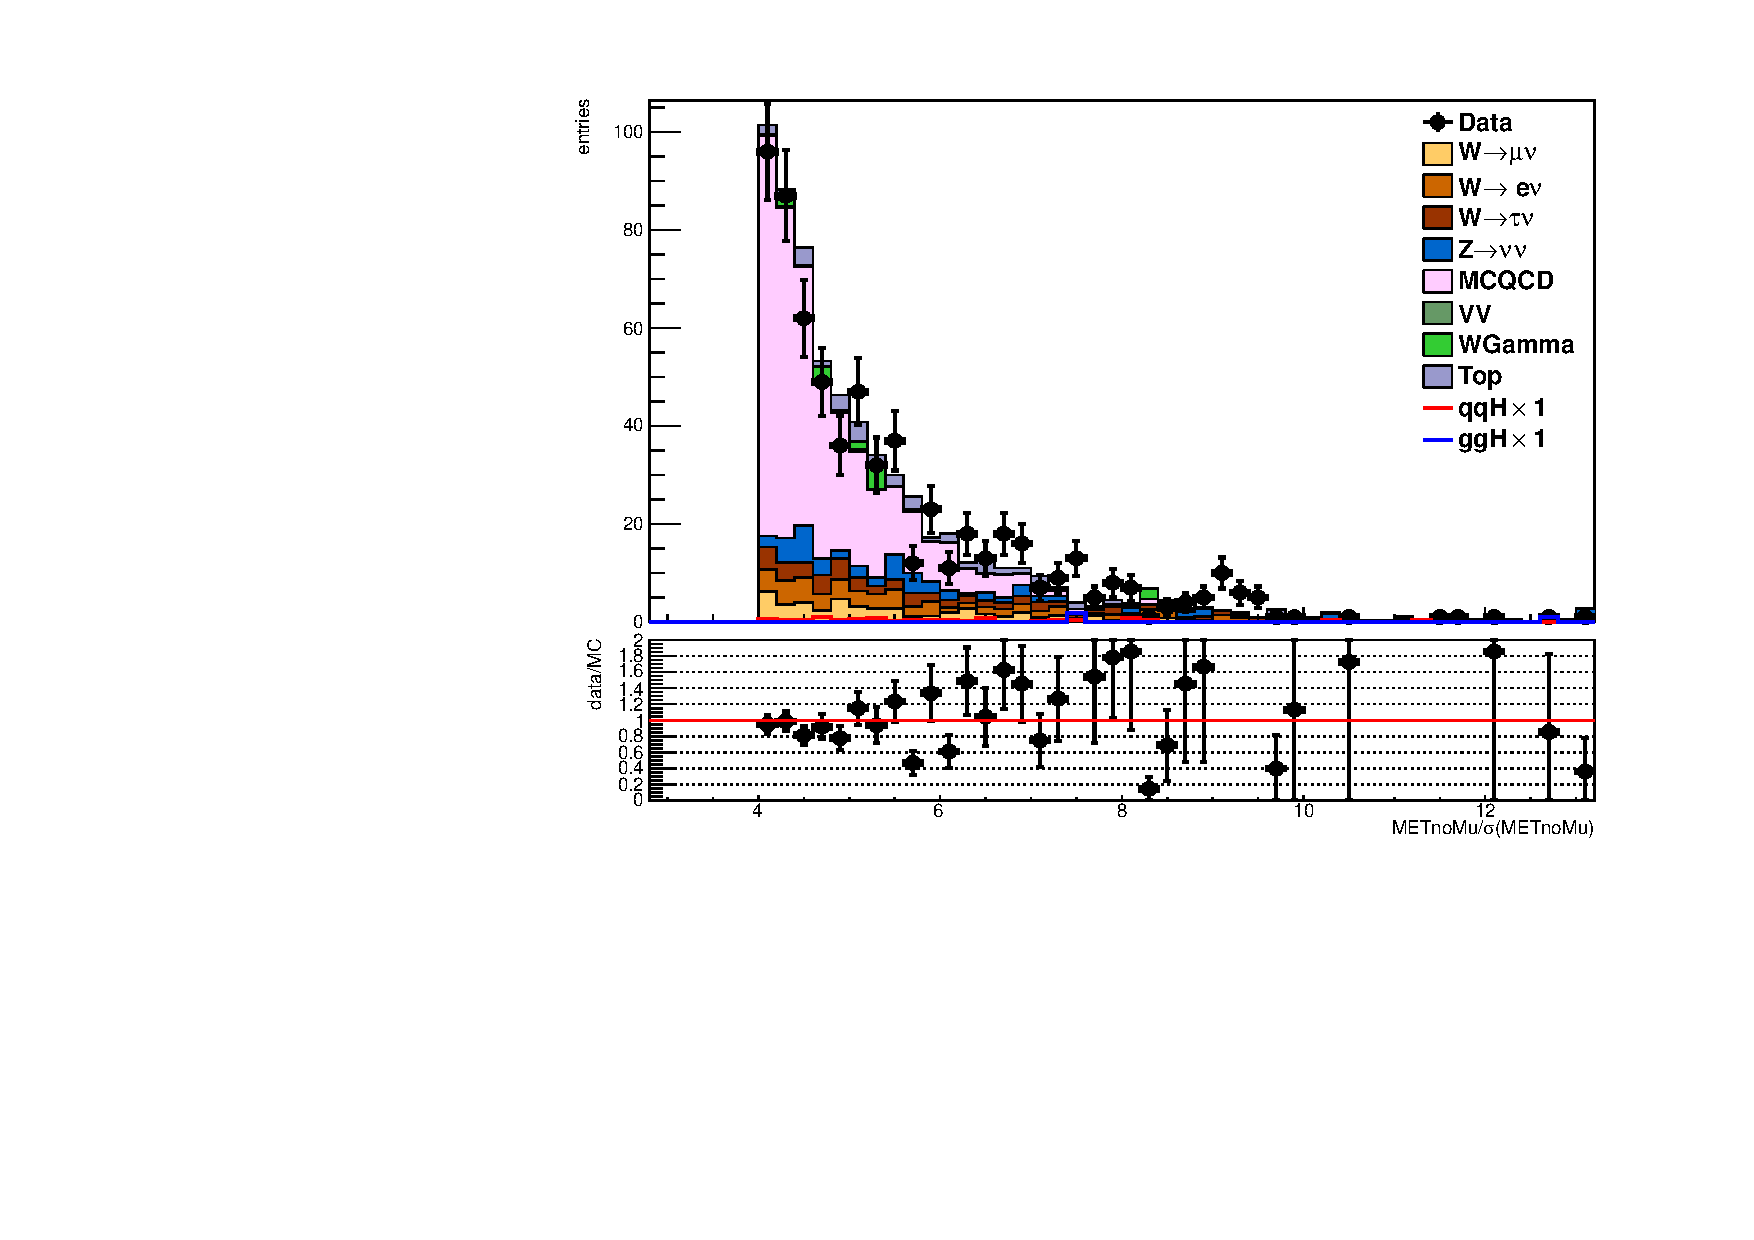
\includegraphics[clip=true,trim=0 0 0 20,width=.95\textwidth]{TalkPics/higgsexo031114/output_invqcd/qcd_metnomu_significance.pdf}
     
   \end{columns}
\end{frame}

\begin{frame}
  \frametitle{QCD background estimation: Scale factor}
   \begin{columns}
     \column{.55\textwidth}
      \begin{block}{}
        \scriptsize
        \begin{itemize}
        \item Unfortunately selection on $\text{Min}\Delta\phi(jets,METnomu)$ or $\frac{METnomu}{\sigma_{METnomu}}$ kills all QCD so cannot normalise
        \item Scale factor shows strong dependence on cut variables
        \item Norm 2 and 3 have large signal contamination
        \item[-] Norm 3 also has low stats and odd because requiring very significant met near a mismeasured object
        \item Fit scale factor variation in norm 1
        \item Check consistency in norm 2 and 3
        \end{itemize}
      \end{block}
     \column{.5\textwidth}
     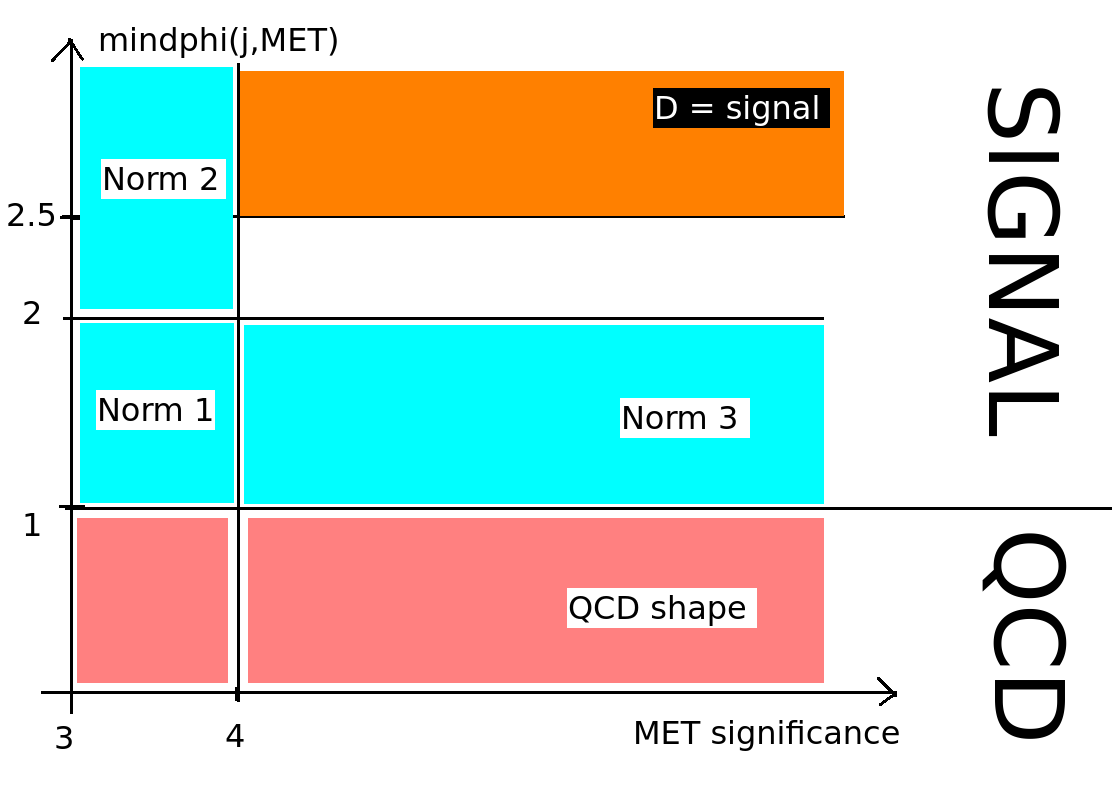
\includegraphics[clip=true,trim=0 0 0 20,width=.95\textwidth]{TalkPics/higgsexo031114/schema.png}  
   \end{columns}
\end{frame}

\begin{frame}
  \frametitle{Scale factor variation}
  \vspace{-.2cm}
  \scriptsize Norm 1

  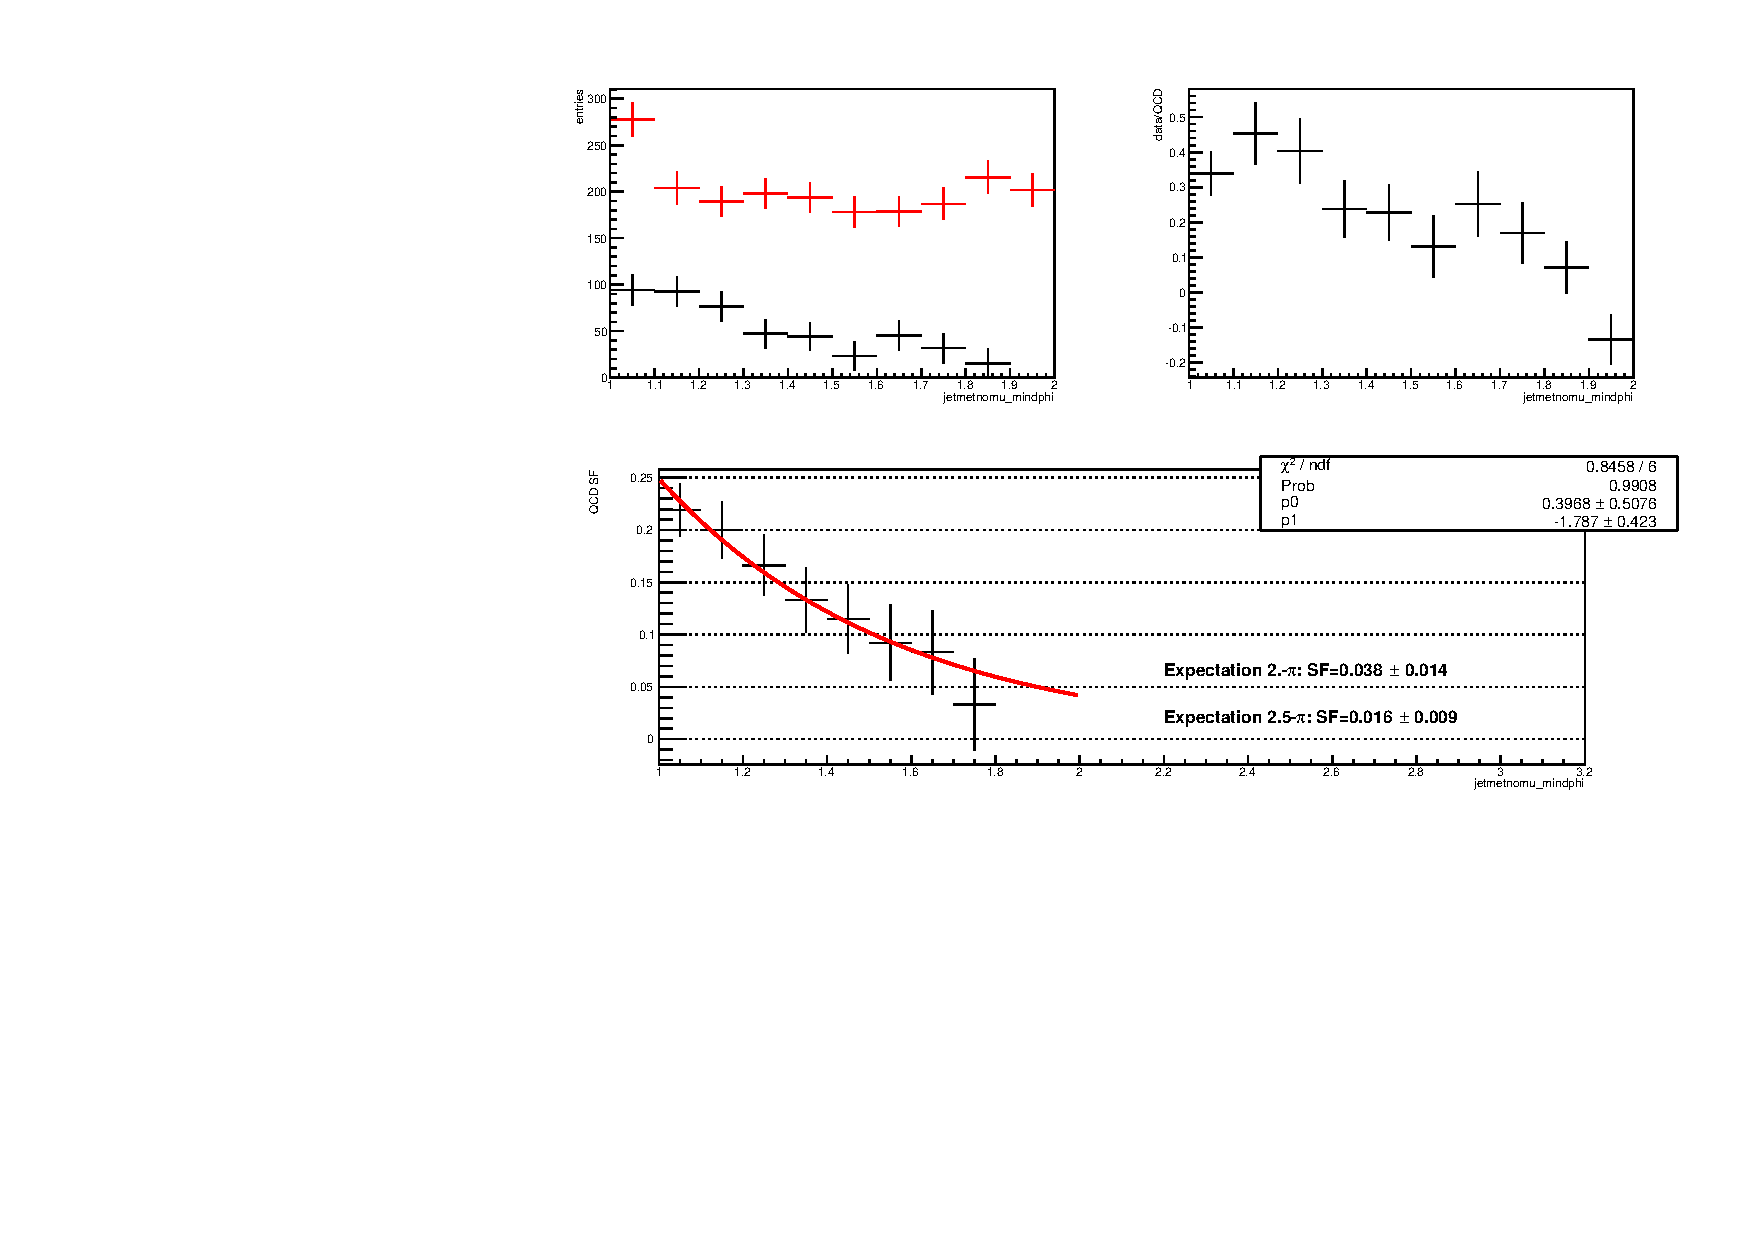
\includegraphics[clip=true,trim=0 0 0 180,width=.9\textwidth]{TalkPics/higgsexo031114/qcdEstimate/jetmetnomu_mindphi_norm1_SF.pdf}

  \vspace{-.2cm}

  \scriptsize Norm 1+2

  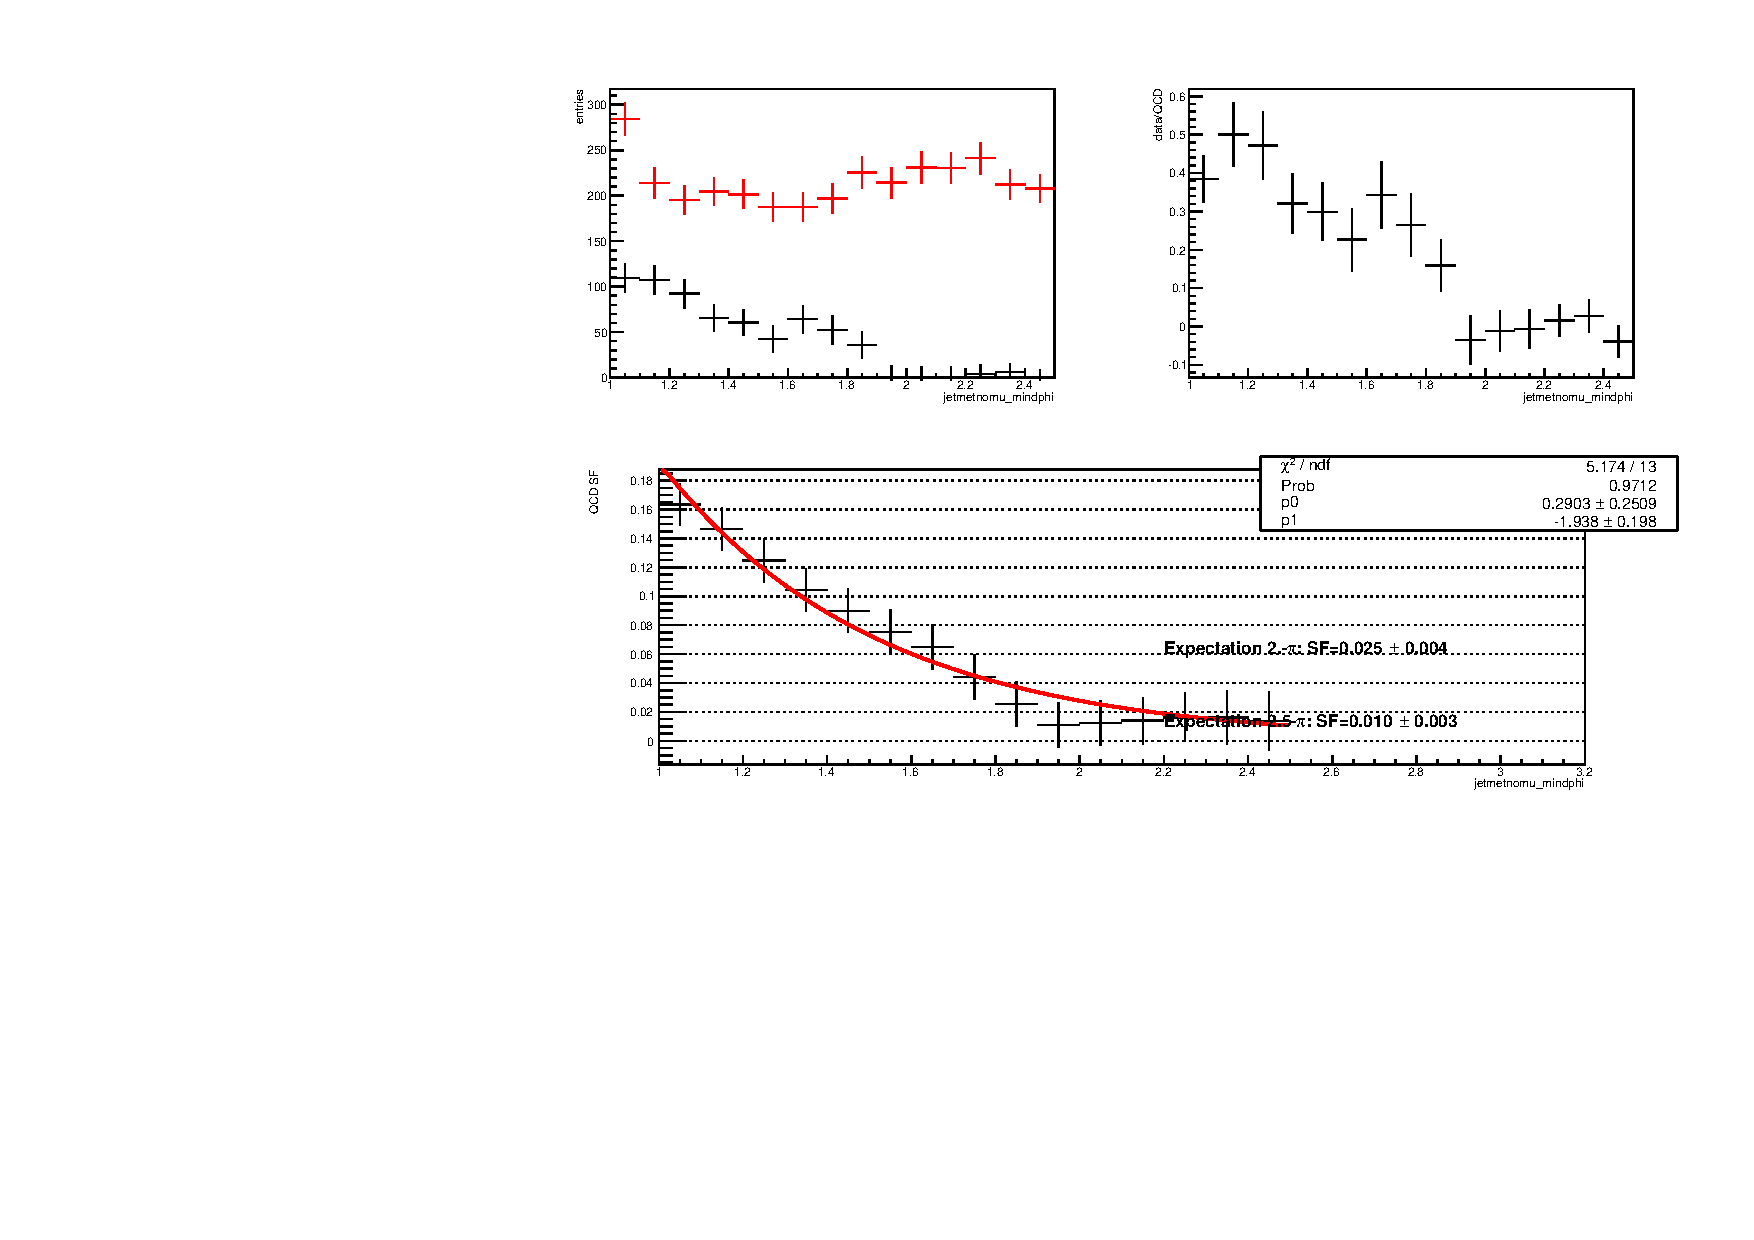
\includegraphics[clip=true,trim=0 0 0 180,width=.9\textwidth]{TalkPics/higgsexo031114/qcdEstimate/jetmetnomu_mindphi_norm12_SF.pdf}
\end{frame}

\begin{frame}
  \frametitle{QCD background estimation: Result and systematics}
  \begin{columns}
    \column{.75\textwidth}
     \begin{block}{}
       \centering
       \scriptsize
       \begin{tabular}{|l|c|c|c|}
         \hline
         Region & Factor & Extrapolation & Extrapolation \\
         & & mindphi$>2.5$ & metsig$>4$ \\
         \hline
         Norm 1 & 0.22 $\pm$ 0.03 & 0.016 $\pm$ 0.009 & 0.04 $\pm$ 0.03\\
         Norm 1+2 & 0.15 $\pm$ 0.02 & 0.010 $\pm$ 0.003 & 0.03 $\pm$ 0.02\\
         \rowcolor{yellow}Norm 1+3 & 0.41 $\pm$ 0.03 & 0.036 $\pm$ 0.062 & 1.10 $\pm$ 0.10\\
         Norm 2 & 0.08 $\pm$ 0.02 & - & 0.05$\pm$0.04 \\
         \rowcolor{yellow}Norm 3 & 1.22 $\pm$ 0.15 & 0.60$\pm$0.25 & - \\
         \hline
       \end{tabular}
     \end{block}
     \end{columns}
     \begin{block}{}
       \scriptsize
       \begin{itemize}
       \item Good agreement in all $\text{Min}\Delta\phi(all\,jets,\,METnomu)$ extrapolations
       \item Norm 3 agreement in metsig is poor
       \item[-] As norm 3 has low statistics and is an odd region: drop
       \item Use largest scale factor and largest relative error of remaining
       \item Final prediction: $N_{S}^{QCD}=17\pm 14$
       \item Expected limit 0.5\% better with no QCD, 0.5\% worse with double error
       \end{itemize}
     \end{block}
\end{frame}

\begin{frame}
  \frametitle{Results}
    \begin{columns}
      \column{.7\textwidth}
  \begin{block}{}
    \scriptsize
    \centering
    \begin{tabular}{|l|c|}
      \hline
      Process & Number of events \\
      \hline
      $Z\rightarrow\nu\nu$ & $141.9 \pm 36.4(\text{stat.}) \pm 15.0 (\text{MC stat.})$ \\
      $W\rightarrow e\nu$& $ 59.7\pm 7.7 (\text{stat.}) \pm 5.2 (\text{MC stat.})$ \\
      $W\rightarrow \mu\nu$& $81.2 \pm 5.6 (\text{stat.}) \pm 5.8 (\text{MC stat.})$ \\
      $W\rightarrow \tau\nu$& $95.7 \pm 12.3 (\text{stat.}) \pm 10.2 (\text{MC stat.})$ \\
      QCD & $ 17 \pm 14 $\\
      Top & $6.1\pm 1.2(\text{stat.}) \pm 1.4 (\text{MC stat.})$ \\
      VV & $ 6.0\pm  0.6(\text{MC stat.})$ \\
      \hline
      Total bkg. & {\color{red}$404 \pm 39.6 (\text{stat.}) \pm 19.8 (\text{MC stat.})$} \\
      \hline
      VBF signal & $313.5 \pm 9.4 (\text{MC stat.})$ \\
      ggH signal & $22.5 \pm  6.0 (\text{MC stat.})$ \\
      \hline
      Total signal & {\color{red}$ 336 \pm 11.1 (\text{MC stat.})$} \\
      \hline
    \end{tabular}
  \end{block}
    \end{columns}
\end{frame}

\begin{frame}
  \frametitle{Expected limits}
   \begin{columns}
     \column{.55\textwidth}
     \begin{block}{}
       \scriptsize
       \begin{itemize}
       \item Used Higgs combine package with Asymptotic CLs method
       \item Performed a single bin counting experiment
       \item Analysis blind so have expected limits only
       \item 95\% C.L. Median limit on B(H$\rightarrow$inv.) for $m_{H}=125$ GeV is: {\color{red}31\%}
       \item[-] 1$\sigma$ band is 23-43\%
       \item[-] 2$\sigma$ band is 17-57\%
       \item Prompt analysis expected limit was 49\%
       \item We intend to run other mass points:
       \item 110, 150, 200, 300 and 400 GeV
       \end{itemize}
     \end{block}
     \column{.5\textwidth}
     \begin{block}{}
       \scriptsize
       \centering
       \begin{tabular}{|c|}
         \hline
         Uncertainties by decreasing impact \\
         \hline
         Control region statistics \\
         $Z\rightarrow\nu\nu$-$Z/\gamma^{*}\rightarrow\mu\mu$ extrapolation\\ JES \\
         $W\rightarrow\tau\nu$ extrapolation \\MC statistics \\
         QCD systematics\\ lepton ID efficiency \\
         JER\\ UES\\ luminosity\\ PU weighting \\
         theory uncertainties \\
         \hline
       \end{tabular}
     \end{block}
   \end{columns}
\end{frame}

%!!BDT FIRST LOOK  WITH CAVEATS
\begin{frame}
  \frametitle{BDT Study}
  \begin{columns}
    \column{.55\textwidth}
    \begin{block}{}
      \scriptsize
      \begin{itemize}
      \item Had a quick look at MVA analysis
      \item Started from cut based signal region
      \item[-] Only region with negligible QCD
      \item Best expected limit obtained 30\%
      \item[-] Does not take into account any increased systematic
      \item[-] Therefore unlikely to be worthwhile
      \item New variables could make MVA worthwile
      \item Ability to model QCD would enable looser starting selection which may make MVA worthwhile
      \end{itemize}
    \end{block}
    \column{.5\textwidth}
    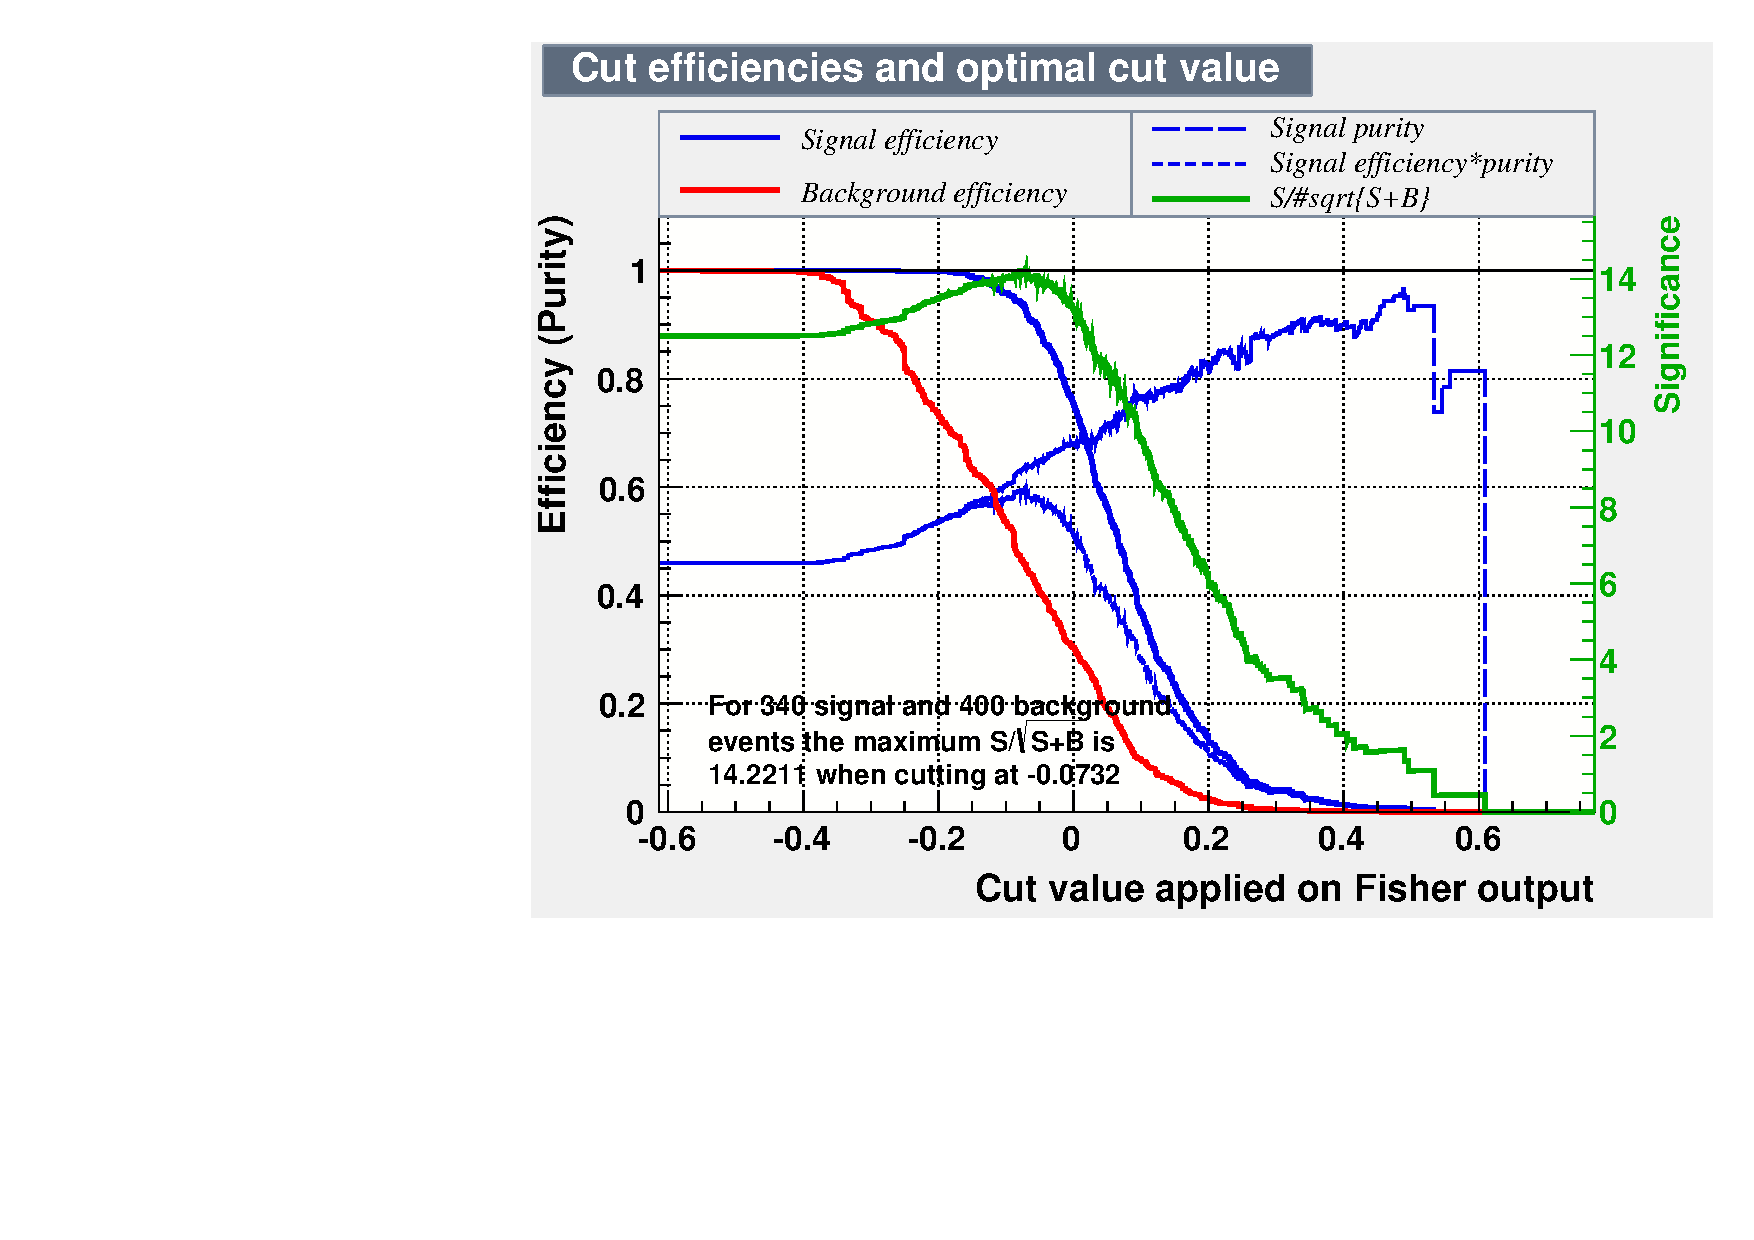
\includegraphics[width=\textwidth]{TalkPics/higgsexo031114/fishersoverb.pdf}
  \end{columns}
\end{frame}

\begin{frame}
  \frametitle{Summary}
  \label{lastframe}
  \begin{block}{}
    \begin{itemize}
    \item QCD modelling investigated
    \item[-] No adequate shape model found
    \item Cut based analysis designed to make QCD negligible
    \item[-] Can then accept remaining QCD estimate with large error
    \item MVA investigated
    \item[-] Not sufficient benefit without new variables or looser preselection
    \item Full cut based analysis presented
    \item[-] Expected limit {\color{red}31\%}
    \item[-] Improved from 49\% for prompt analysis
    \end{itemize}
  \end{block}
  %!!WOULD NEED CONTROL TRIGGERS ETC.
\end{frame}

\begin{frame}
  \frametitle{Backup}
\end{frame}

%!!POPULATE
%!!DETAILS OF QCD STUDIES
%!!MORE BDT INFO
\begin{frame}{VBF enriched QCD MC}
  \vspace{-.3cm}

  \begin{columns}
    \column{0.45\linewidth} 
    \begin{block}{\begin{tiny}MC Filter: Vectorial sum of neutrino $E_T$\end{tiny}}
      \begin{itemize}
      \item $\sum E_\perp(\vec{\nu}) > 40$ $GeV$
      \end{itemize}
    \end{block}
    \vspace{-.3cm}
    \begin{block}{\begin{tiny}MC Filter: Dijet Filter\end{tiny}}
      \tiny
      \begin{itemize}
      \item Select jets with:
        \begin{itemize}
          \scriptsize
        \item $p_\perp>20$ $GeV$
        \item $|\eta|<5.0$
        \end{itemize}
      \item From selected jets at least one pair with:
        \begin{itemize}
          \scriptsize
        \item $m_{jj}>700$ $GeV$
        \item $\Delta\eta>3.2$
        \end{itemize}  
      \end{itemize}
    \end{block}
    \column{0.45\linewidth} 
    \begin{block}{\tiny QCD Inc 80-600 $GeV$}
      \tiny
      \centering
      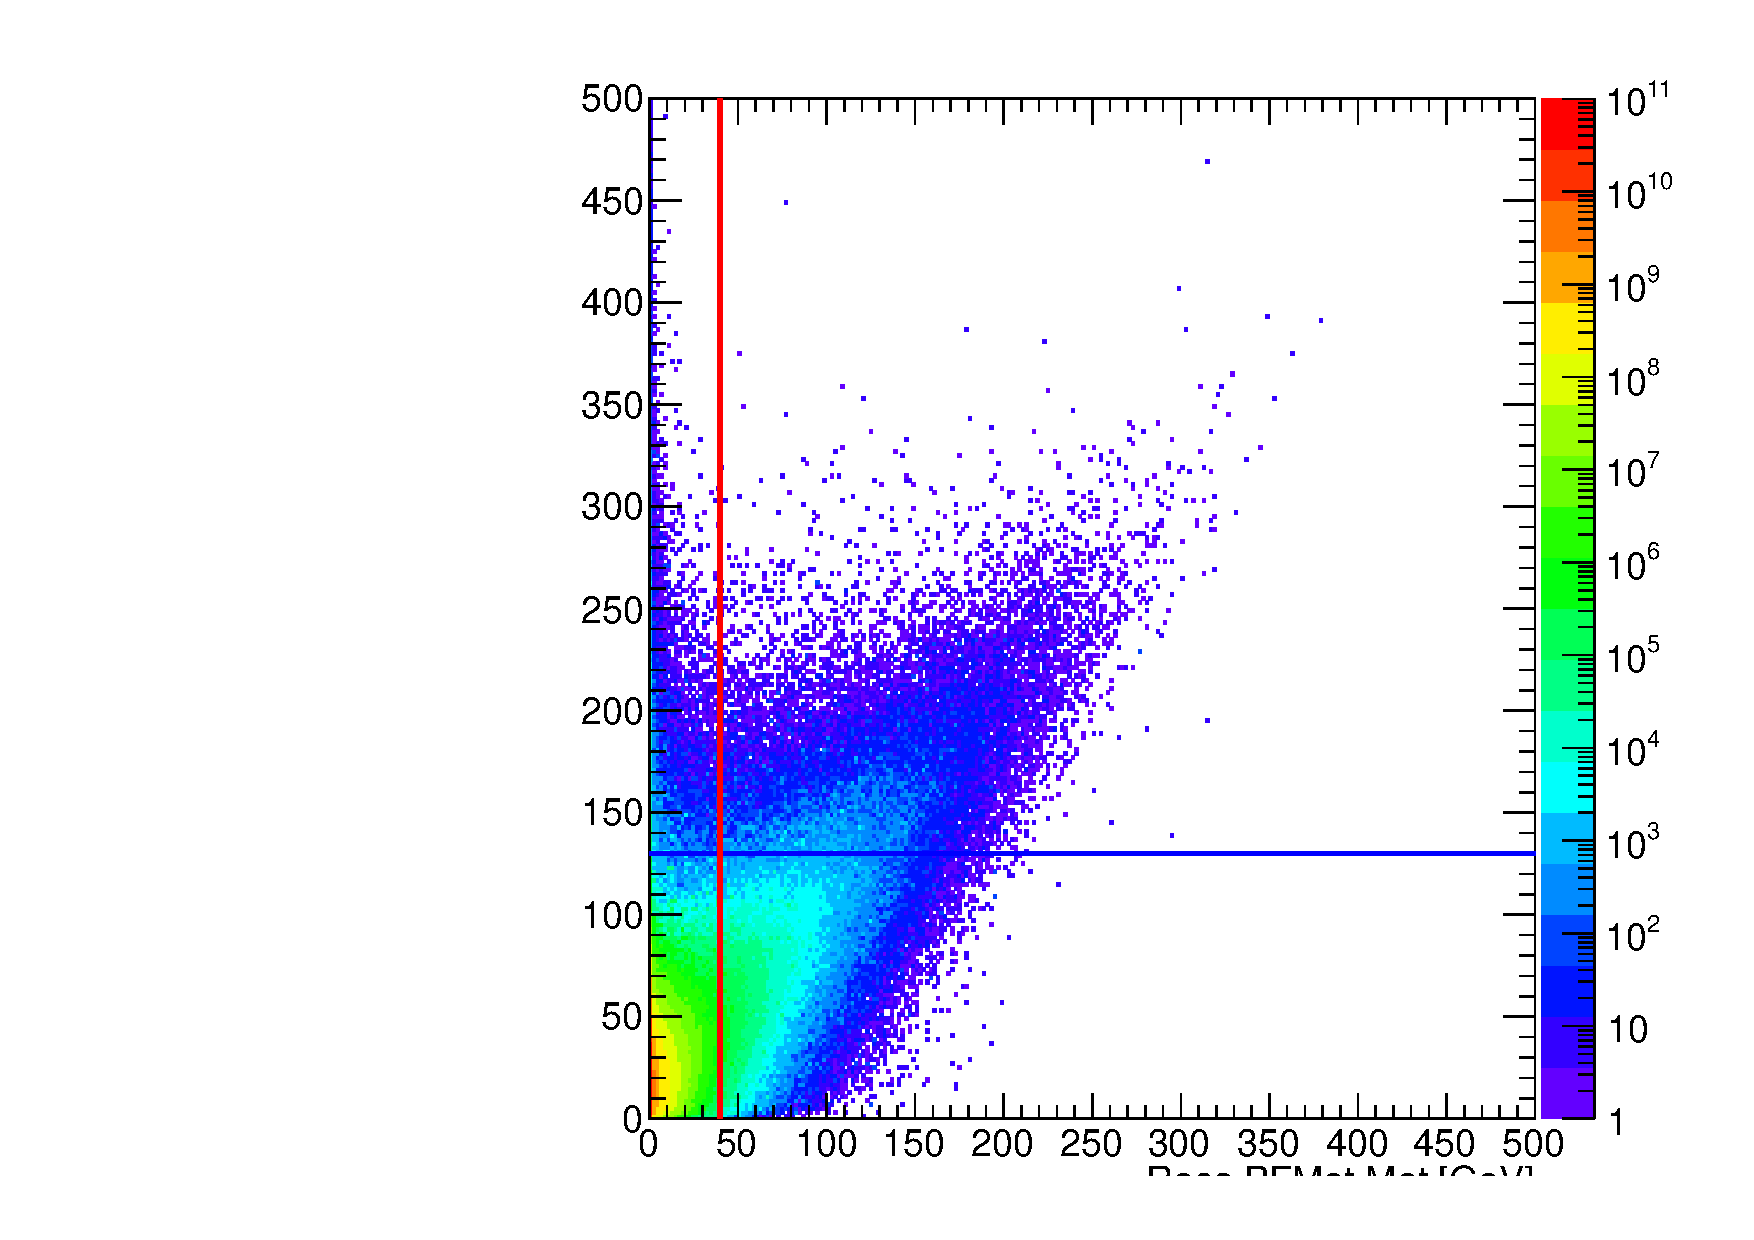
\includegraphics[width=0.7\linewidth]{TalkPics/higgsexo031114/MC_QCDIncAll_GenVsReco_met}

      There 2 distict populations of events: real and fake met.
    \end{block}
\end{columns}
  \vspace{-.1cm}

\begin{block}
  \scriptsize
  \centering
  \resizebox{0.8\linewidth}{!}{
    \begin{tabular}{|c|r|c|r|c|c|}
      \hline
      Sample          &       Ev. Gen. & Filter Eff. &  Events &  XS $[pb]$ & Eq. Lumi. $[fb^{-1}]$ \\
      \hline \hline
      QCD-Pt-80to120  & 39376000000 &    0.000049 & 1614416 &  1033680 &  38.09 \\
      QCD-Pt-120to170 &  7000000000 &    0.000283 & 2051000 & 156293.3 &  44.79 \\
      QCD-Pt-170to300 &  1375000000 &    0.000987 & 1391500 & 34138.15 &  40.28 \\
      QCD-Pt-300to470 &    80000000 &    0.002659 &  207840 & 1759.549 &  45.47 \\
      QCD-Pt-470to600 &    25000000 &    0.004127 &  104675 & 113.8791 & 219.53 \\
      \hline
    \end{tabular}
  }
\end{block}

\end{frame}

\begin{frame}
  \frametitle{QCD Data-Driven: j1j3, j2j3 shape}
  \centering
    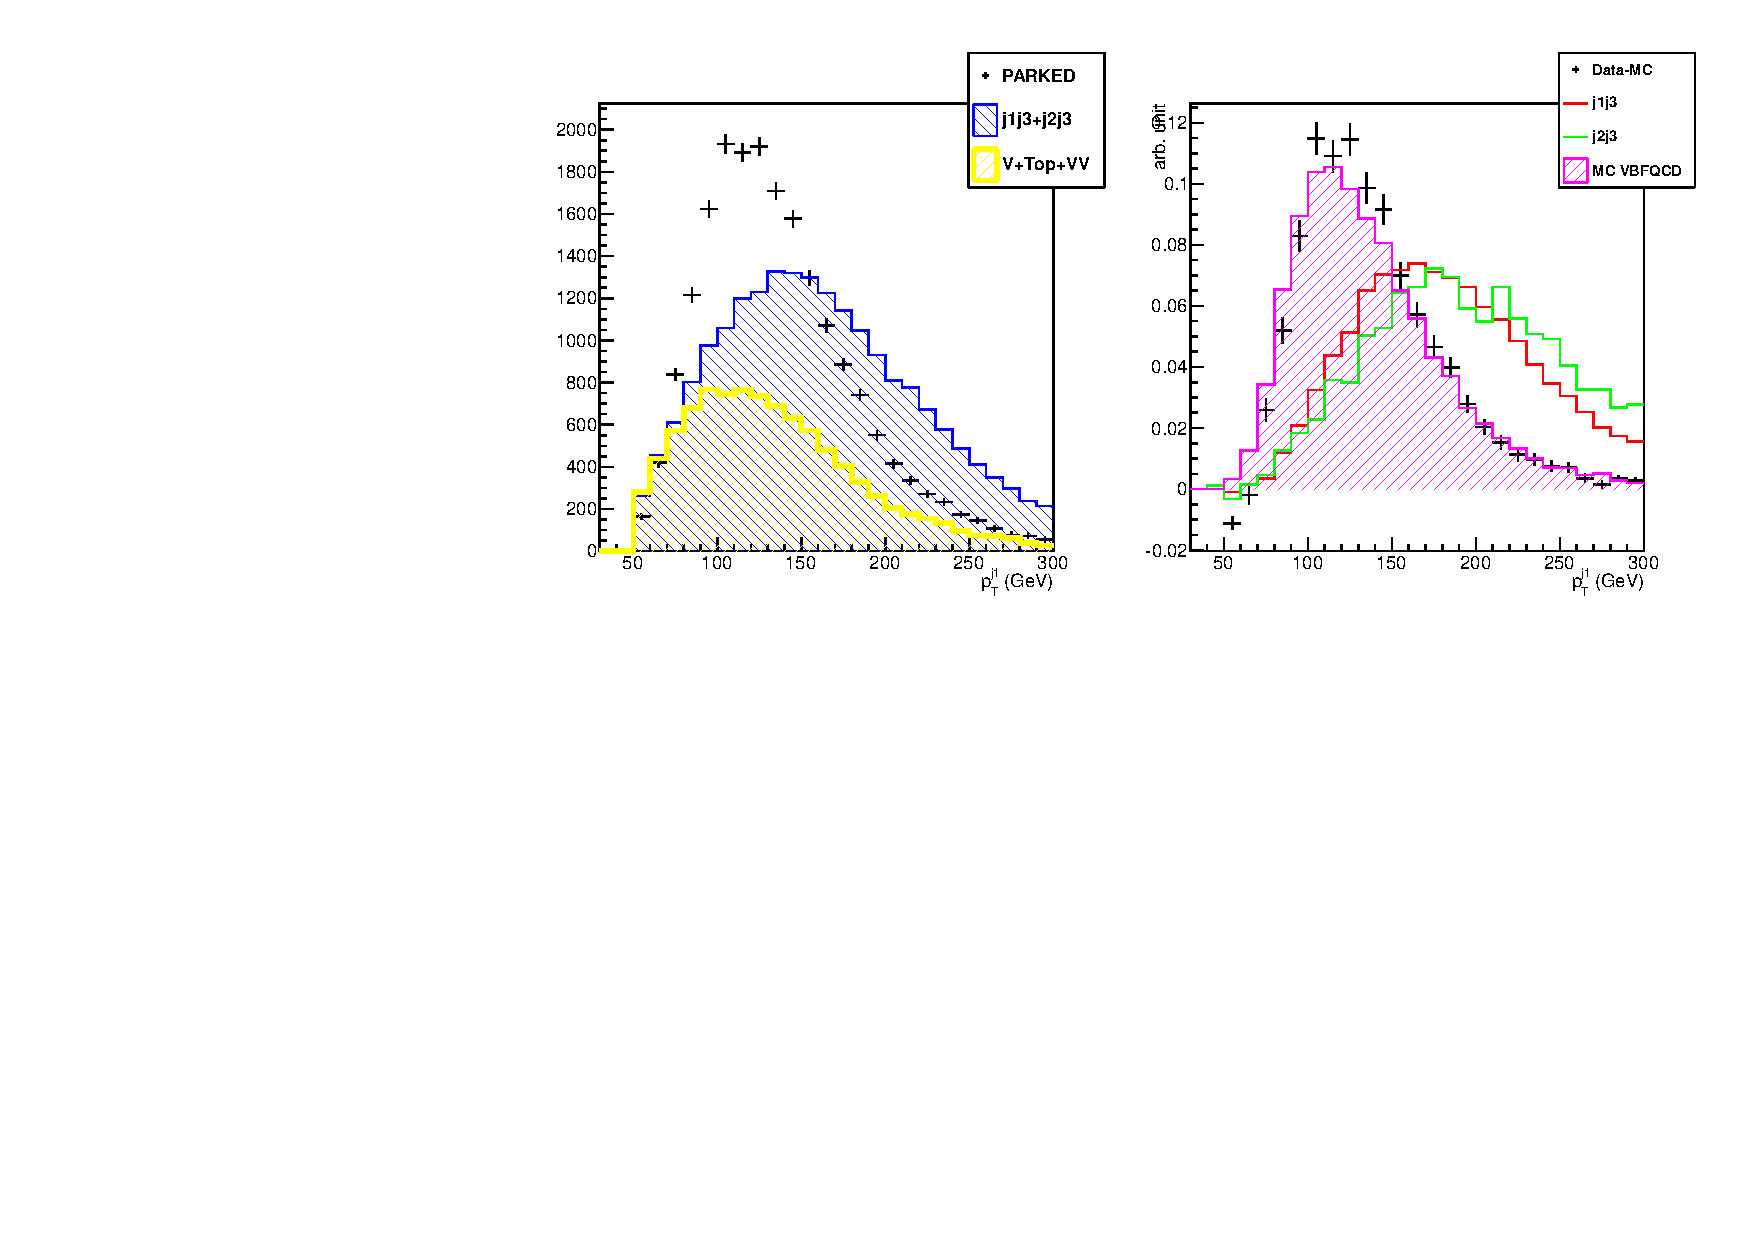
\includegraphics[width=.42\textwidth]{TalkPics/higgsexo031114/output_qcdJiJj/DataMC_PARKED_jet1_pt.pdf}
    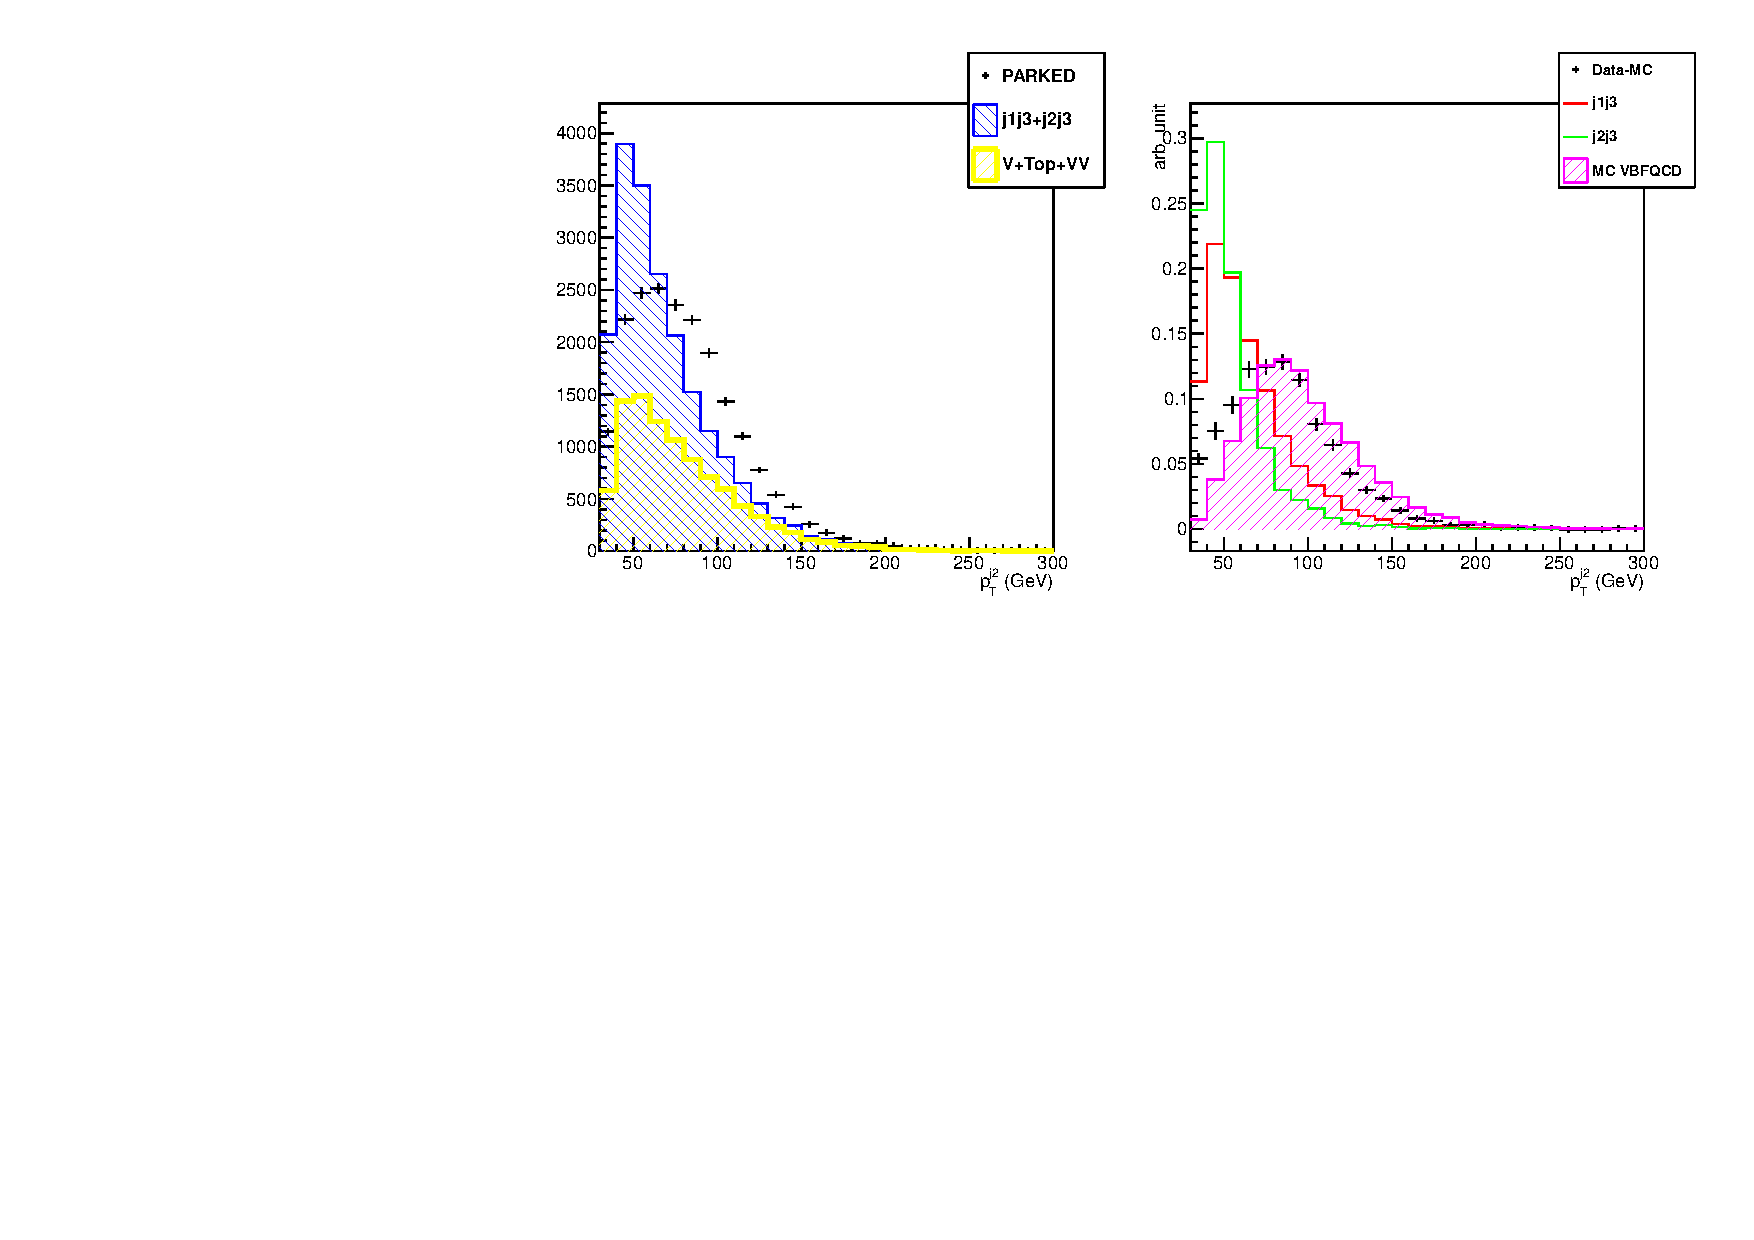
\includegraphics[width=.42\textwidth]{TalkPics/higgsexo031114/output_qcdJiJj/DataMC_PARKED_jet2_pt.pdf}

    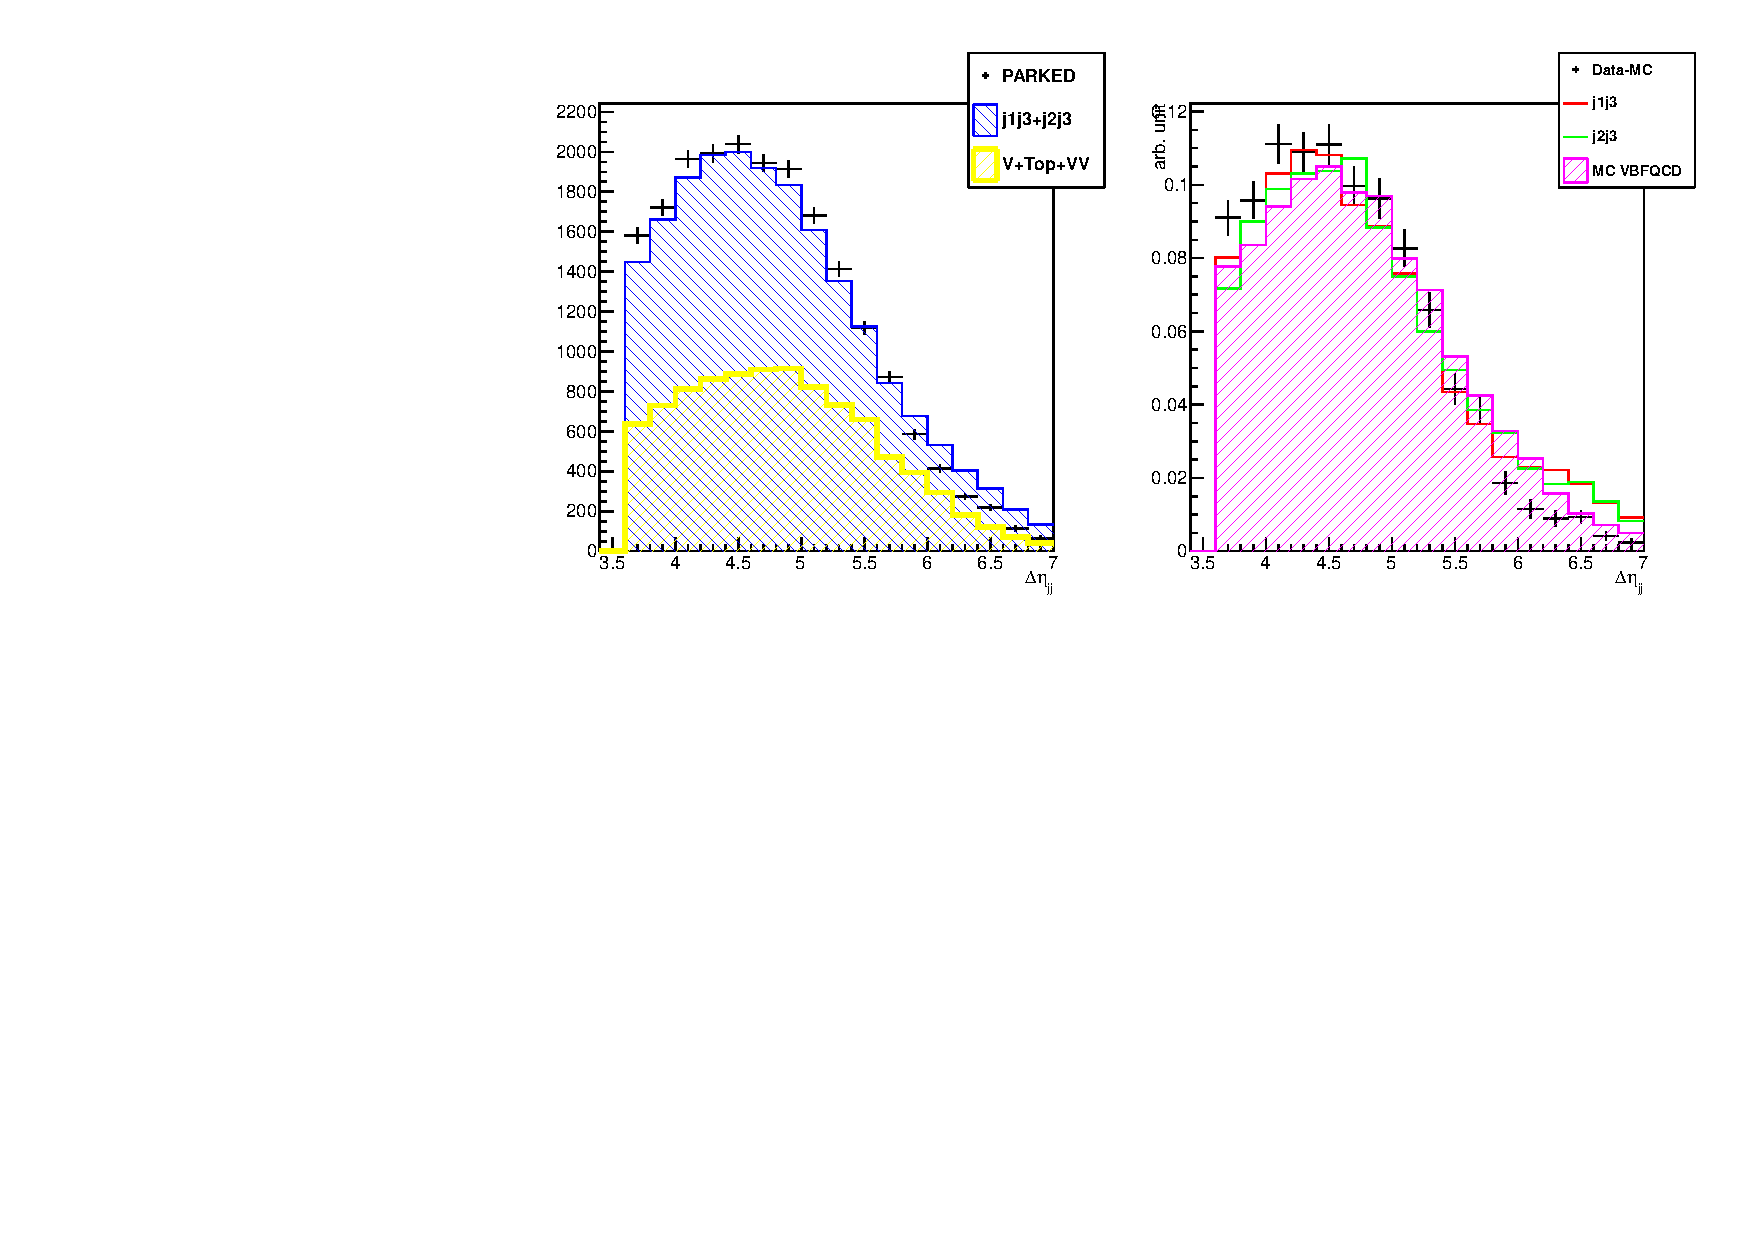
\includegraphics[width=.42\textwidth]{TalkPics/higgsexo031114/output_qcdJiJj/DataMC_PARKED_dijet_deta.pdf}
    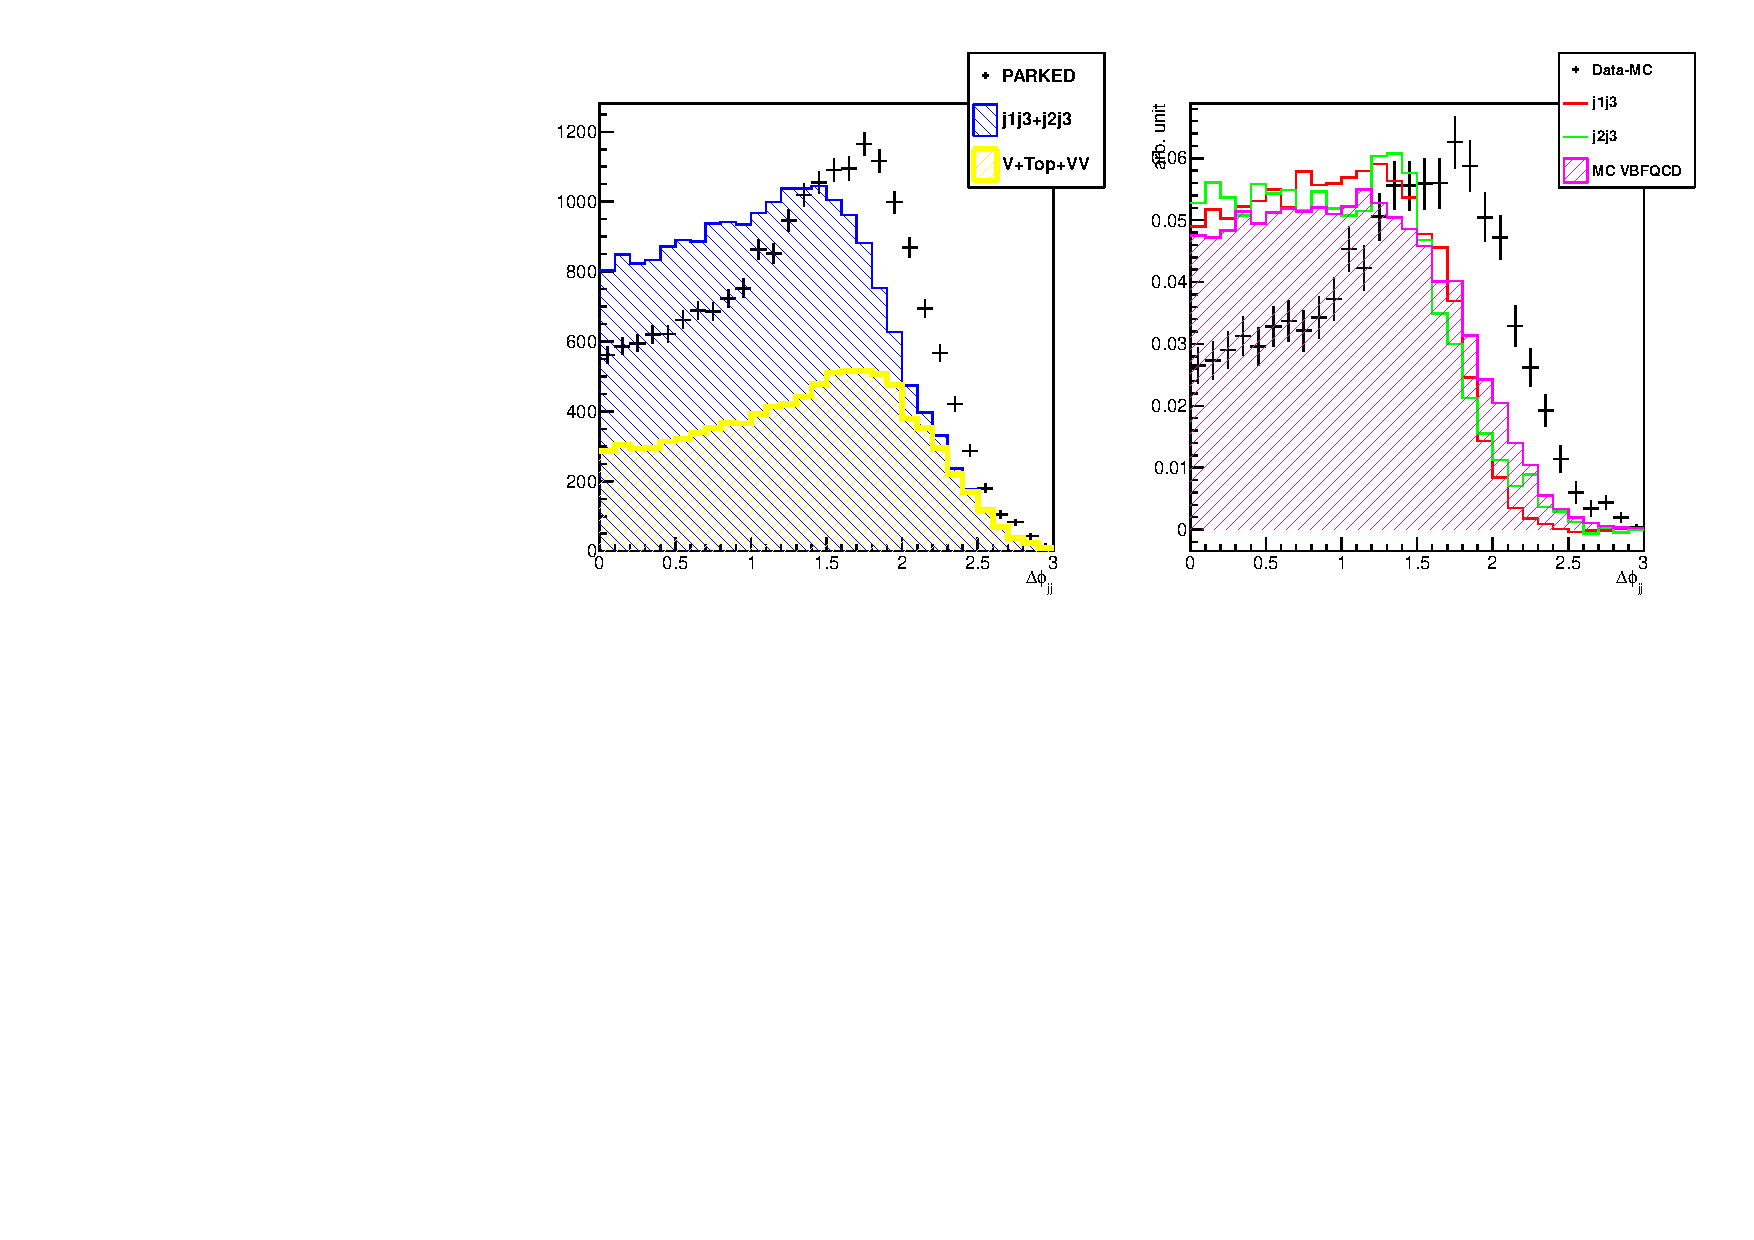
\includegraphics[width=.42\textwidth]{TalkPics/higgsexo031114/output_qcdJiJj/DataMC_PARKED_dijet_dphi.pdf}

    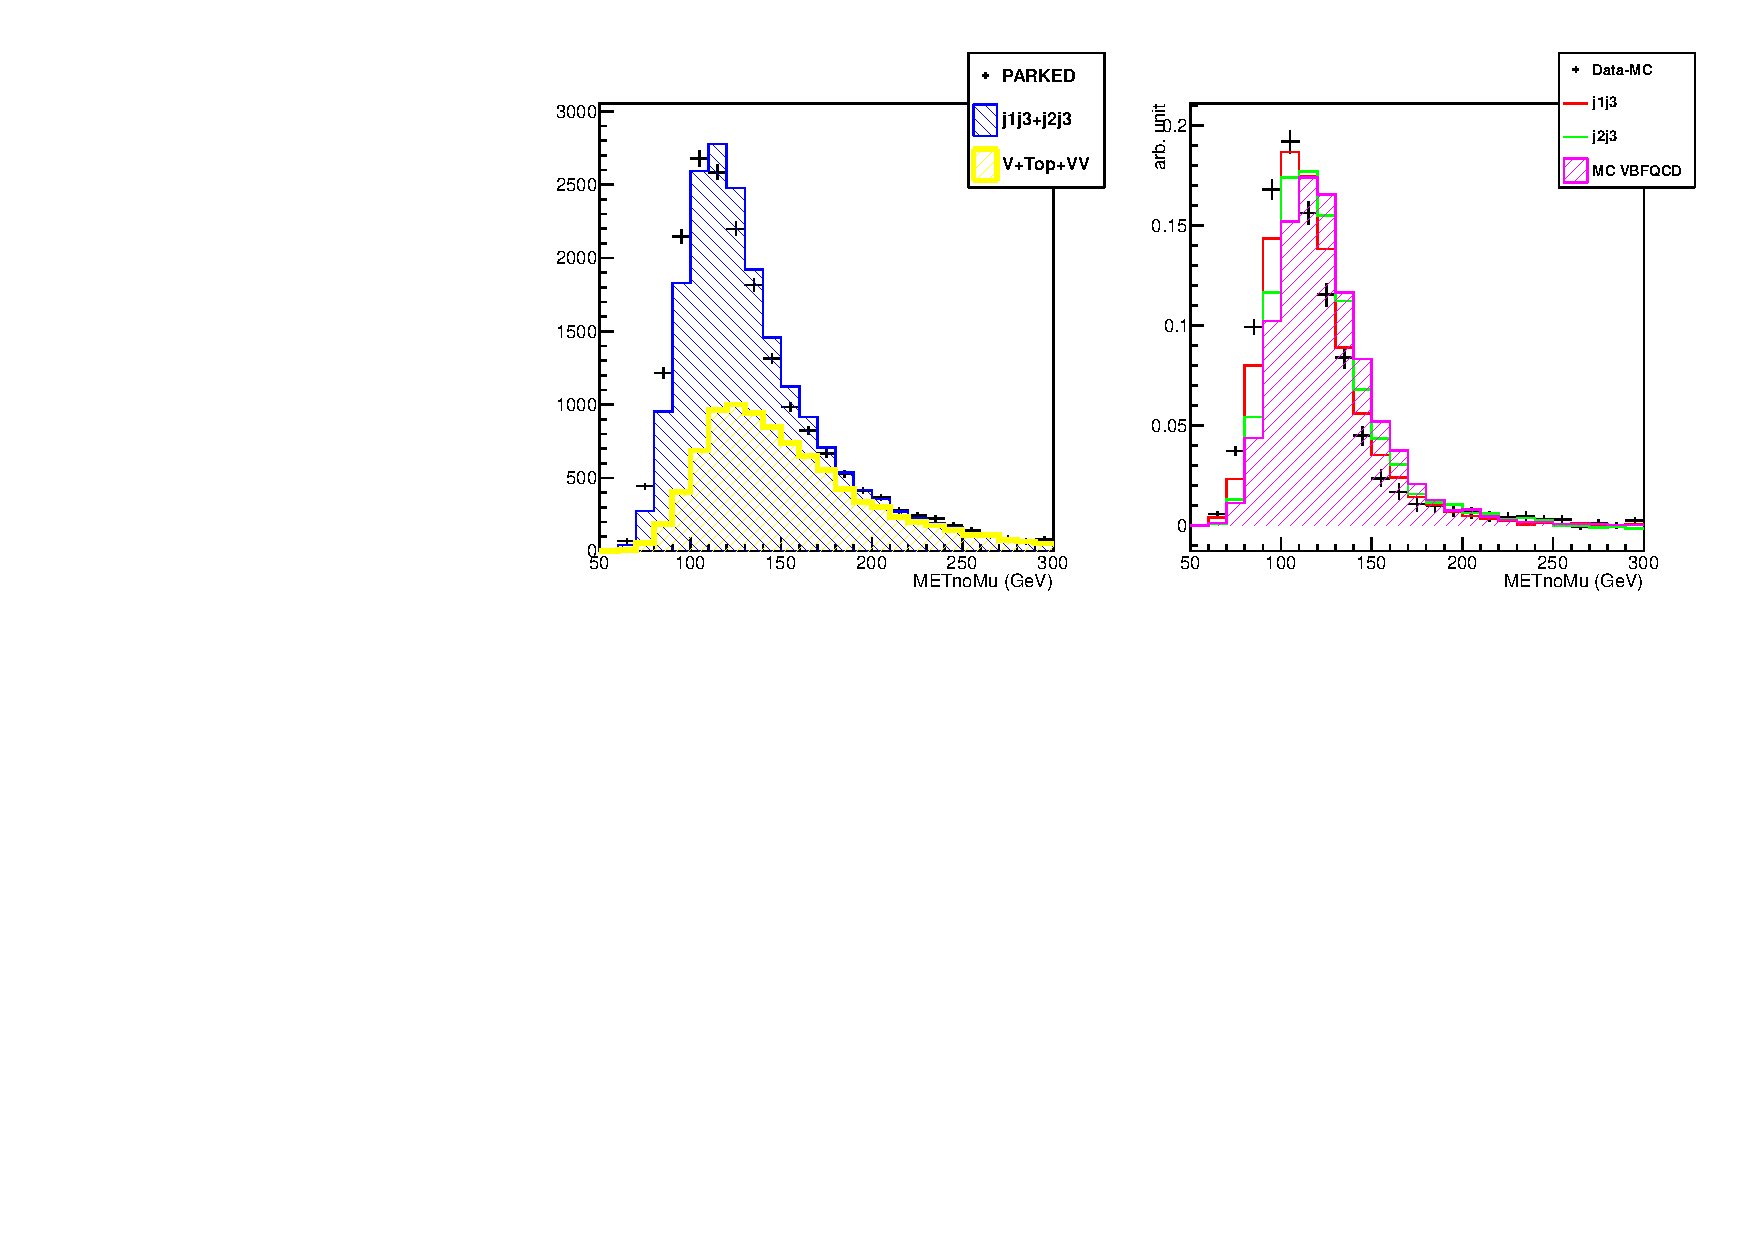
\includegraphics[width=.42\textwidth]{TalkPics/higgsexo031114/output_qcdJiJj/DataMC_PARKED_metnomuons.pdf}
    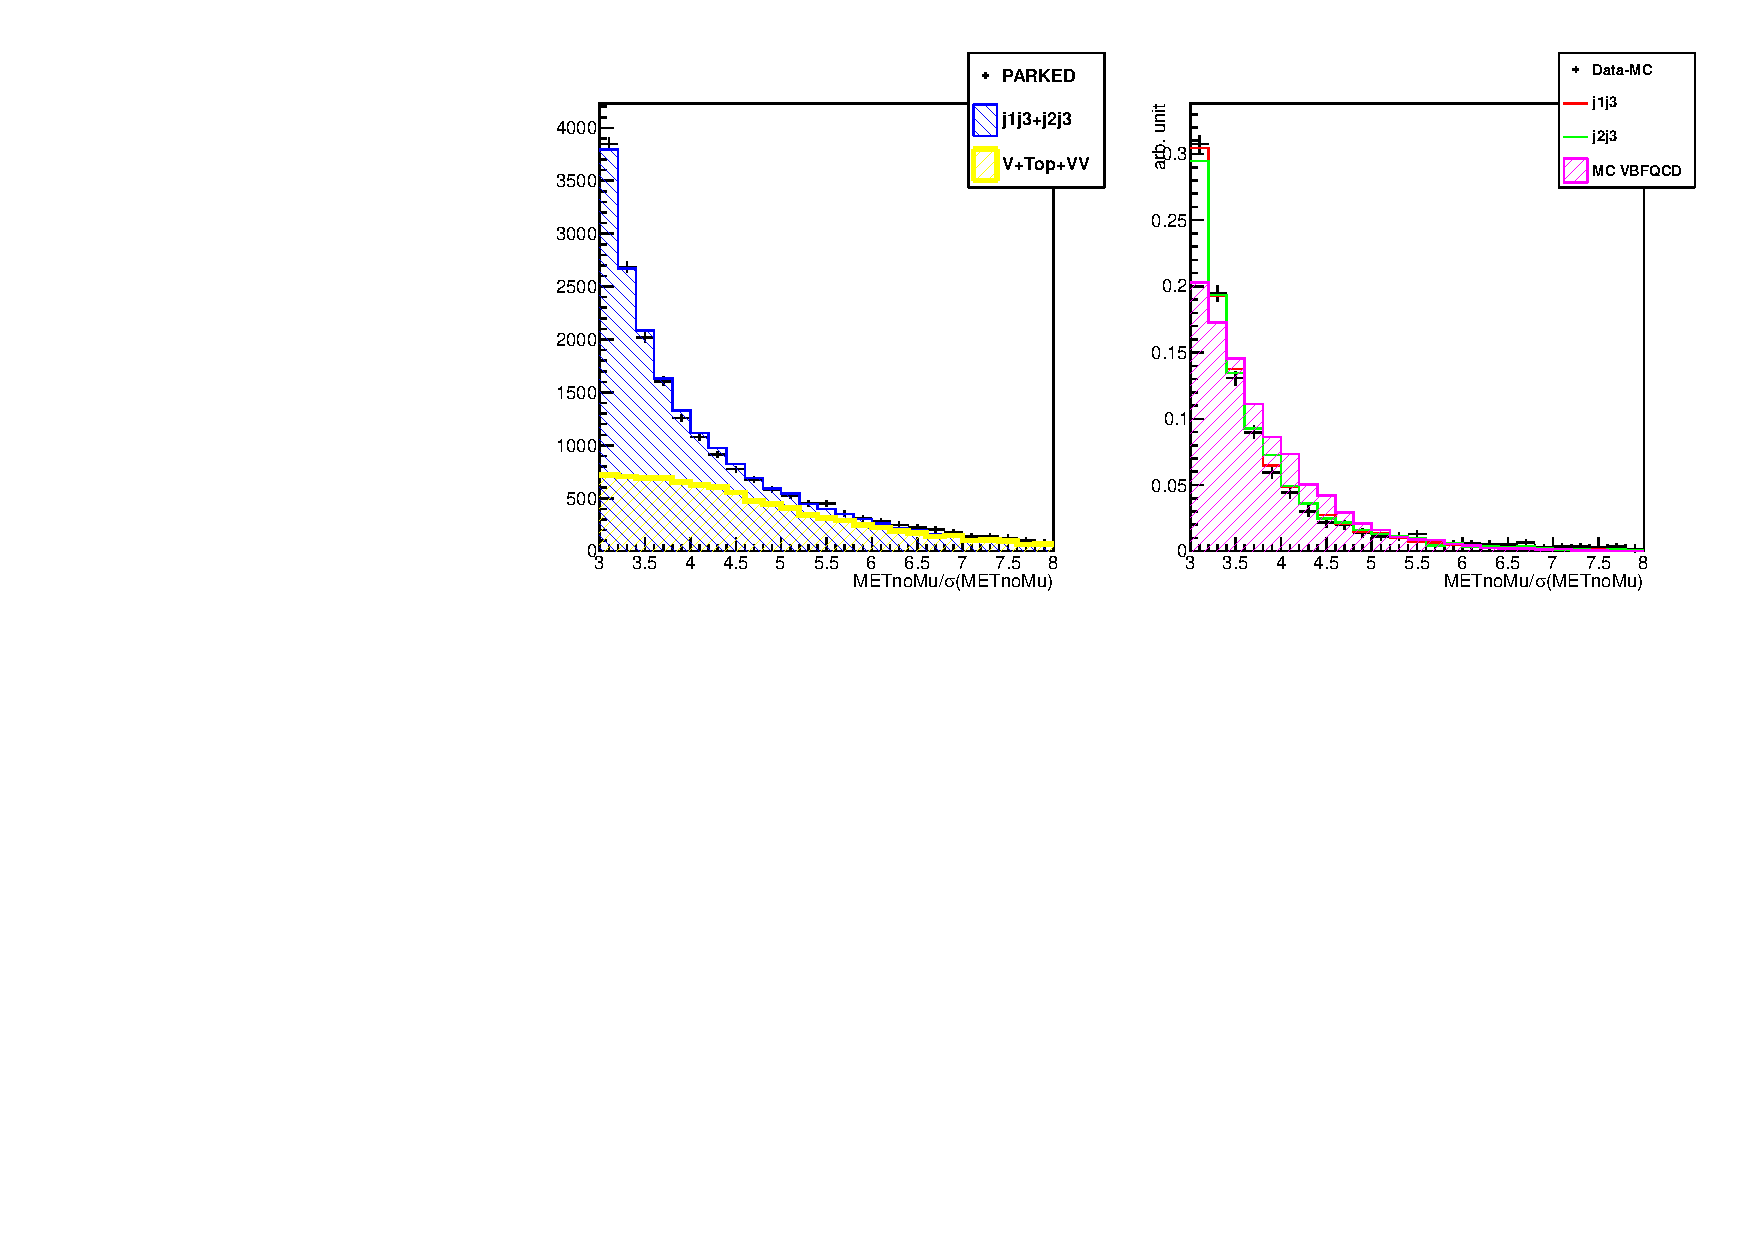
\includegraphics[width=.42\textwidth]{TalkPics/higgsexo031114/output_qcdJiJj/DataMC_PARKED_metnomu_significance.pdf}

    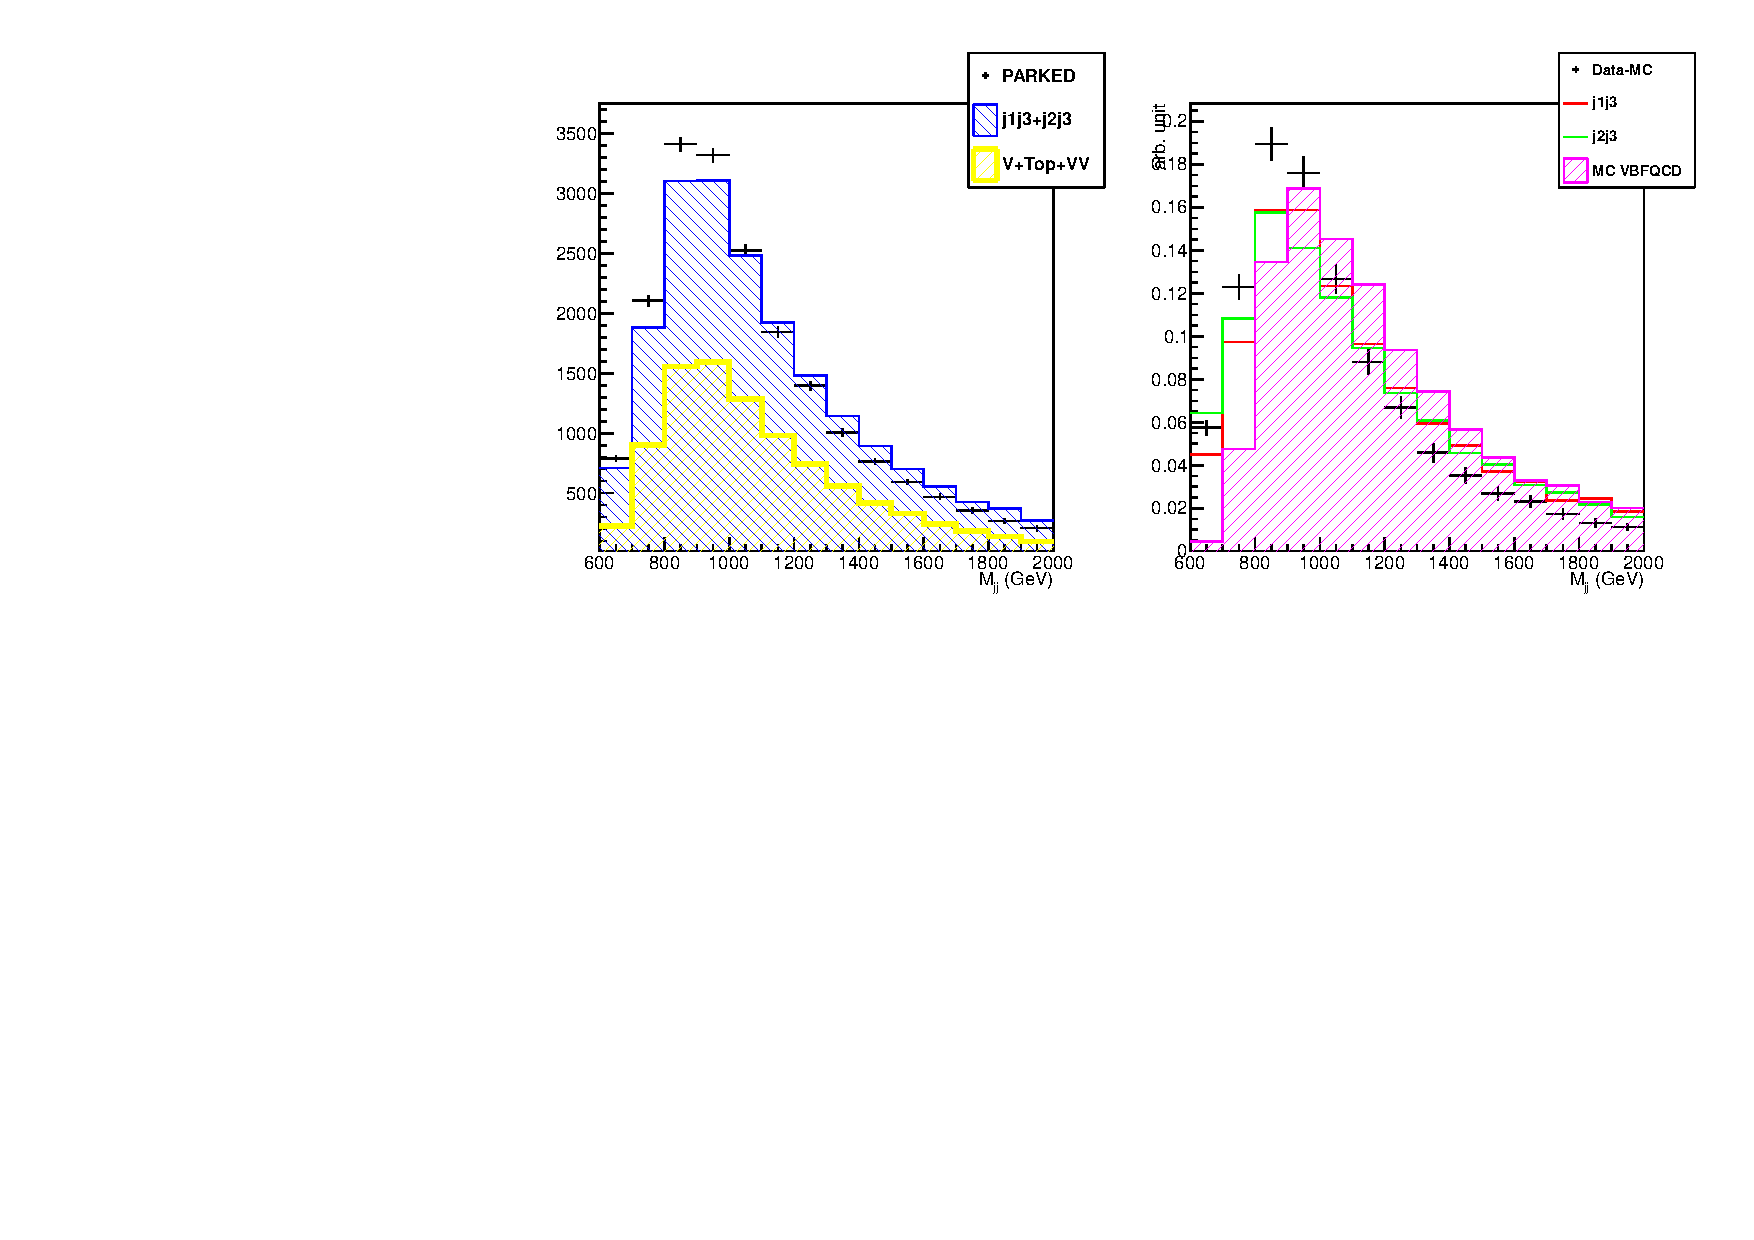
\includegraphics[width=.42\textwidth]{TalkPics/higgsexo031114/output_qcdJiJj/DataMC_PARKED_dijet_M.pdf}
    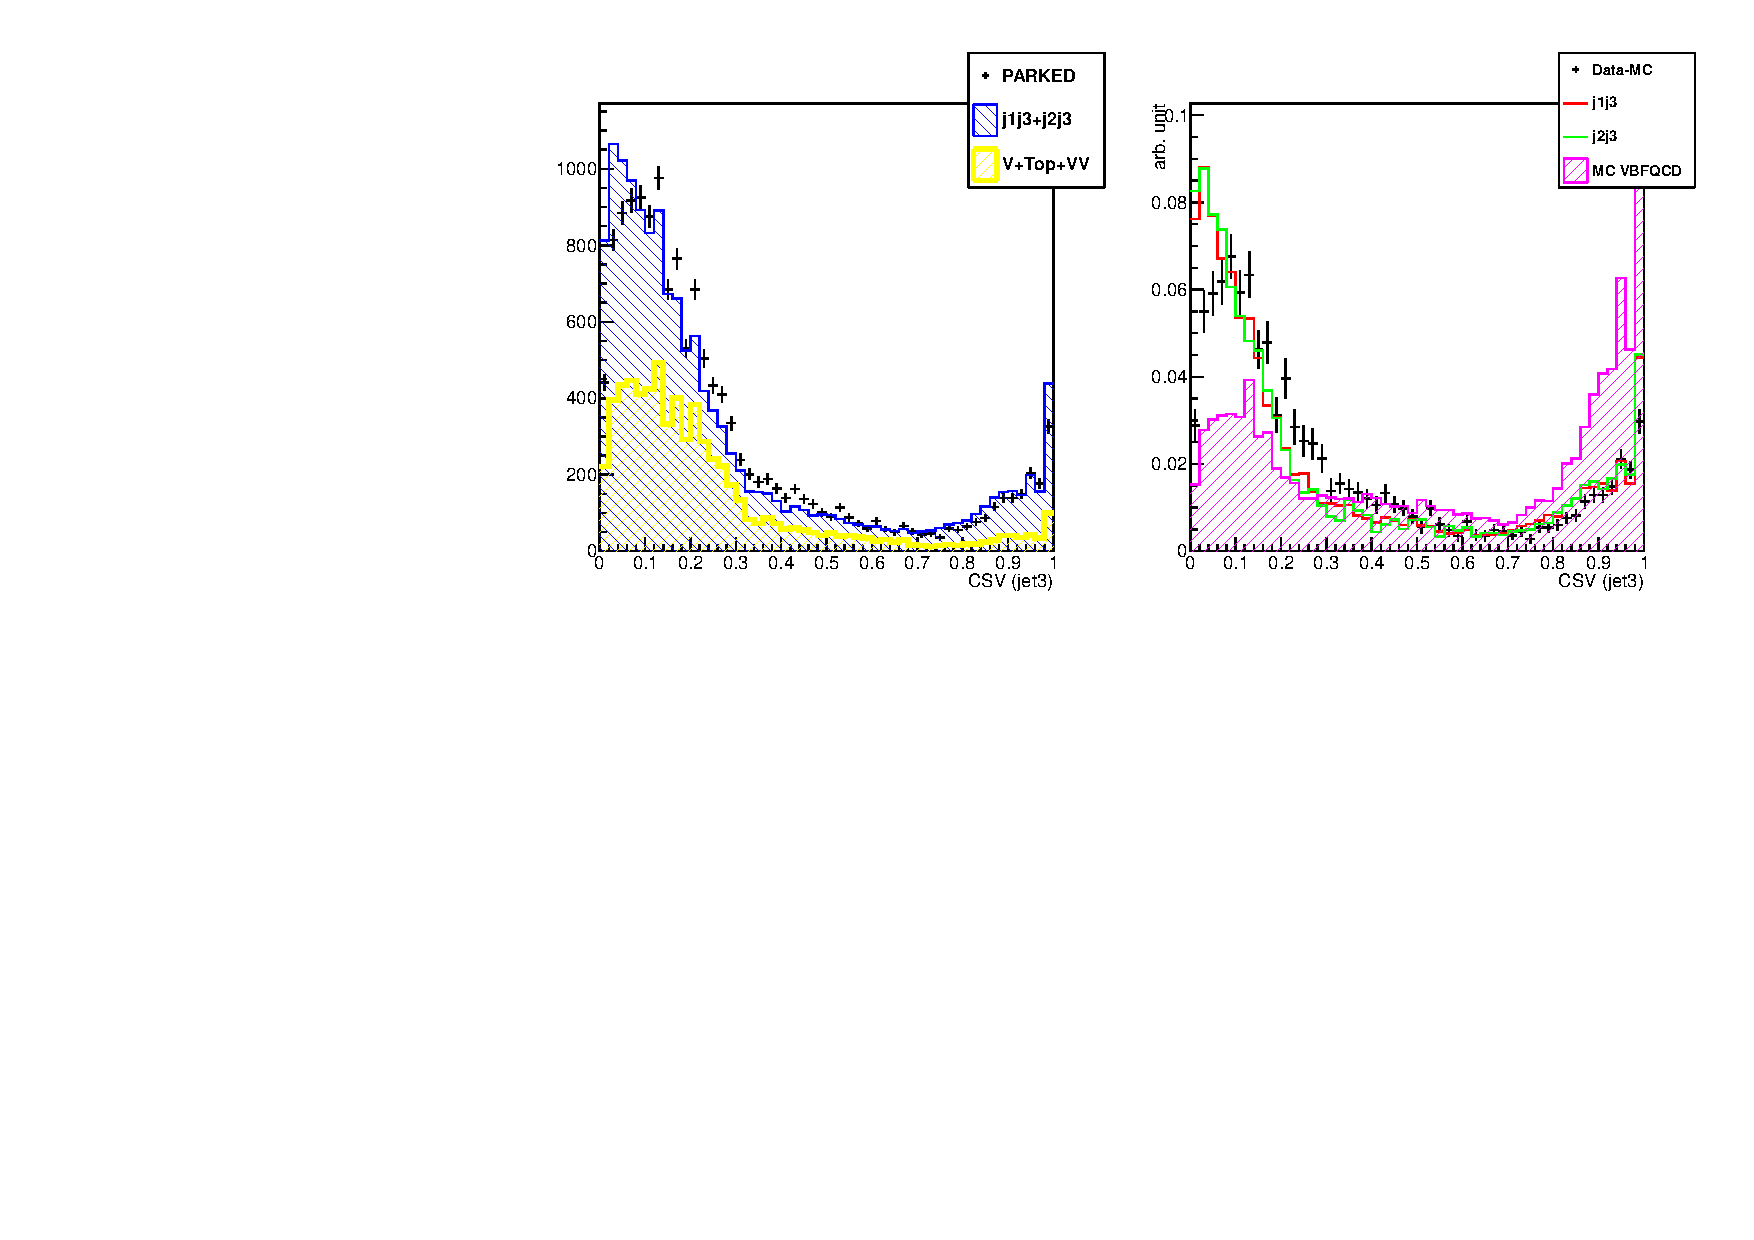
\includegraphics[width=.42\textwidth]{TalkPics/higgsexo031114/output_qcdJiJj/DataMC_PARKED_jet3_csv.pdf}

\end{frame}

\begin{frame}
  \frametitle{MVA Details}
  \centering
  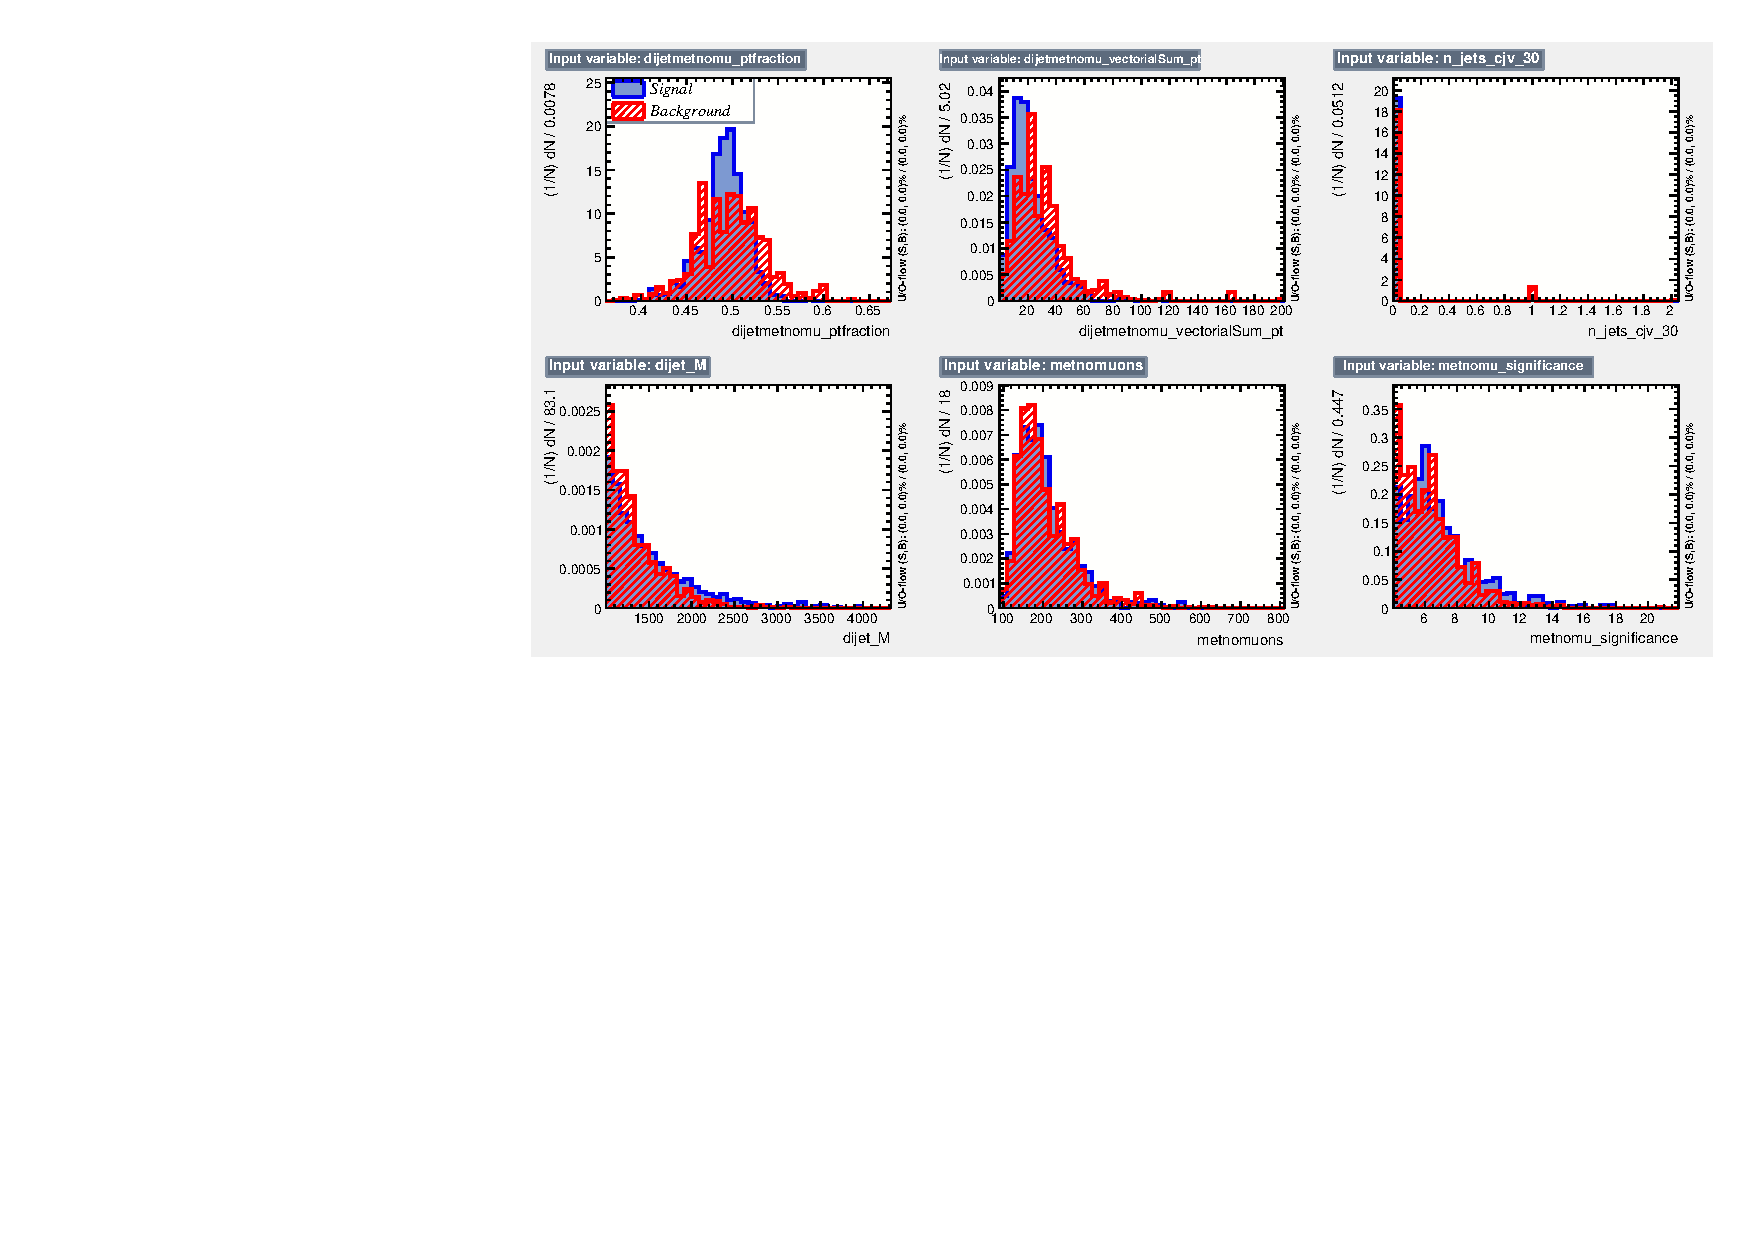
\includegraphics[width=.75\textwidth]{TalkPics/higgsexo031114/mvainputs1.pdf}

  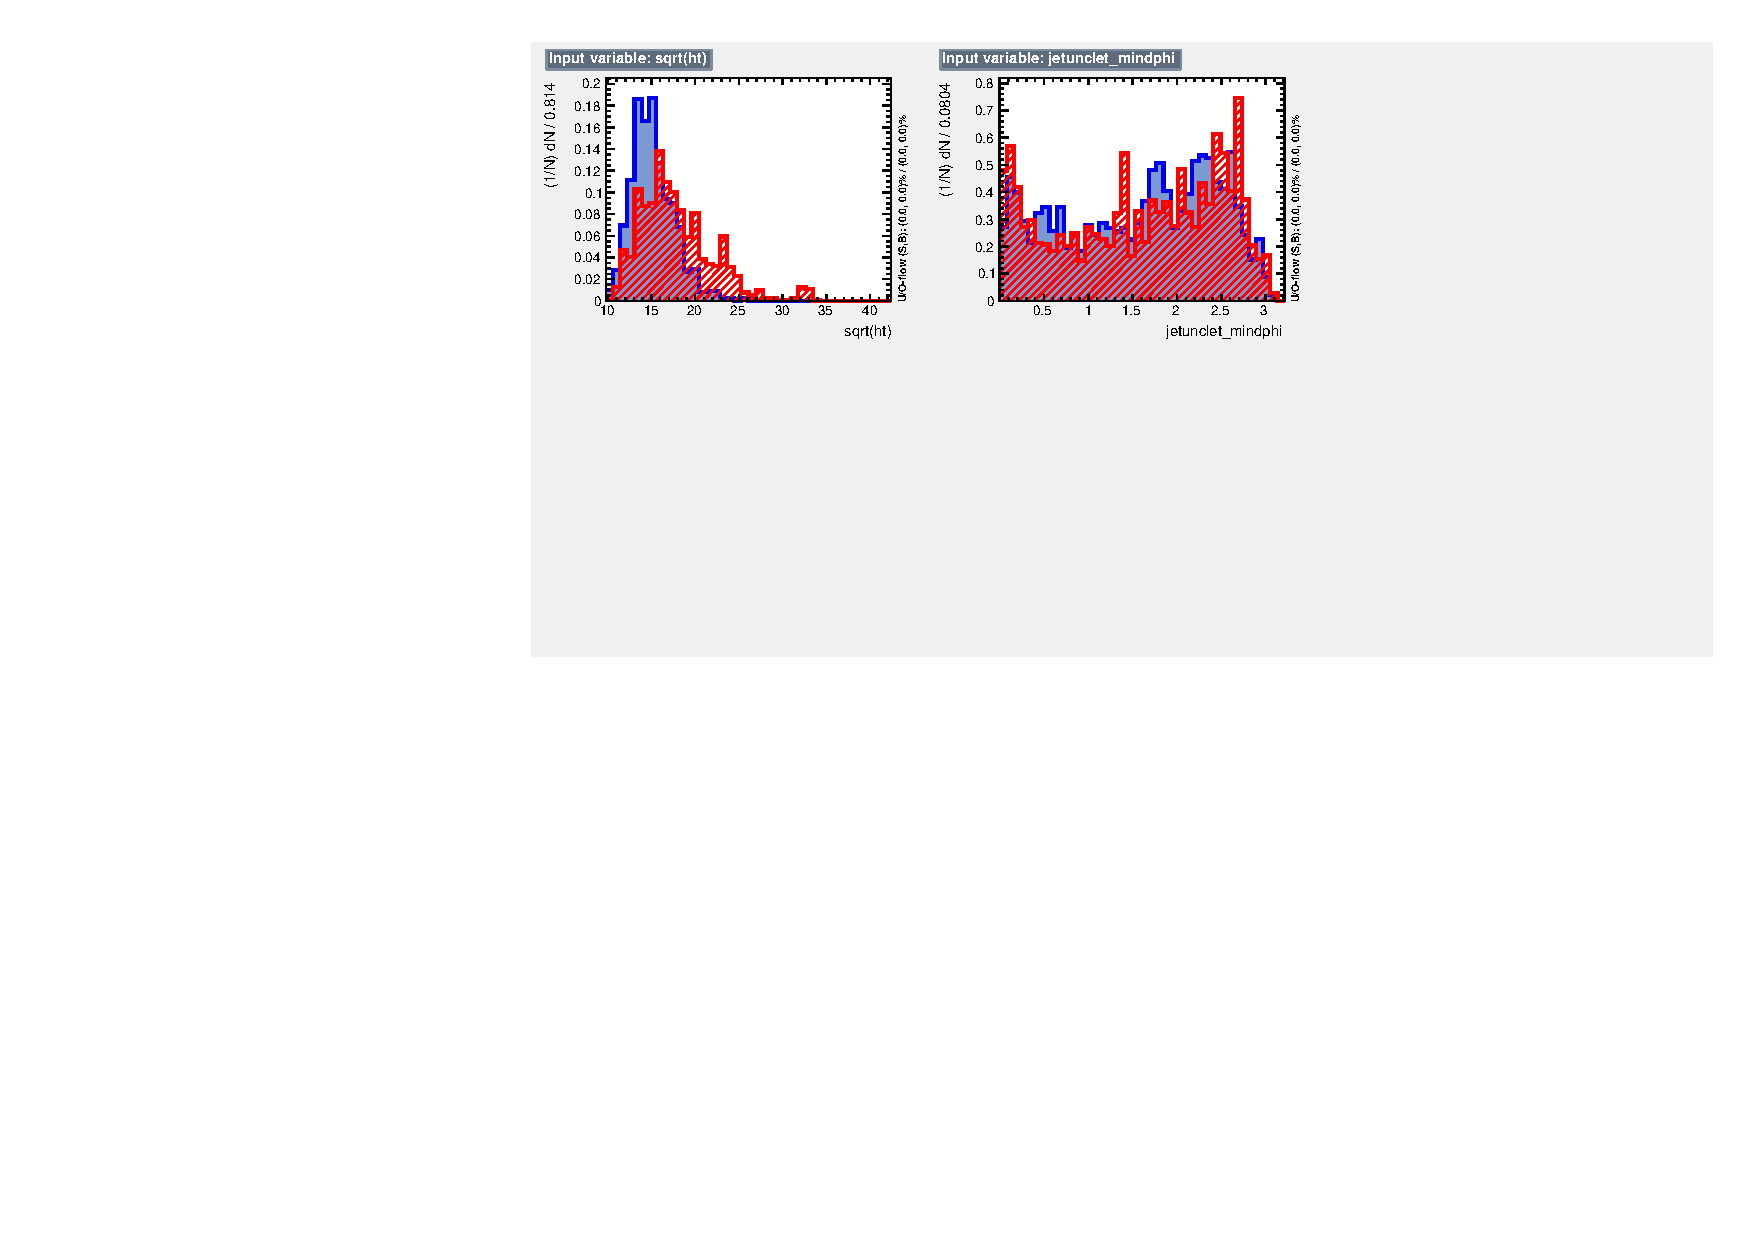
\includegraphics[clip=true,trim=0 140 0 0 ,width=.75\textwidth]{TalkPics/higgsexo031114/mvainputs2.pdf} 
\end{frame}

\begin{frame}
  \frametitle{MVA Details}
  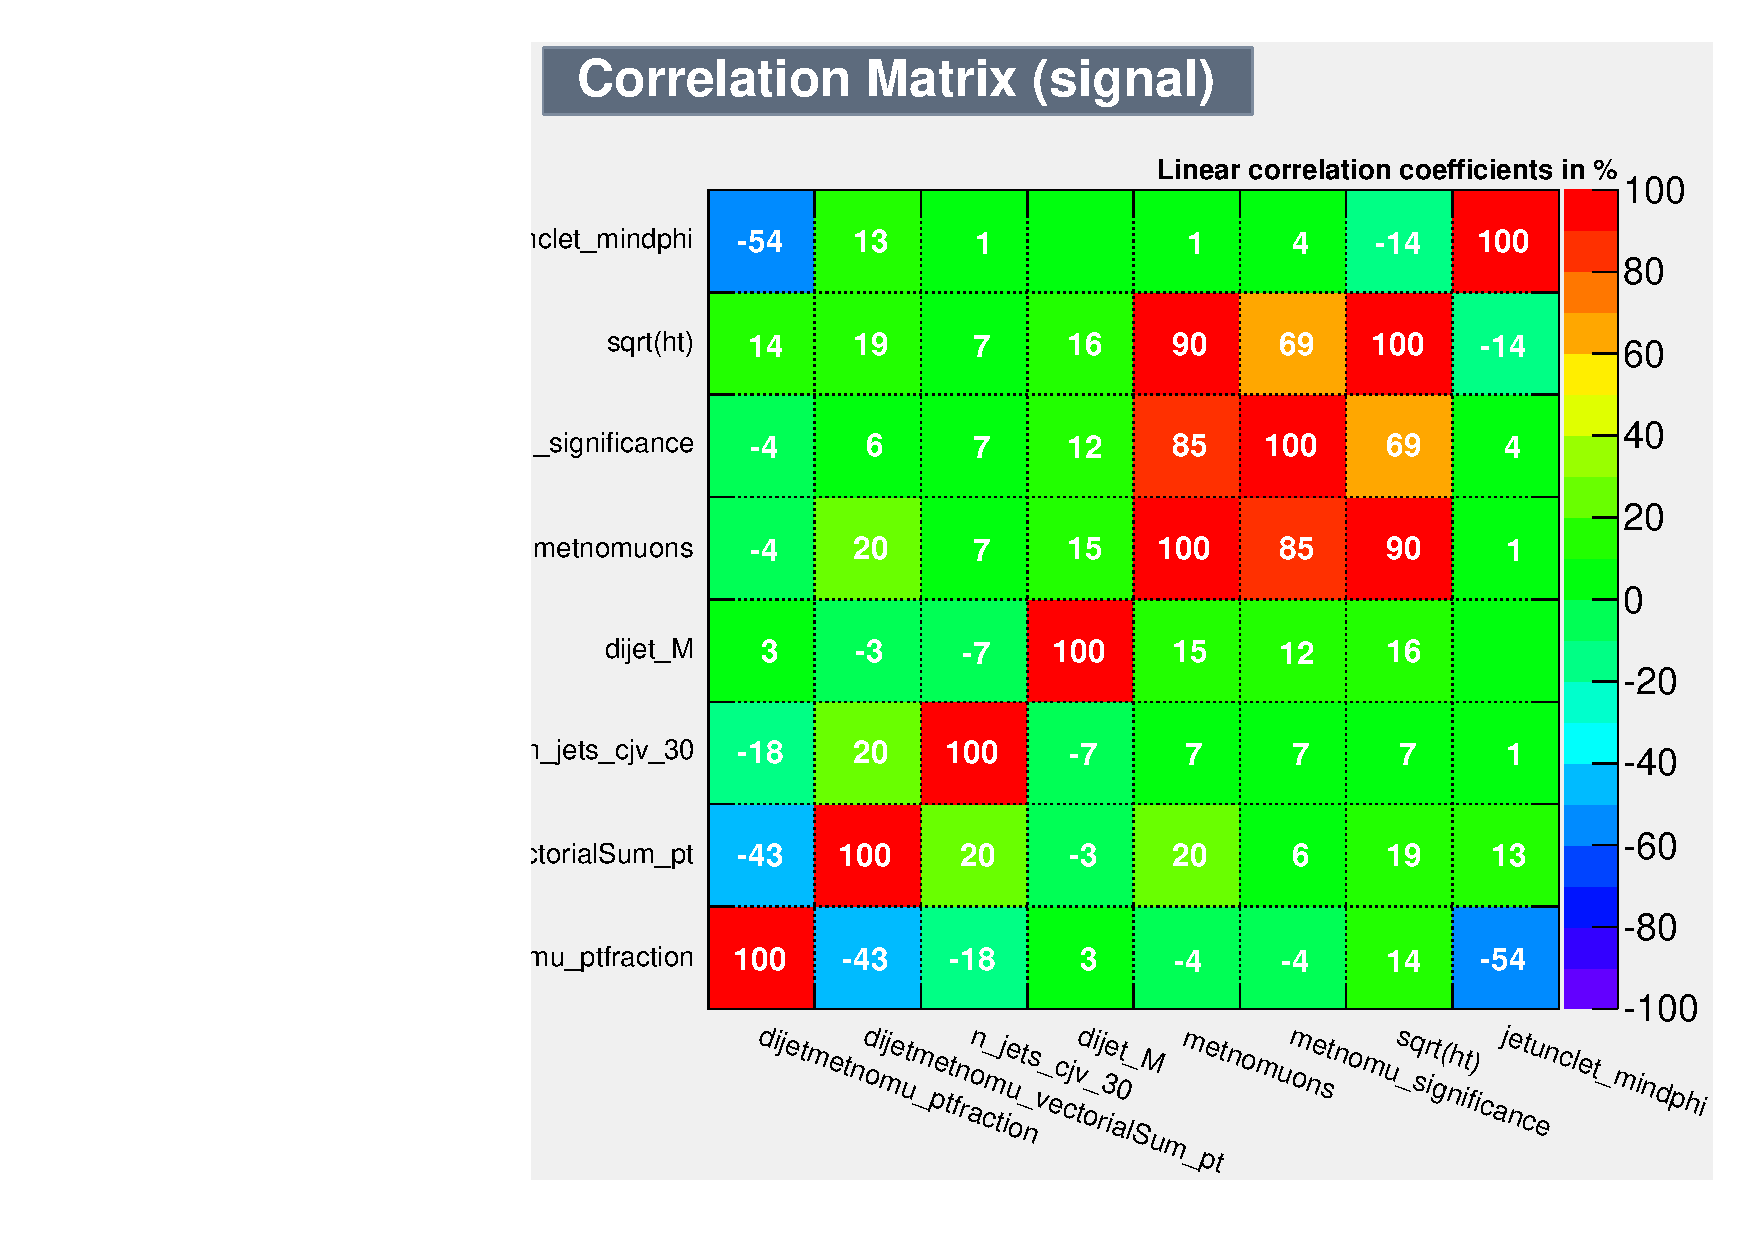
\includegraphics[width=.49\textwidth]{TalkPics/higgsexo031114/inputcorrsig.pdf}
  \hspace{.1cm}
  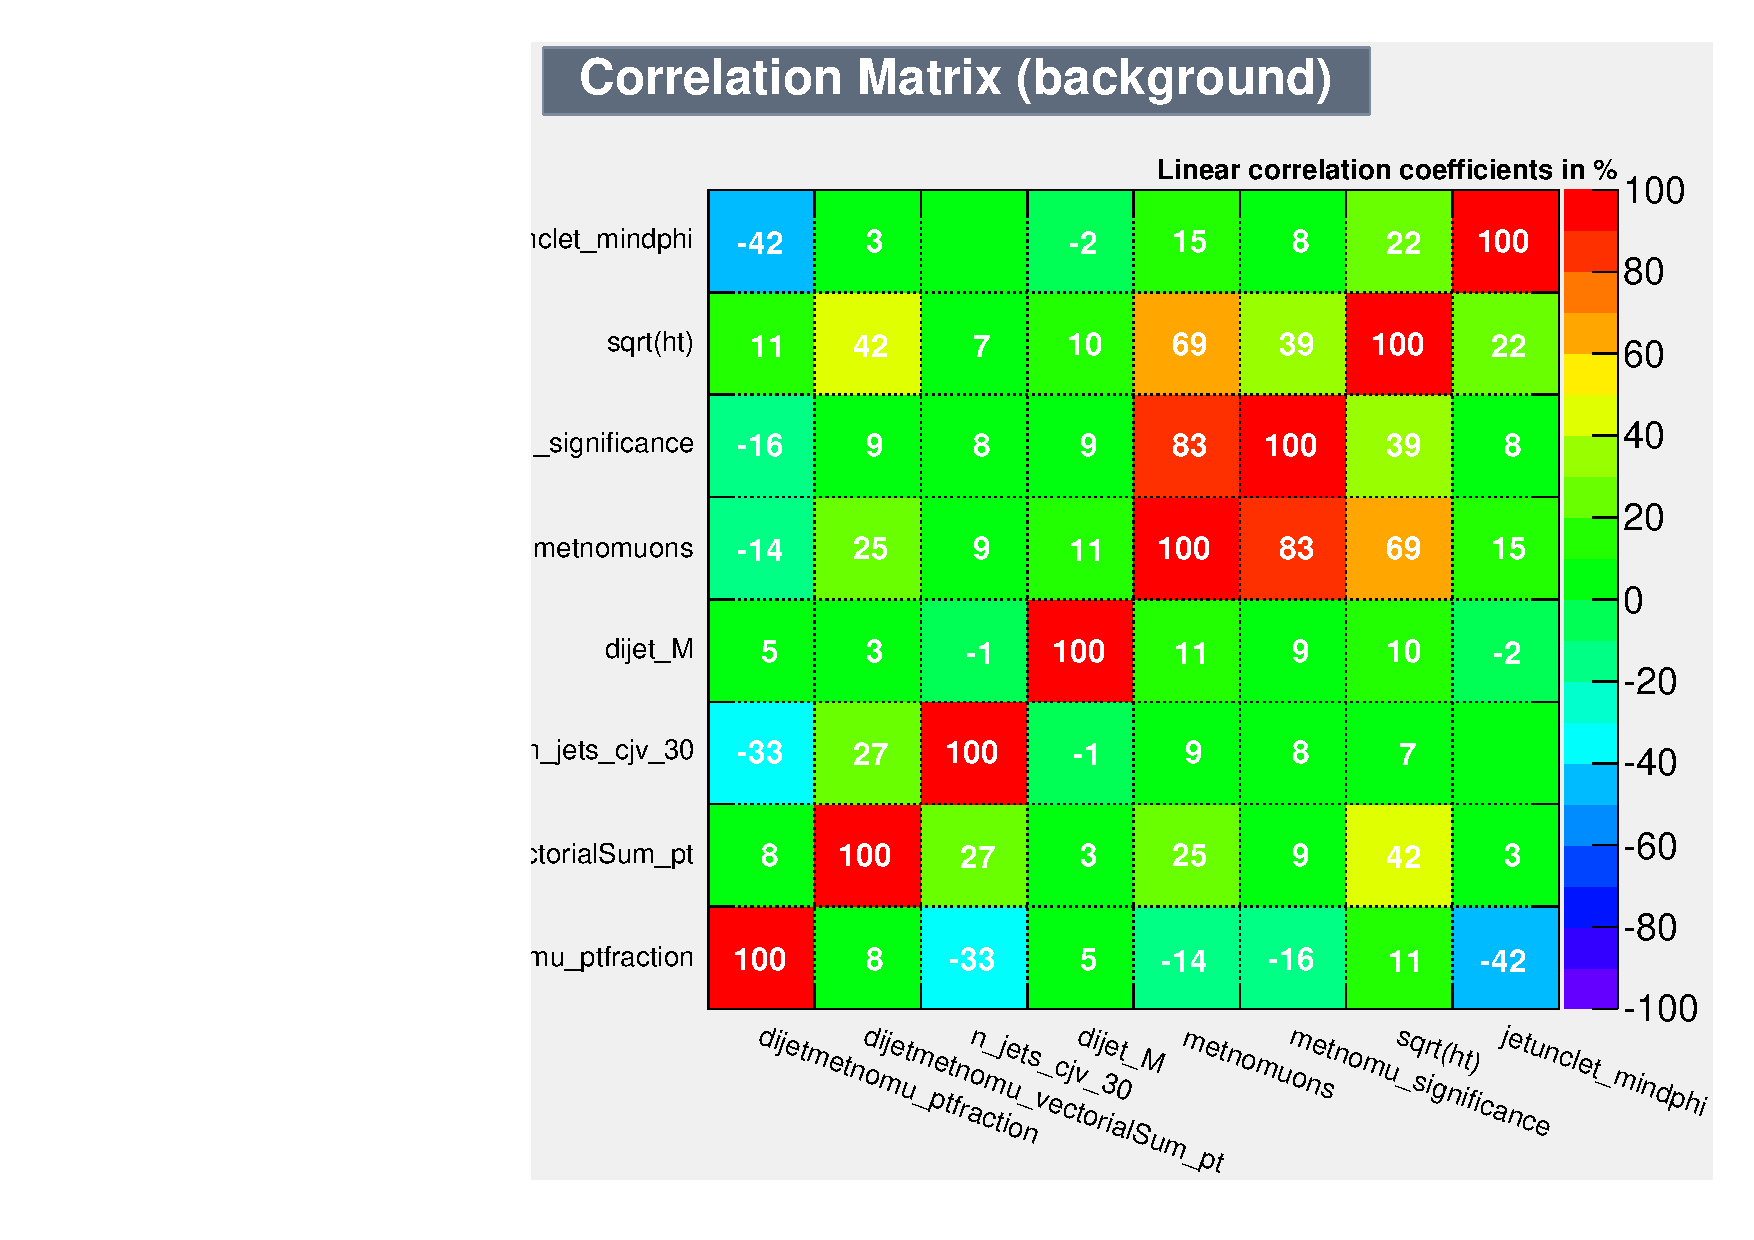
\includegraphics[width=.49\textwidth]{TalkPics/higgsexo031114/inputcorrbkg.pdf} 
\end{frame}

\begin{frame}
  \frametitle{MVA Details}
  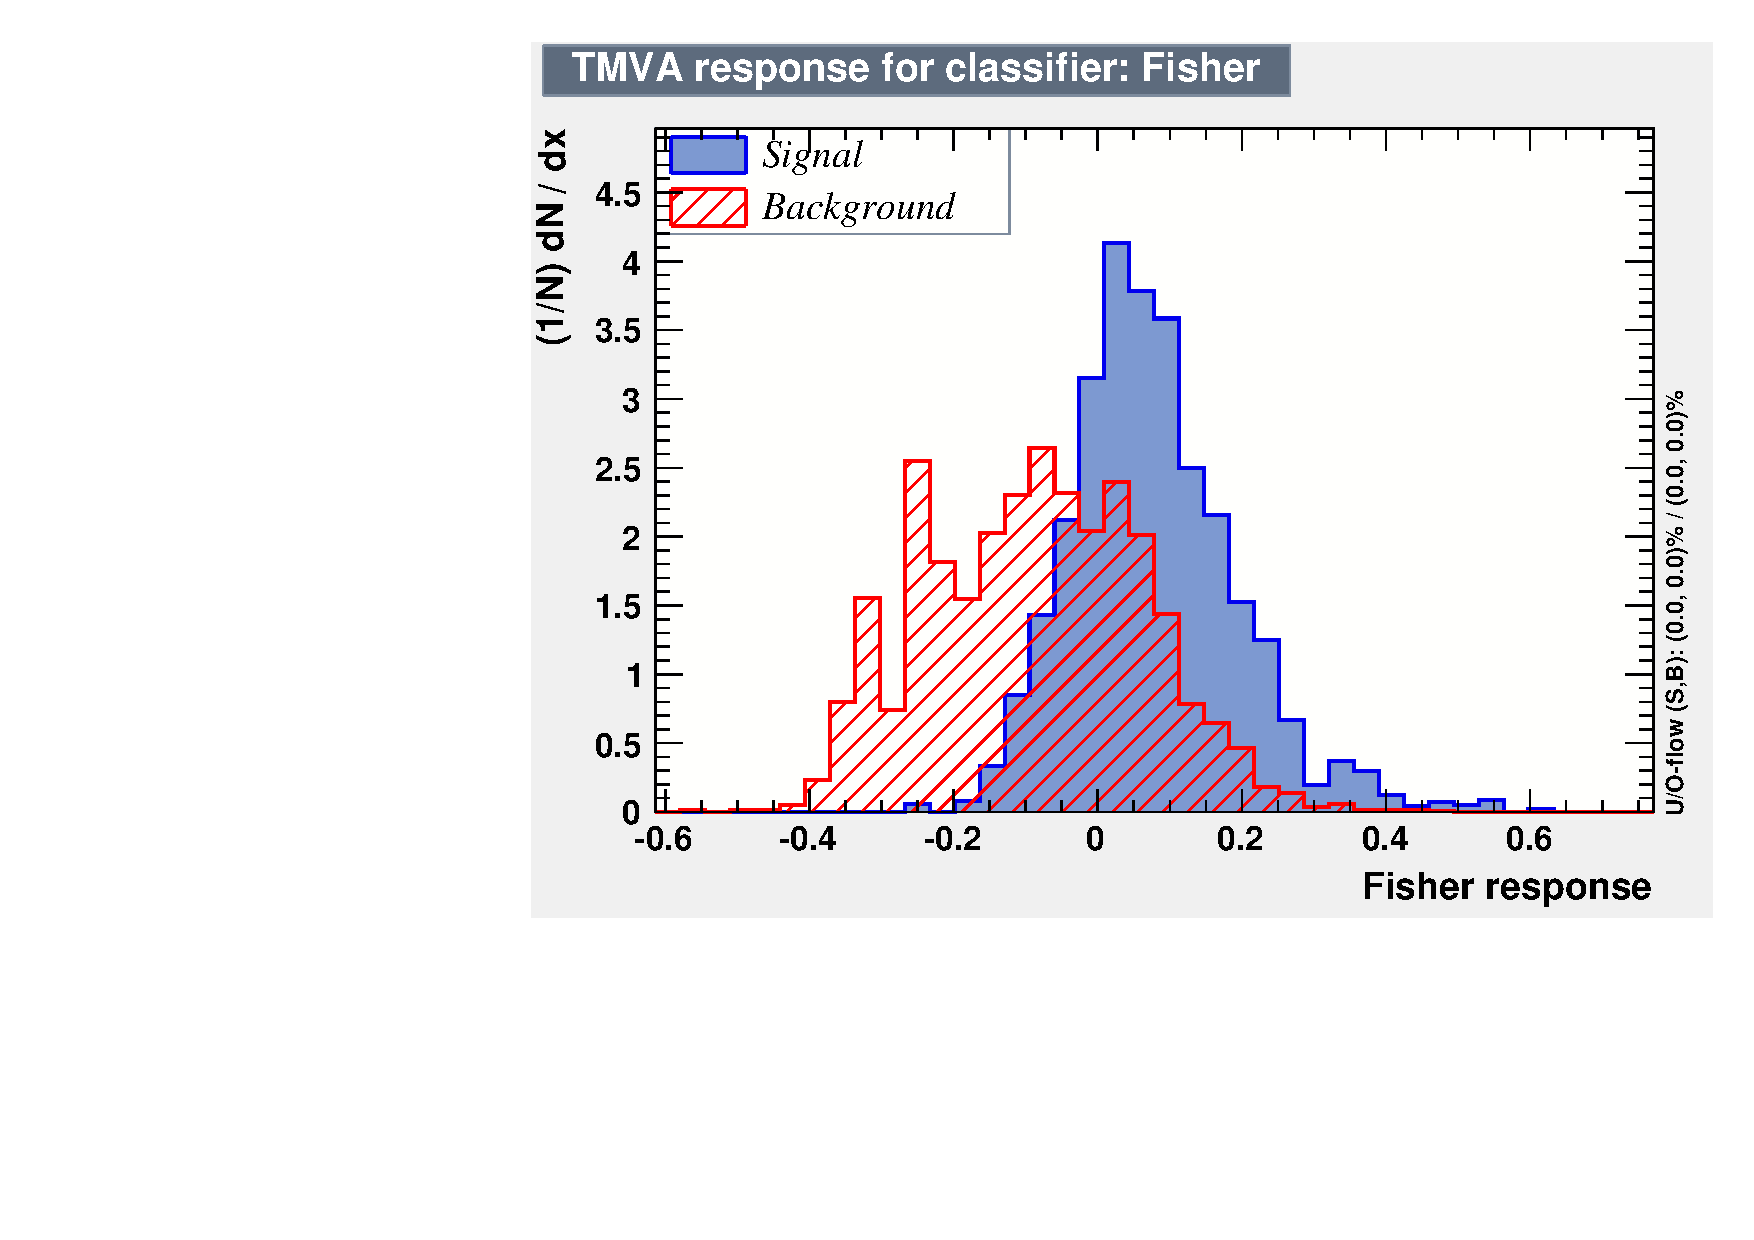
\includegraphics[width=.49\textwidth]{TalkPics/higgsexo031114/fisherdist.pdf}
  \hspace{.1cm}
  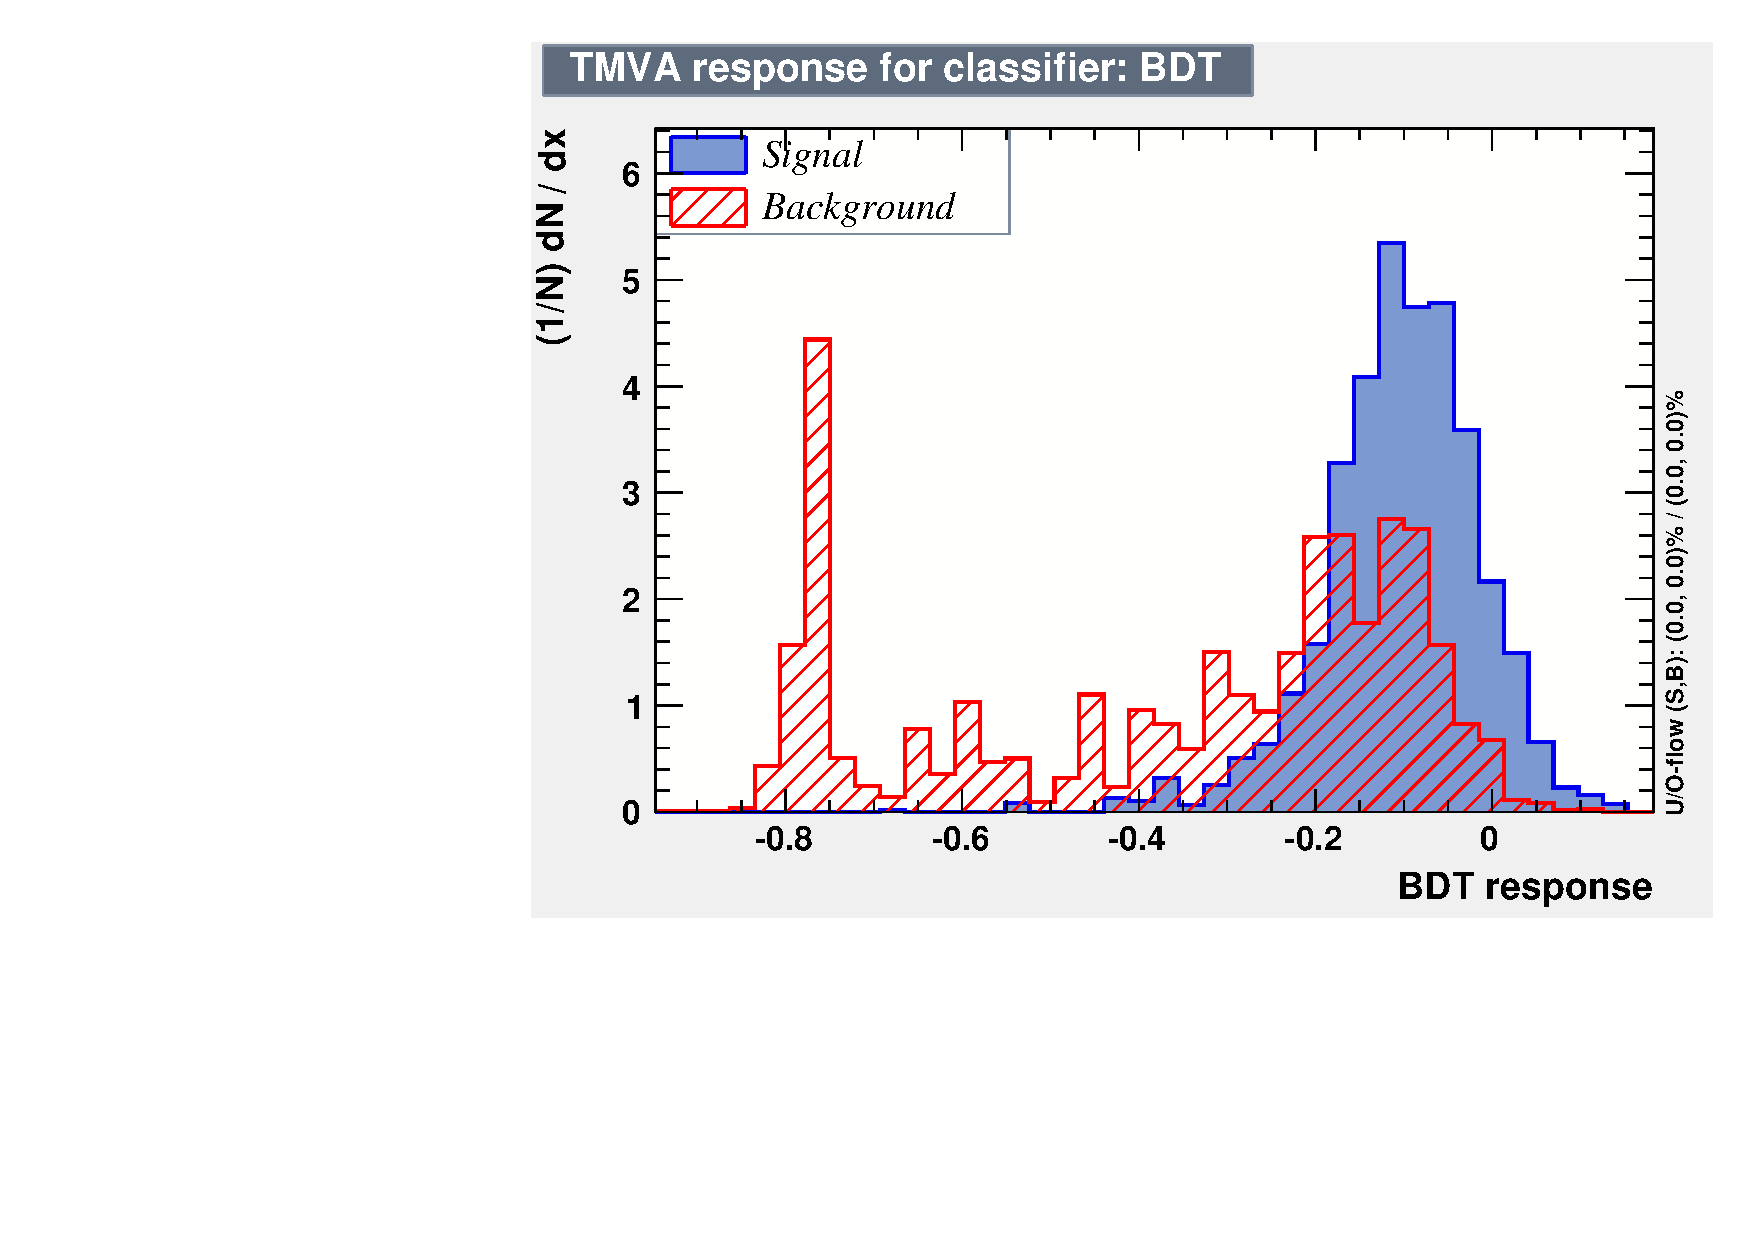
\includegraphics[width=.49\textwidth]{TalkPics/higgsexo031114/bdtdist.pdf} 
\end{frame}

\begin{frame}
  \frametitle{MVA Details}
  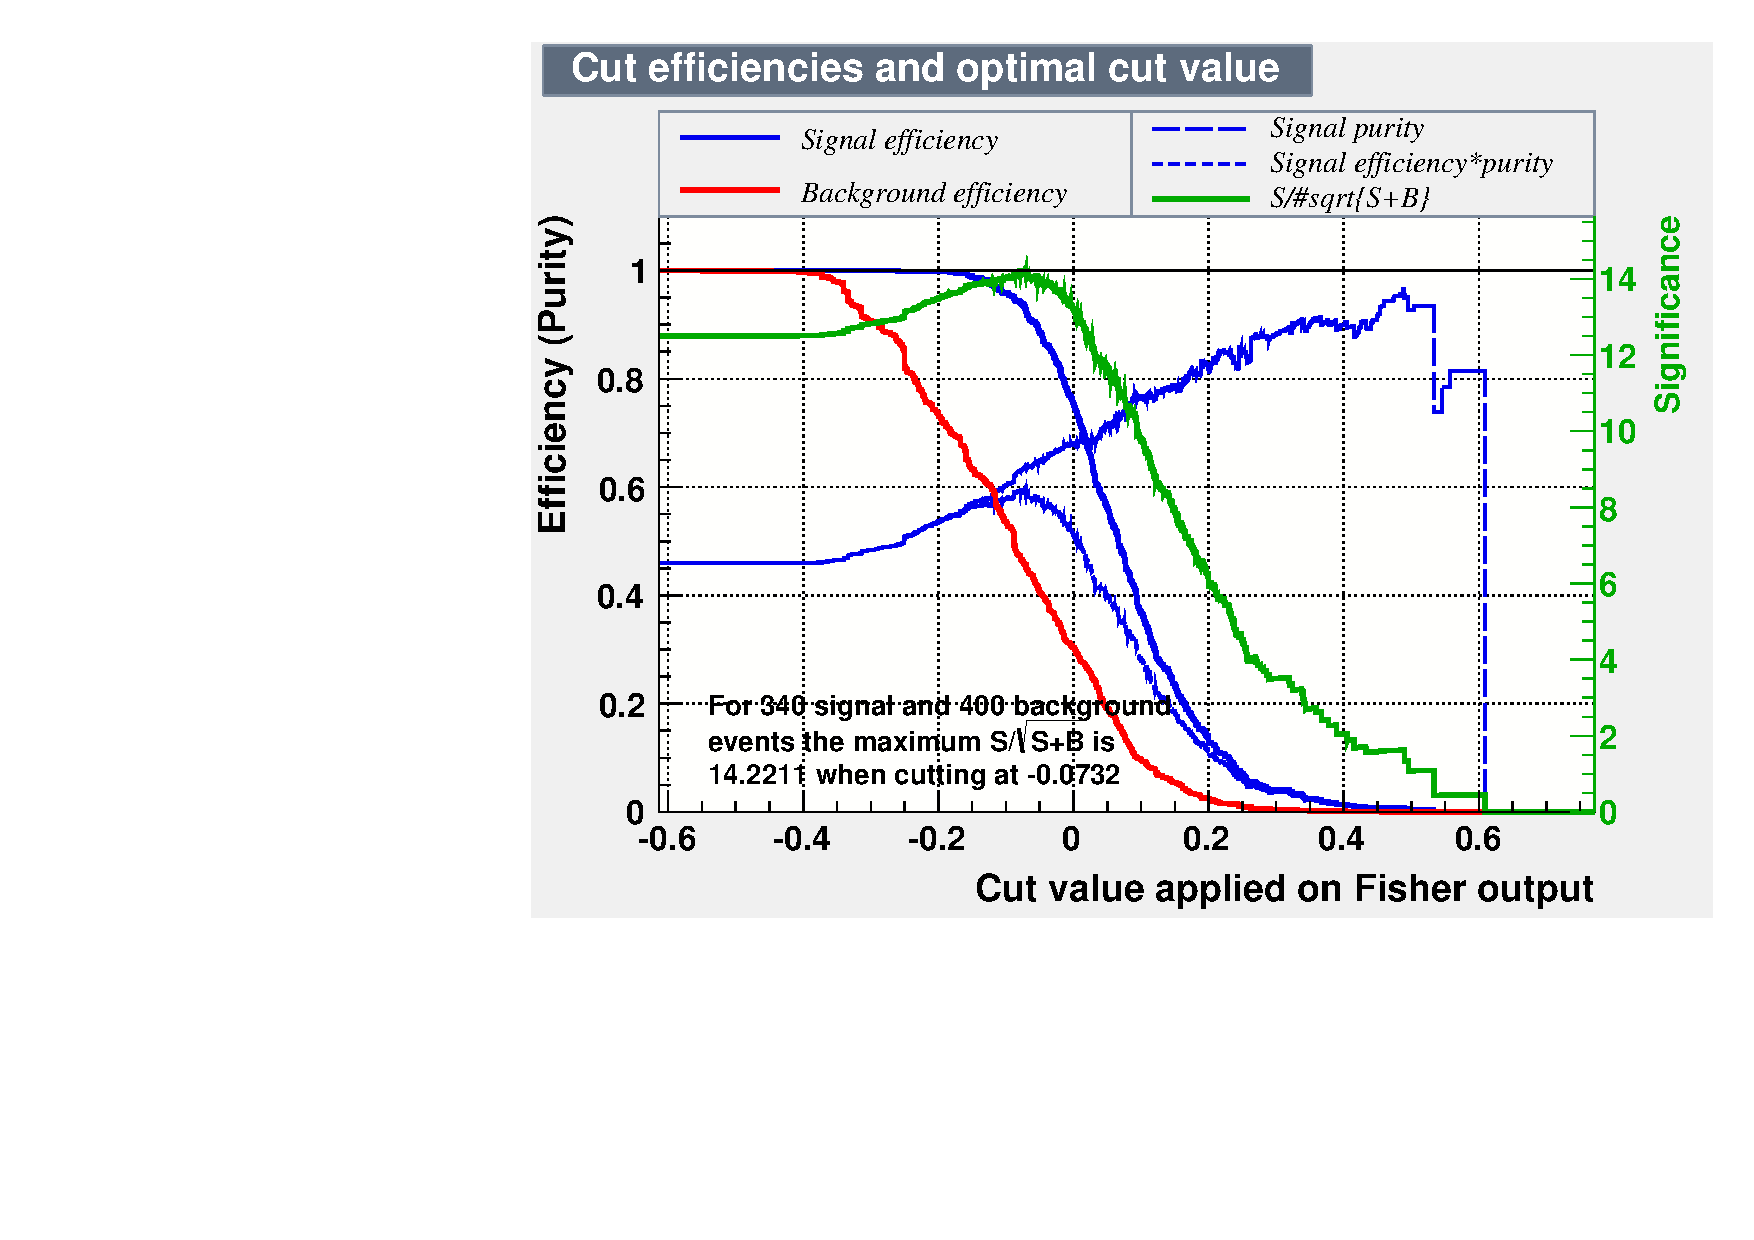
\includegraphics[width=.49\textwidth]{TalkPics/higgsexo031114/fishersoverb.pdf}
  \hspace{.1cm}
  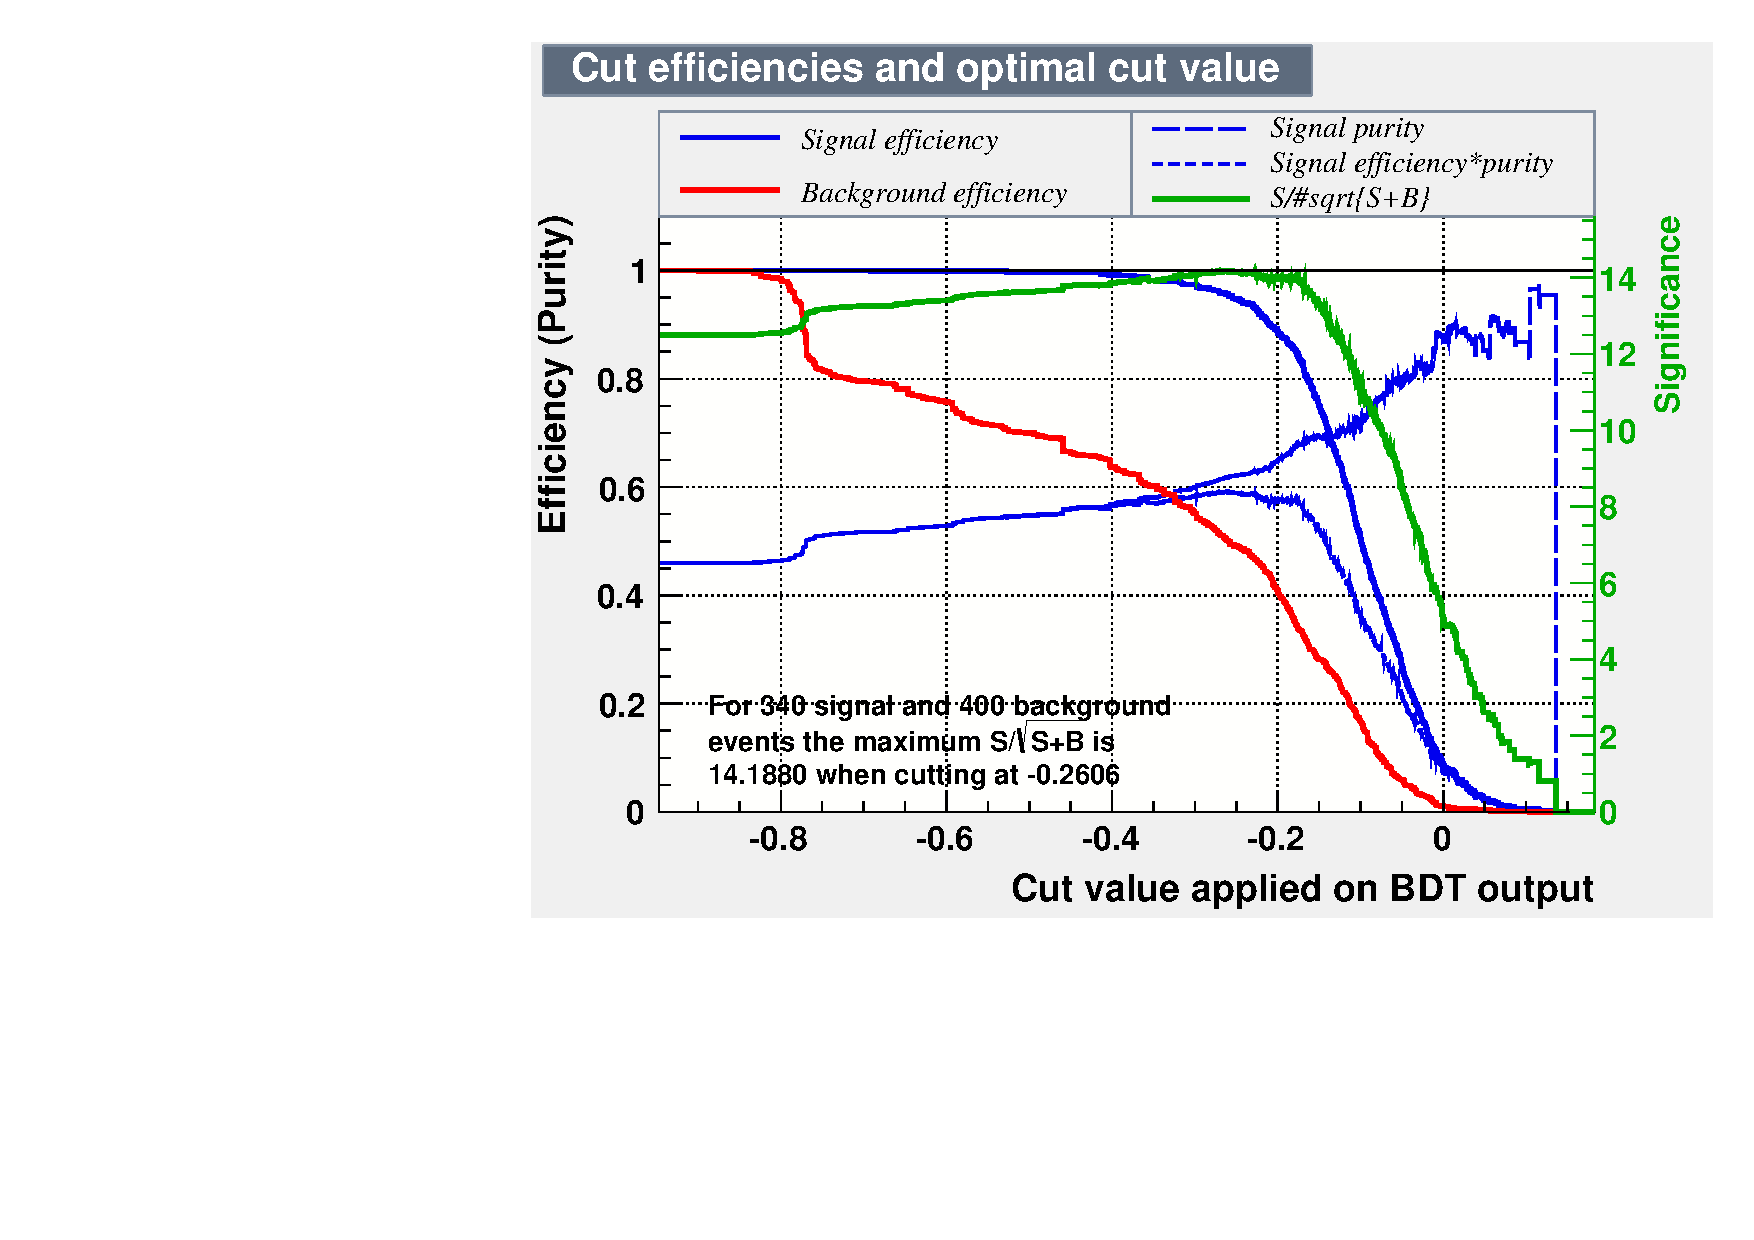
\includegraphics[width=.49\textwidth]{TalkPics/higgsexo031114/bdtsoverb.pdf} 
\end{frame}






\end{fmffile}
\end{document}
